\lhead{\begin{tikzpicture}[remember picture, overlay]
    \node [anchor=100,inner sep=0] (imagenIZQUIERDA) at (current page header area.north){
\includegraphics[width=18cm]{img/Encabezado.PNG}};
    \end{tikzpicture}}
    \rhead{Ángeles-Hurtado}
    \rfoot{\begin{tikzpicture}[remember picture, overlay]
    \node [anchor=140,inner sep=0] (imagenDERECHA) at (current page footer area.south){
\includegraphics[width=18cm]{img/Foot.PNG}};
    \end{tikzpicture}}
    %----------------------------------------------------------------------------------------
    \lfoot{ \thepage}
    % \renewcommand{\labelenumi}{\alph{enumi}.)} 
    %----------------------------------------------------------------------------------------
    %----------------------------------------------------------------------------------------
    %	TITLE SECTION
    %----------------------------------------------------------------------------------------
    
    \setlength{\droptitle}{-5\baselineskip} % Move the title up
    \title{\textbf{Estudio de tiempos y movimientos en el ensamble de un circuito electrónico utilizando diferentes métodos para su optimización }} % Article title
    
     \author{ 
     \textsc{Apellidos, Nombre/s}\\ 
    %  Afiliación:
     \texttt{ Nombre Instituto } \\ 
     \texttt{Nombre de la Organización } \\ 
     \texttt{Ciudad y País}\\ 
     \texttt{Correo} 
     \and 
     \textsc{Corona Cruz, Alan Gael}\\ 
    %  Afiliación:
     \texttt{ Instituto Tecnológico de Querétaro } \\ 
     \texttt{ Tecnológico Nacional de México } \\ 
     \texttt{Querétaro, México}\\ 
     \texttt{} 
    }
    
    
    %----------------------------------------------------------------------------------------
    
    % \begin{document}
    
    % Print the title
    \maketitle
    \thispagestyle{fancy}
    
    %----------------------------------------------------------------------------------------
    %	ARTICLE CONTENTS
    %----------------------------------------------------------------------------------------
    
    % \section*{Resumen}
    % \textit{Palabras clave:}
    % El resumen (ancho de página) deberá contener entre 100 y 200 palabras tipo Adobe Devangari 11 puntos.
    
    \begin{abstract}
    \noindent 
    El resumen (ancho de página) deberá contener entre 100 y 200 palabras tipo Adobe Devangari 11 puntos.
    
    \end{abstract}
    % 
    % 
    \textbf{\textit{Palabras clave}}: {First keyword should be the corresponding to the research area according with the authors guide. Maximum of 6 keywords.}
    % \keywords{First keyword should be the corresponding to the research area according with the authors guide. Maximum of 6 keywords.}
    
    \section{Introducción}
    % Define estudio de tiempos y movimientos
        El estudio de tiempos y movimientos son técnicas  de medición del trabajo que se utiliza para poder establecer y definir el ritmo al que puede trabajar cualquier persona en una tarea específica, tomando en cuenta las condiciones de esta misma tarea y el espacio en el que la llevara a cabo lo cual tiene por objeto, en el ámbito del trabajo, evitar movimientos innecesarios del trabajador que sólo sirven para que el tiempo de cada operación sea mayor. \cite{Estudiodetiempos} \cite{Estudiodemovimientos}
    % define que es ensamble
        Para hacer uso de estos tipos de estudio trabajaremos en el ensamble de un circuito electrónico lo cual funcionara a través de la unión de distintas piezas, para lograr este ensamble deberemos trabajar en desarrollar un manual el cual se entregara al operador para que pueda realizar el ensamble, con esto podremos determinar, seleccionar y ajustar los elementos necesarios para optimizar el ensamble determinando el tiempo de ciclo, tiempo estándar y desarrollando diversos temas. \cite{Ensamble} 
    % define que es circuito electronico
        Un circuito es una interconexión de componentes eléctricos (como baterías, resisto-res, inductores, condensadores, interruptores, transistores, entre otros) que transportan la corriente eléctrica a través de una trayectoria cerrada.\cite{Circuitoelectronico}
    % define optimización
        Acción y efecto de optimizar. Para realizar este trabajo nos referimos a realizar el trabajo en el menor tiempo posible haciendo uso del estudio de tiempos y movimientos con el fin de optimizar de mejor manera.
    % define el metodo de tiempos predeterminados
        Para poder implementar este trabajo se necesita hacer uso de diversas herramientas como es el uso de tiempos predeterminados los cual se define como la colección de tiempos válidos asignados a movimientos y a grupos de movimientos básicos, que no pueden ser evaluados con exactitud con el procedimiento ordinario del estudio cronométrico de tiempos. Son el resultado del estudio de un gran número de muestras de operaciones diversificadas, con un dispositivo para tomar el tiempo, tal como la cámara de cine, que es capaz de medir elementos muy cortos 
        \cite{Tiempospredeterminados}
    % Al final se debe hacer alusión al o lo(s) objetivos del proyecto de investigación.
        Lo que lograre con este proyecto sera el desarrollo de habilidades en diferentes herramientas como lo son Overleaf, Github, además de saber como realizar un proyecto en forma y orden para un futuro empleo dentro de una empresa, todo esto con conocimientos previos de otras materias, pero generando habilidades en el campo de la ingeniería de producción, del producto y de calidad.
    % 
    % 
    \section{Justificación}
    
    %\begin{itemize}
    %    \item Se debe de describir lo que se requiere, lo que se necesita o lo que se demanda en la actualidad con un enfoque global pero terminar con menciones a temas locales o nacionales.
    %    \item Debe de tener Referencias científicas, URL, tesis, etc.
    %\end{itemize}
    % 
    % 
    %¿Cuantos tipos de manufactura existen?
        La manufactura es el proceso de convertir las materias primas en productos elaborados o semi elaborados, que posteriormente son destinados al mercado. Involucra dentro de su proceso una serie de elementos organizados, tales como: materiales, personas, maquinaria y tecnología. Existen por lo menos 8 tipos de manufactura las cuales se aplican a diversas industrias. \cite{Definicionmanufactura}
    %¿Cuantas empresas de manufactura existen en el Mundo?
        No es claro saber cuantas empresas de manufactura existen en el mundo debido a la diversidad y complejidad de la industria que no permiten cuantificar en números reales.Sin embargo el banco mundial elabora una lista de países por producción manufacturera. 
        El valor total de la producción manufacturera en dolares estadounidenses para el año 2019 fue de 13,739,251 millones de dolares.
    %¡Cuantas empresas de manufactura existen en Mexico?
        En diciembre de 2023, México contaba con 611.331 establecimientos relacionados con el sector manufacturero. El Estado de México era la entidad federativa con la mayor cantidad de locales de este tipo, albergando cerca del 11 por ciento del total. Le siguieron Oaxaca y Jalisco, ambos estados con más de 53.000 establecimientos en esta industria.\cite{ManufacturaMéxico}
    %¿Cuantas empresas de manufactura existen en Querétaro?
    Existen por lo menos 7,649 empresas dedicadas a la manufactura. 
    %
    %
    \section{Descripción del problema}
    %\begin{itemize}
        %\item Se debe describir la desviación o diferencia del ``es'' con respecto al ``debe ser''.
        %\item Se debe hacer alusión a la incógnita científica*.
        %\item Debe de tener Referencias científicas, URL, tesis, etc.
    %\end{itemize}
    
    %\textbf{*La incógnita científica es el elemento cuya solución incrementa el conocimiento científico.}
    %
    %
    %``es``
        El Instituto Tecnológico de Querétaro busca formar ingenieros capaces de integrar y liderar equipos multidisciplinarios enfocados a lograr el éxito sostenido de las organizaciones mediante la implementación de metodologías preventivas y de mejora continua. Los egresados deberán contar con los siguientes atributos: 
        Identificar, formular y resolver problemas complejos de ingeniería aplicando los principios de las ciencias básicas e ingeniería.
    \begin{enumerate}
        \item Aplicar, analizar y sintetizar procesos de diseño de ingeniería que resulten en proyectos que cumplan las necesidades especificadas.
        \item Desarrollar y conducir una experimentación adecuada; analizar e interpretar datos y utilizar el juicio ingenieril para establecer conclusiones.
        \item Comunicarse efectivamente con diferentes audiencias.
        \item Reconocer sus responsabilidades éticas y profesionales en situaciones relevantes para la ingeniería y realizar juicios informados, que consideren el impacto de las soluciones de ingeniería en los contextos global, económico, ambiental y social.
        \item Reconocer la necesidad permanente de conocimiento adicional y tener la habilidad para localizar, evaluar, integrar y aplicar este conocimiento adecuadamente.
        \item Trabajar efectivamente en equipos que establecen metas, planean y ejecutan las actividades en las fechas establecidas y analizan riesgos e incertidumbres.\cite{itq}
    \end{enumerate}
    % ``debe ser``
        El ITQ busca formar a los mejores ingenieros y los atributos con los que se desea que cuenten los egresados se presentan en su pagina, sin embargo existen varias limitantes, al ingresar al Tecnológico de Querétaro se llega con grandes expectativas y al estar estudiando te das cuenta que hay muchas problemas que impiden lograr los objetivos propuesto.
        Algunos de estos problemas es la falta de practicas, ya que hay materias las cuales se cursa desde primer semestre que podrían aprovecharse de mejor manera en un taller o realizando piráticas, pero se le da mas importancia a la teoría.
        La falta de profesores mas comprometidos es otro problema, esto se ve reflejado en el gran numero de clases en las cuales los profesores no se presentan y solo dejan actividades sobre temas que los alumnos no tienen conocimientos.
        Las instalaciones son otro problema ya que los equipos son viejos y muchos salones no cuentan con el mobiliario adecuado e incluso muchas veces presentan fallas.
    %
    % 
    \section{Fundamentación teórica}
        El estudio de tiempos y movimientos son importantes para la producción ya que se puede establecer que para incrementar la producción se debe aplicar técnicas que permitan utilizar adecuadamente los recursos humanos, materiales y económicos, para que el sector industrial alcance competitividad. Dentro de esta perspectiva, podemos afirmar que las empresas que aplican apropiadamente estudios de trabajo producen más eficientemente.
        
        Pasos del estudio:
        Este estudio consta de 4 pasos: (1) preparación para ejecutar el estudio, (2) ejecución del estudio, (3) valoración del ritmo de trabajo, (4) cálculo del tiempo tipo o estándar.
        Se tomó una serie de medidas para que no exista inferencia que pueda afectar los resultados del estudio. Primero, seleccionar el trabajo según el orden de operaciones; segundo, seleccionar los operarios según su habilidad, cooperación, temperamento y experiencia; tercero, solicitar la colaboración de un trabajador para realizar el estudio; por último, realizar un análisis de comprobación del método de trabajo para verificar su estándar.
    
        Ejecución del estudio: 
        Este estudio se ejecutó en cuatro fases: obtención y registro de la información, descomponer la tarea en elementos, cronometrar, y calcular el tiempo observado. Para determinar las observaciones necesarias y posteriormente obtener su promedio, se aplicó una fórmula estadística que permite establecer la cantidad adecuada de observaciones para normalizar el tiempo de trabajo.
    
        
        Valoración del ritmo de trabajo:
        Puesto que la valorización es un tema muy discutido en el estudio de tiempos, el jefe de producción, conjuntamente con los jefes de área, tomando en cuenta cuatro aspectos, habilidad, desempeño, rotación de puestos y procedimientos en las áreas, emitirán el juicio en calidad de analistas de tiempos.
    
        
        Calculo del tiempo estándar: 
        El tiempo estándar se determinó de acuerdo a cuatro medidas: Tiempo estándar por operario, combinaciones de actividades, asignación de trabajo compartiendo tareas y determinación de la capacidad de producción.
        \cite{Fundamentacionteorica}
    
    
        En un tipo de estudio como estos también se presentan términos como lo son:
        Exactitud: La exactitud mide que tanto se acerca nuestra razón a la razón real de un elemento.
    
        Nivel de confianza: Se refiere a que tan seguro (confiado) quiere estar quien realiza el muestreo del trabajo sobre las razones resultantes. Al principio de un estudio se requieren estimaciones; están basadas en muy poca información y su grado de confianza es poco. Pero conforme se recolecten datos, nuestra confianza crece. Con mas observaciones hechas todos los días, las razones son mas uniformes y aumenta nuestra confianza.
    
        Muestra: El muestreo de trabajo consiste en observar suficientes empleados las veces suficientes para reunir las muestras necesarias para obtener la exactitud y la confianza previstas en el estudio.
    
        Aleatoriedad: La aleatoriedad es un requisito del muestreo. El tiempo exacto de una observación debe ser totalmente al azar (basado solo en la casualidad) o se perderán la exactitud y confianza del estudio. Al azar se opone la rutina que es predecible y ambas arruinan el estudio.
    
        Probabilidad y distribución normal: El muestreo de trabajo se basa en las leyes de la probabilidad. La curva de distribución normal describe las leyes de la probabilidad.
        \cite{Fundamentacion}
    %Es la parte medular y de mayor discusión, deberá ser la fundamentación de la hipótesis, por tanto se deberá señalar claramente la razón de la suposición y fundamentación de la misma. Únicamente referencias científicas.
    %\begin{itemize}
       % \item Se debe de retomar el tema que se planteo en la introducción, pero ahora profundizando para clarificar la incógnita científica y se pueda plantear la hipótesis.
       % \item Se debe de retomar la descripción del problema, pero ahora a profundidad del (los) objeto(s) de estudio. 
       % \item Se debe de profundizar en las metodologías que se ha usado para el estudio del tema.
       % \item Referencias solo de artículos y libros científicos.
    %\end{itemize}
    % 
    % 
    \section{Hipótesis}
        Con la realización de este trabajo a través de un ensamble lo que se buscara hacer sera un estudio de tiempos y movimientos, todo esto con el fin de buscar una manera de optimizar el proceso de ensamble del circuito electrónico a través de la eliminación de pasos innecesarios para reducir el tiempo estándar, para lograr esto se hará uso de diferentes metodologías además de llevar un numero de pasos los cuales ayudaran a llevar un mejor orden y lograr el objetivo de una manera mas fácil, esto ira de la mano la obtención y registro de la información, descomponer la tarea a través del manual, posteriormente seria cronometrar lo que tardara el operario en realizar el trabajo todo esto con el fin de calcular el tiempo observado y así obtener un tiempo estándar. También se deberá hacer uso de formulas, las cuales se usaran a través de los datos históricos que se obtengan después de las observaciones que obtendrá cada observador, para hacer uso de las formulas se debe tener en cuenta el uso de conocimientos previos en la materia de probabilidad y estadística, pues se hará uso del tema del teorema central.
        Al obtener un tiempo estándar podremos analizar los pasos innecesarios que podamos eliminar lo cual nos ayudara a la optimización, además de hacer un estudio y obtener al operario mas rápido y al mas lento para posteriormente hacer un análisis y revisar las diferencias las cuales nos ayudara a realizar cambios con el fin de que el tiempo estándar sea obtenido por todos los operarios, incluyendo al mas lento.
    
    %Es la suposición con fundamento científico relativa a la solución del problema, necesidad o de cómo se aprovecha la oportunidad con la incógnita científica y se fundamenta con: 1. Una suposición (en afirmativo o negativo) y ésta deberá vincularse con:
    %2. La fundamentación científica que deberá ser precisa 3. Una entidad de comparación para probar la suposición y
    %4. La variable con que se califica o cuantifica la comparación o se prueba la hipótesis.
    
    %\begin{itemize}
        %\item Se debe de identificar claramente la suposición científica
        %\item Se debe de identificar claramente el fundamento científico
        %\item Se debe identificar claramente la variable de respuesta
        %\item Se debe identifican claramente las realidades o modelos contrastantes
        %\item Se debe de establecer las variables asociadas, explicativas o que tienen relación funcional con la variable de respuesta
    %\end{itemize}
    % 
    % 
    \section{Objetivo}
    
    \begin{itemize}
        \item Determinación del porcentaje de tiempo productivo, determinación de tolerancias y calculo del tiempo estándar.
    \end{itemize}
    
    \subsection{Objetivos específicos }
    
    \begin{itemize}
        \item Desarrollar una guía de emergencia para analizar la instalación en la que se llevo acabo la experimentación.
        \item Analizar los métodos, materiales, herramientas e instalación utilizada o que se ha de utilizar en la ejecución del ensamble de un circuito electrónico.
        \item Se establecerá la forma más económica de realizar el trabajo.
        \item Normalizar los métodos, materiales, herramientas e instalaciones.
        \item Determinar exactamente el tiempo necesario para que una persona competente realice el trabajo con una marcha normal.
    \end{itemize}
    
    Son actividades orientadas al cumplimiento del objetivo general. Se establecen con verbos activos en infinitivo. Son parte de la acción encaminada a probar la hipótesis. Éstos deben ser precisos, y en lo posible evitar aspectos metodológicos.
    % 
    % 
    \section{Cuerpo (Metodología, modelo matemático, etc.)}
    
    Por el método de la observación y el análisis estadístico se llevo a cabo este trabajo de investigación.
    El estudio y la recolección de los datos se realizo en la ciudad de Querétaro, en las instalaciones de ITQ. 
    El período de experimentación se realizo de febrero de 2024 a Mayo de 2024.
    Se utilizo como ejemplo el ensamble de una tarjeta electrónica utilizando software de diseño asistido por computadora, definiendo la estructura de todos los niveles, estableciendo los límites de potencia y control para desarrollar la arquitectura necesaria, y finalmente, seleccionar la mejor opción para implementarse. 
    En la primer etapa de la experimentación se tomaron dos muestras continuas con una cámara de vídeo, posteriormente, se implementaron diversas metodologías para obtener el tiempo ciclo y el tiempo estándar. 
    %
    %
    
    \begin{figure}[H]
        \centering
        \includegraphics[trim = {1mm 1mm 1mm 1mm},clip,scale=0.2]{8/Img/Diagrama de metodología.pdf}
        \caption{Diagrama de metodología}
        \label{Diagrama de metodologia}
    \end{figure}
    
    \begin{figure}[H]
        \centering
        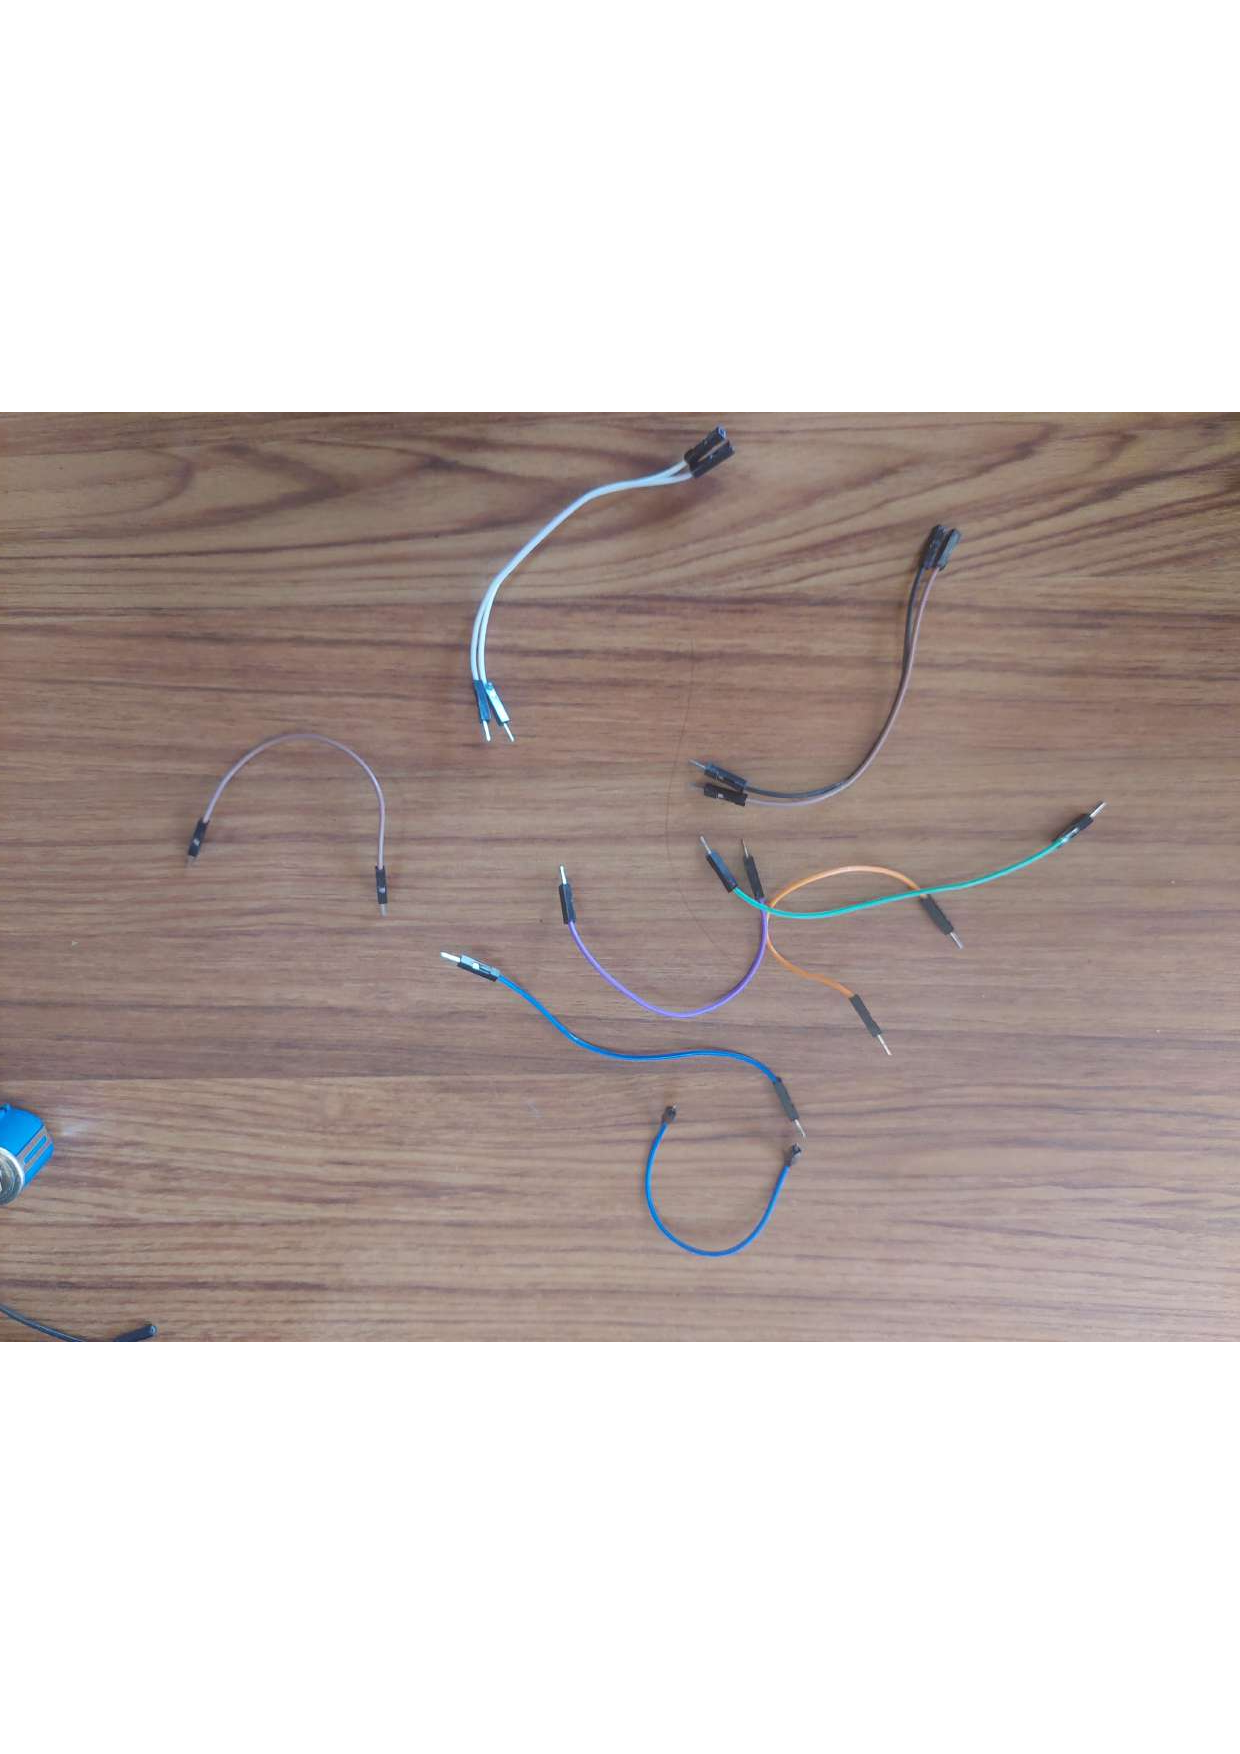
\includegraphics[trim = {1mm 1mm 1mm 1mm},clip,scale=0.2]{8/Img/Img/Cables dupont.pdf}
        \caption{Cables dupont}
        \label{Cables dupont}
    \end{figure}
    
    \begin{figure}[H]
        \centering
        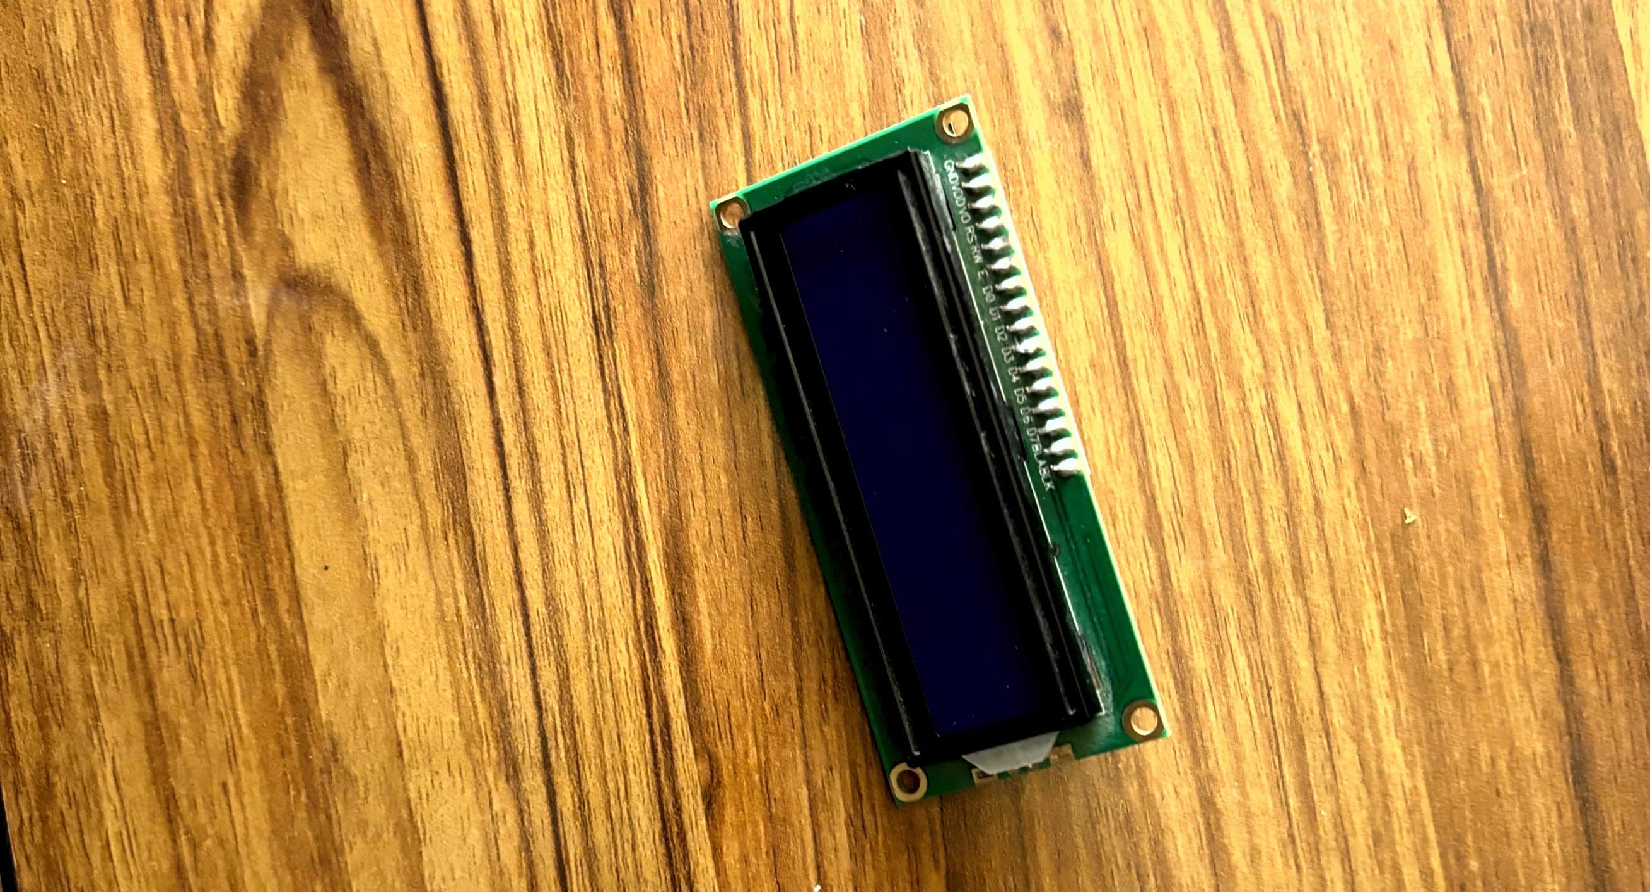
\includegraphics[trim = {80mm 1mm 60mm 1mm},clip,scale=0.2]{8/Img/Img/Display.pdf}
        \caption{Display}
        \label{Display}
    \end{figure}
    
    \begin{figure}[H]
        \centering
        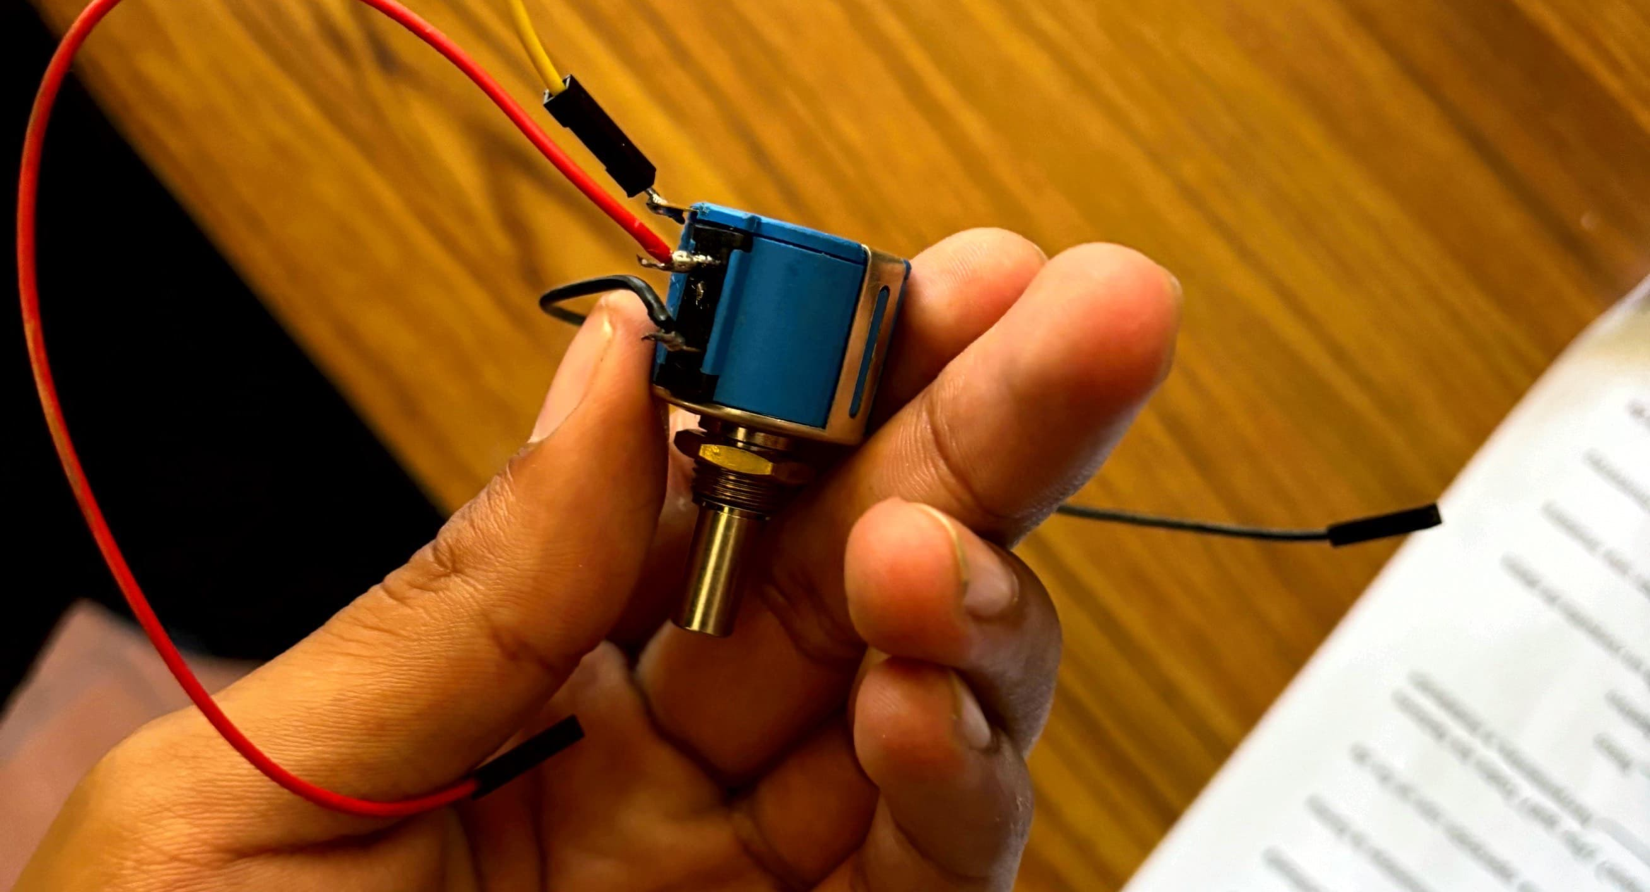
\includegraphics[trim = {70mm 1mm 70mm 1mm},clip,scale=0.2]{8/Img/Img/Potenciometro.pdf}
        \caption{Potenciómetro}
        \label{potenciometro}
    \end{figure}
    
    \begin{figure}[H]
        \centering
        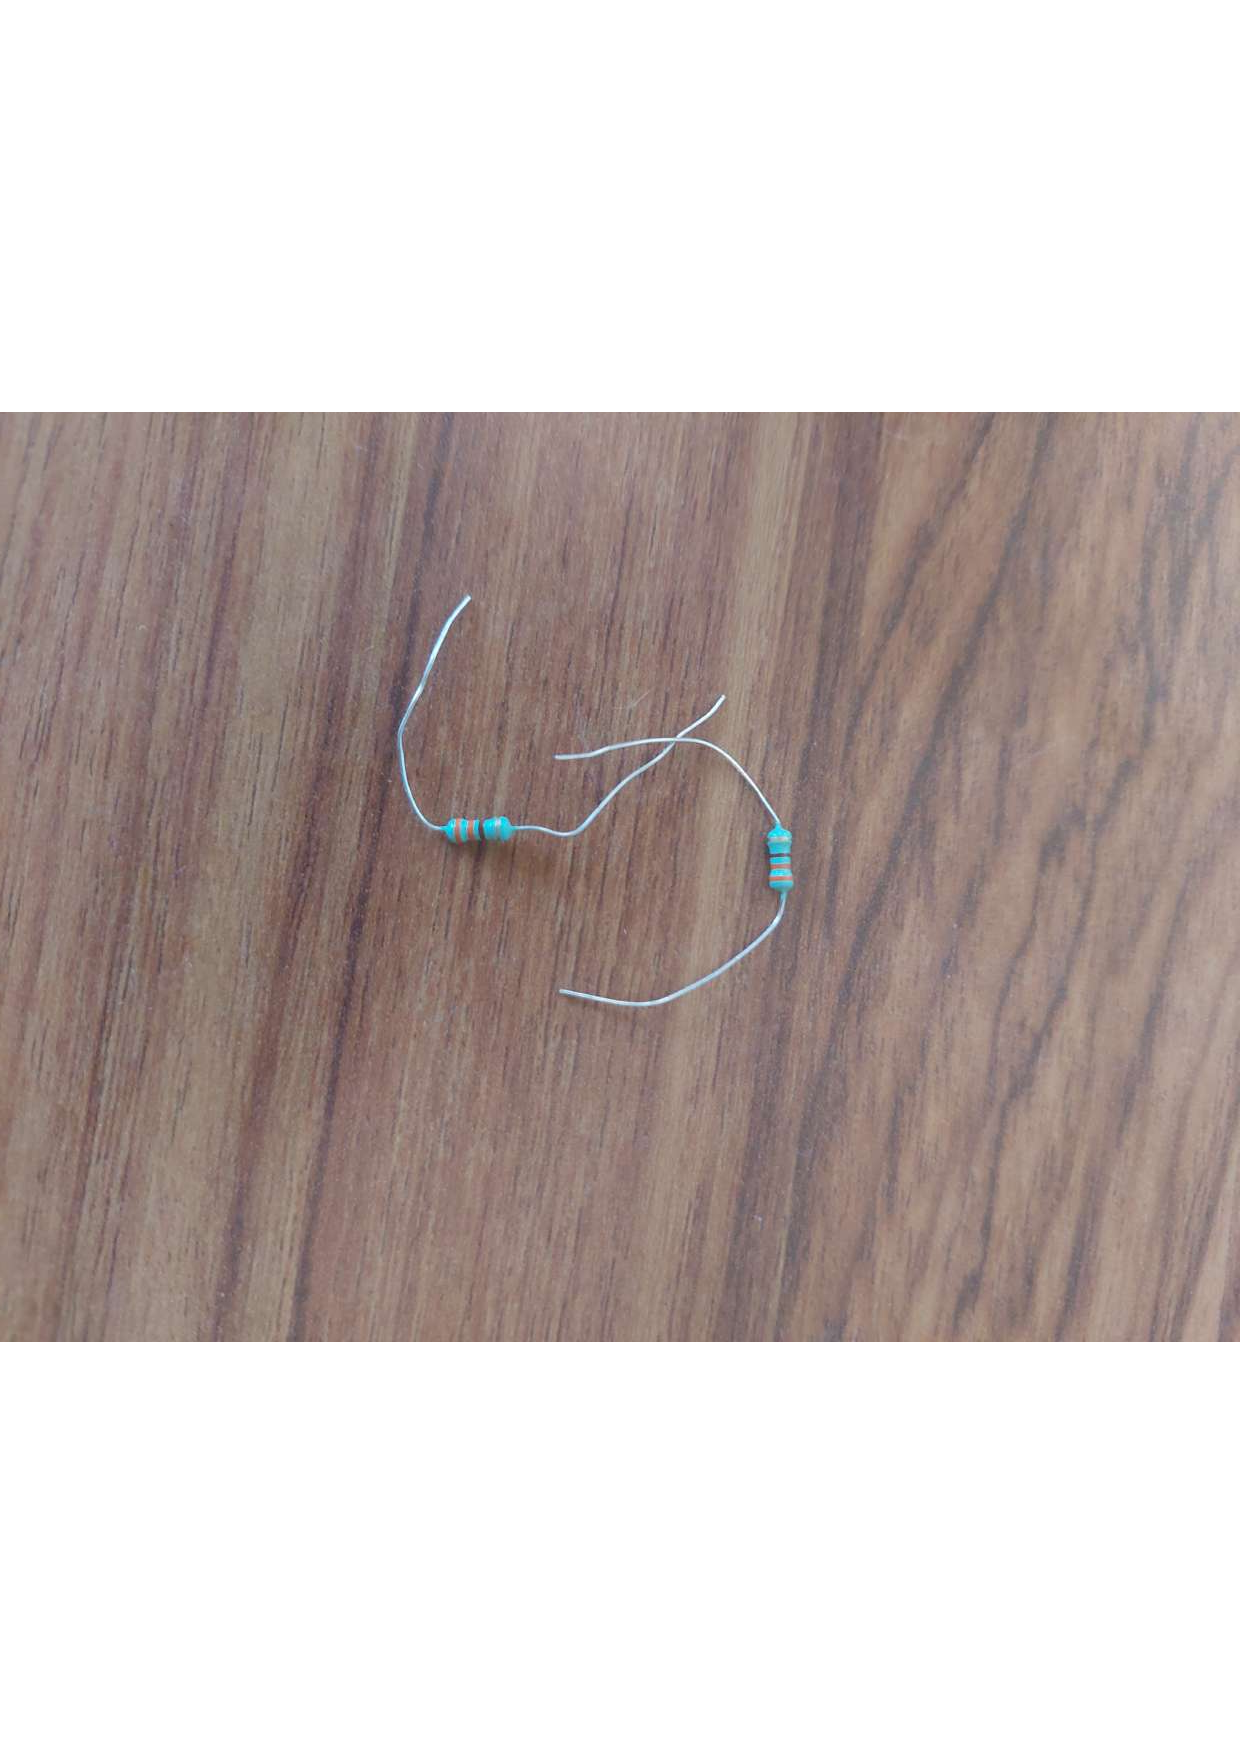
\includegraphics[trim = {30mm 1mm 30mm 1mm},clip,scale=0.2]{8/Img/Img/Resistencias.pdf}
        \caption{Resistencias}
        \label{Resistencias}
    \end{figure}
    
    \begin{figure}[H]
        \centering
        \includegraphics[trim = {30mm 30mm 30mm 10mm},clip,scale=0.2]{8/Img/Img/Cable usb.pdf}
        \caption{Cable usb}
        \label{Cable usb}
    \end{figure}
    
    \begin{figure}[H]
        \centering
        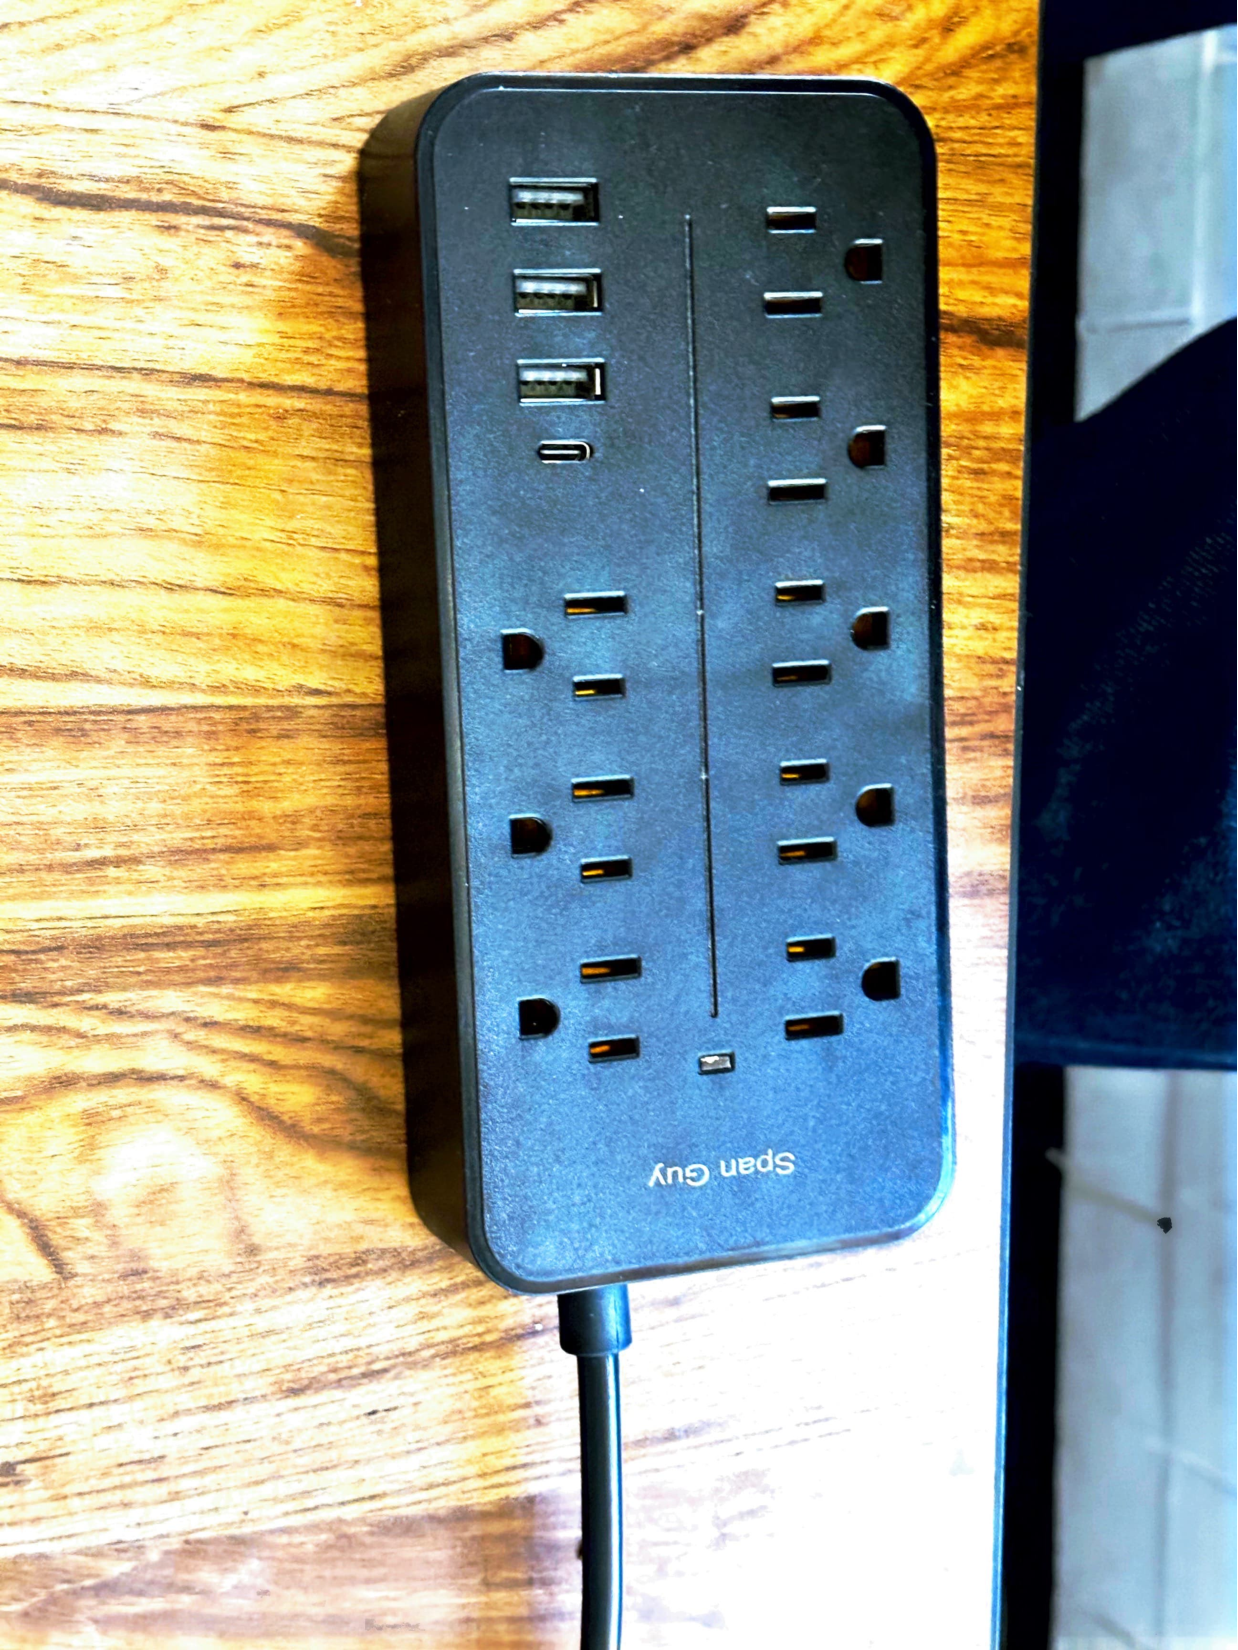
\includegraphics[trim = {30mm 30mm 30mm 10mm},clip,scale=0.2]{8/Img/Img/Multicontacto.pdf}
        \caption{Multicontacto}
        \label{Multicontacto}
    \end{figure}
    
    \begin{figure}[H]
        \centering
        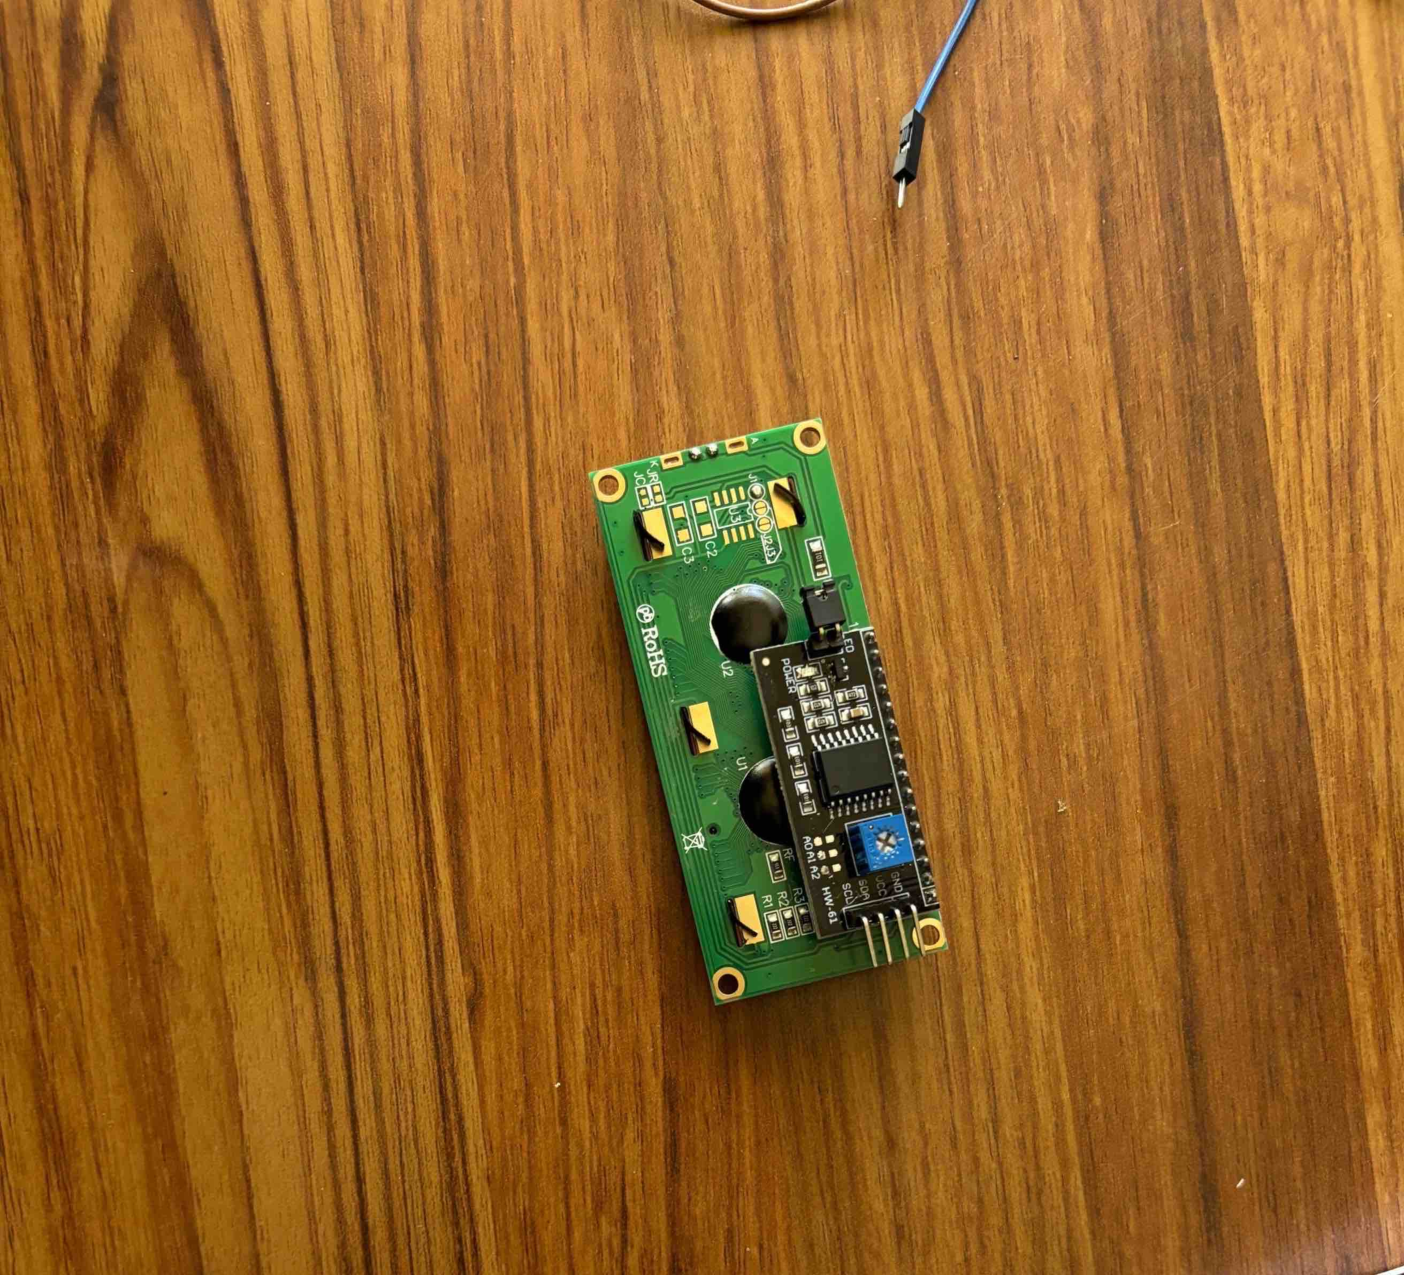
\includegraphics[trim = {60mm 20mm 60mm 60mm},clip,scale=0.2]{8/Img/Img/Modulo adaptador.pdf}
        \caption{Modulo adaptador}
        \label{Modulo adaptador}
    \end{figure}
    
    \begin{figure}[H]
        \centering
        \includegraphics[trim = {1mm 1mm 1mm 1mm},clip,scale=0.2]{8/Img/Img/SP32.pdf}
        \caption{SP32}
        \label{SP32}
    \end{figure}
    
    \begin{figure}[H]
        \centering
        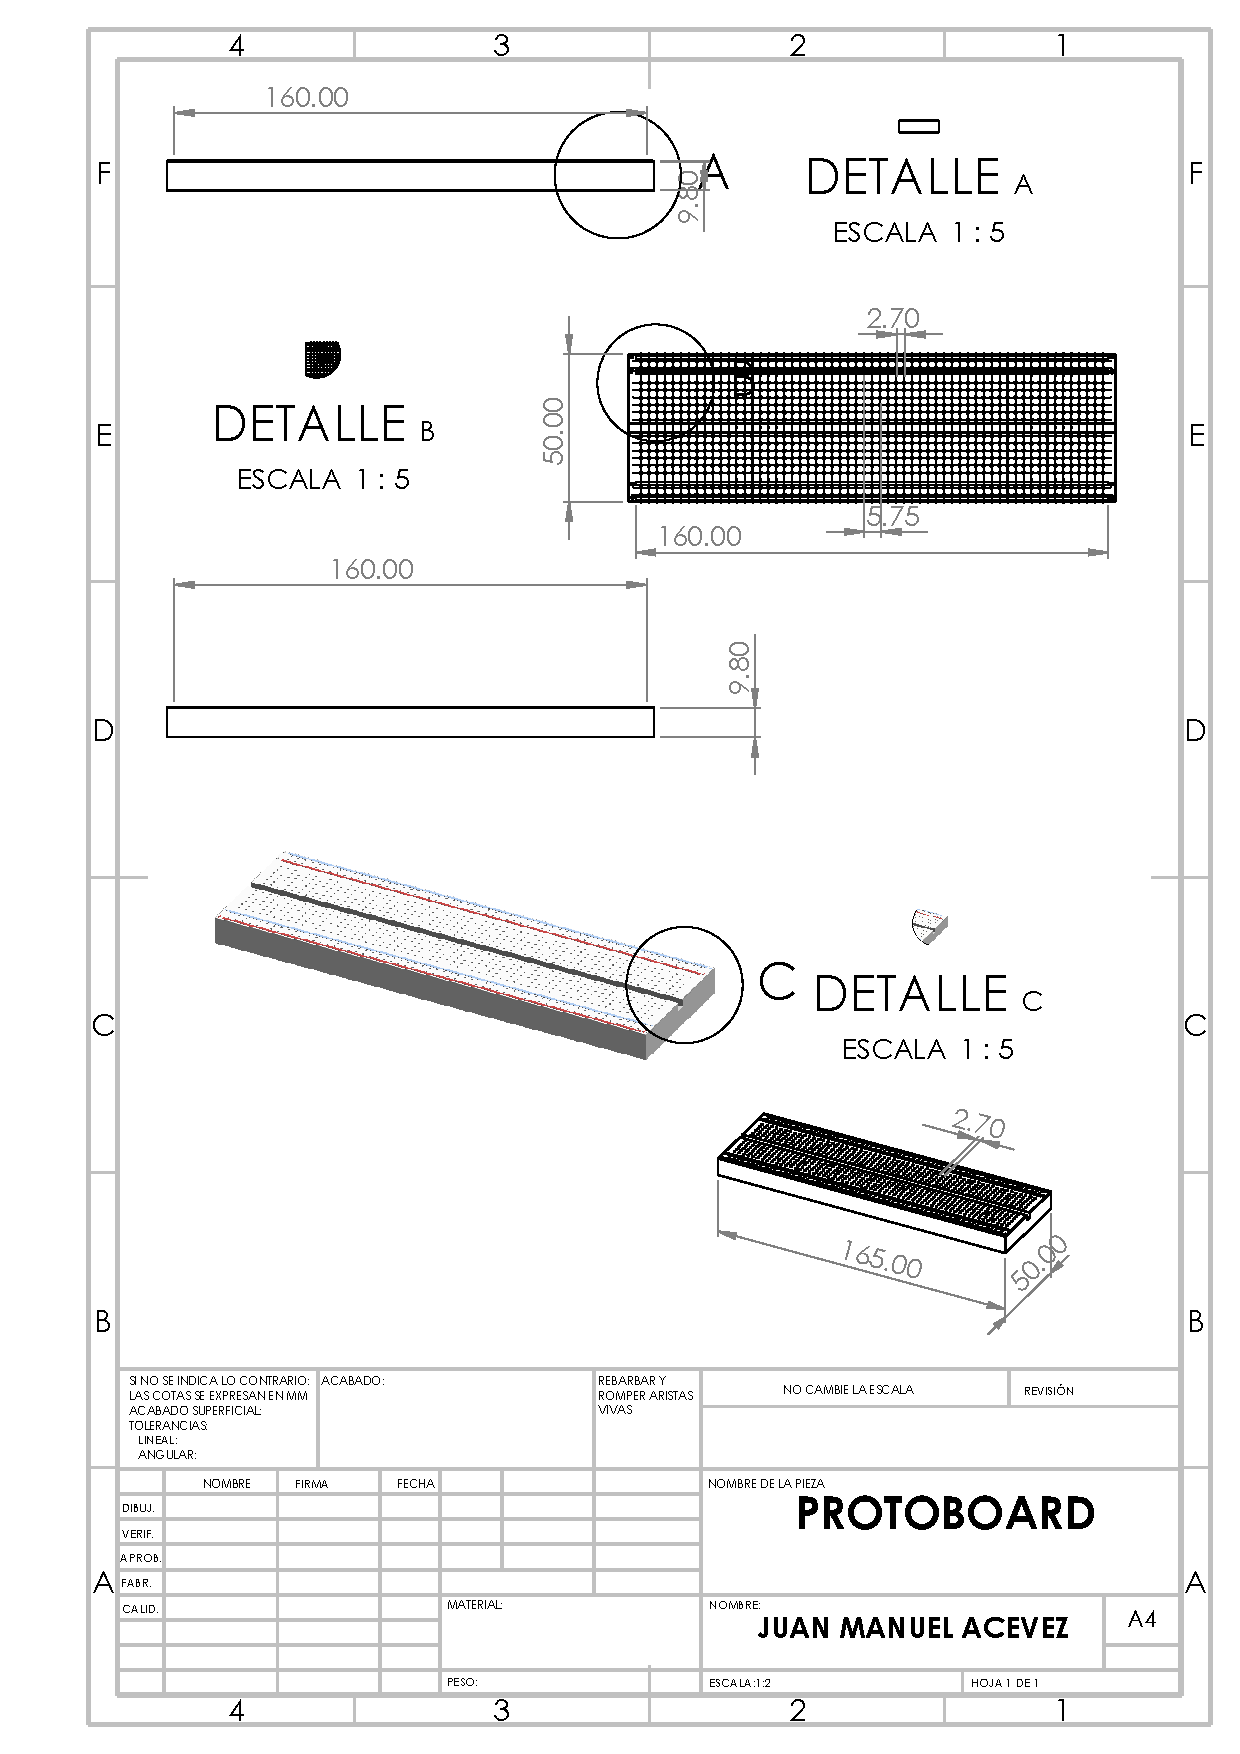
\includegraphics[trim = {40mm 20mm 20mm 20mm},clip,scale=0.2]{8/Img/Img/Protoboard.pdf}
        \caption{Protoboard}
        \label{Protoboard}
    \end{figure}
    
    \begin{figure}[H]
        \centering
        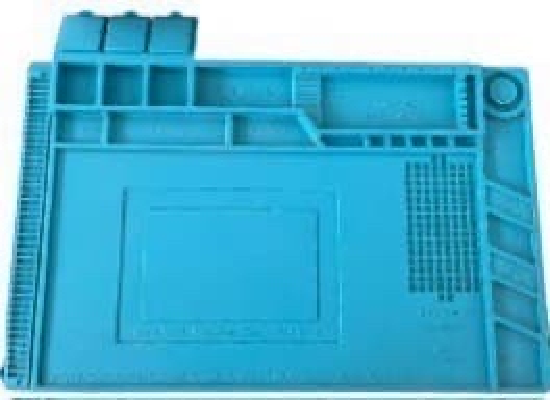
\includegraphics[trim = {1mm 1mm 1mm 1mm},clip,scale=0.6]{8/Img/Img/Tapete silicon.pdf}
        \caption{Silicon}
        \label{Siliconl}
    \end{figure}
    
    \begin{figure}[H]
        \centering
        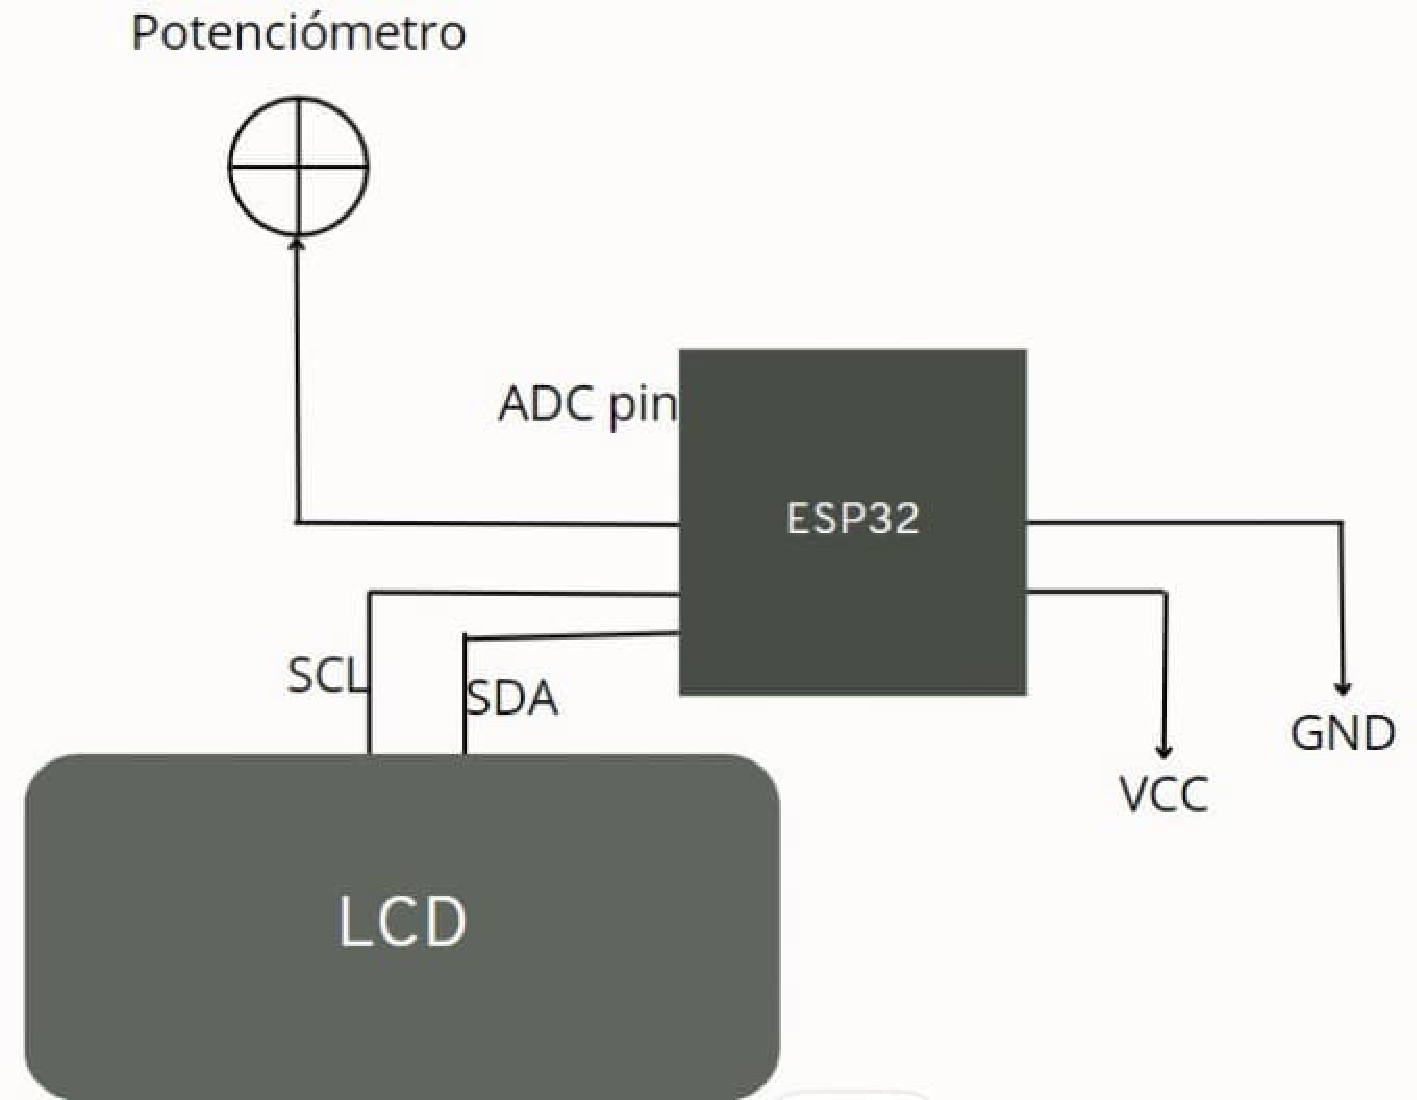
\includegraphics[trim = {1mm 1mm 1mm 1mm},clip,scale=0.3]{8/Img/Img/Cadena de medida.pdf}
        \caption{Cadena de medida}
        \label{Cadena de medida}
    \end{figure}
    
    \begin{figure}[H]
        \centering
        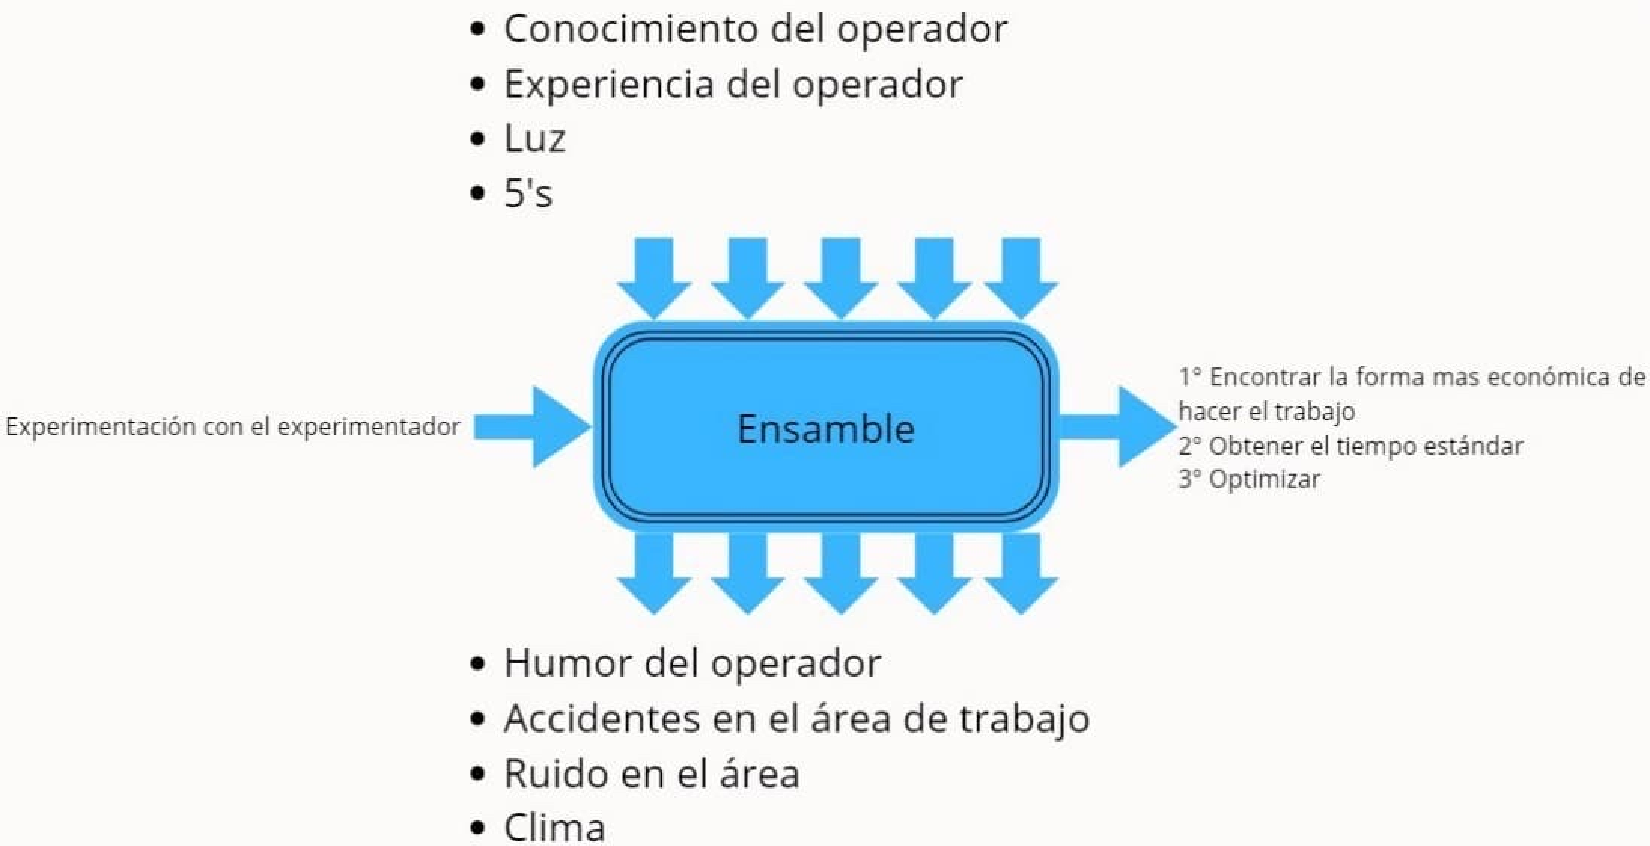
\includegraphics[trim = {1mm 1mm 1mm 1mm},clip,scale=0.3]{8/Img/Diagrama de entradas y salidas.pdf}
        \caption{Diagrama de entradas y salidas}
        \label{Diagrama de entradas y salidas}
    \end{figure}
    
    
    \begin{itemize}
        \item Se debe establecer que se habrá de hacer, como, conque, y donde para obtener la información que permita probar la hipótesis.  
        \item Se debe desglosar de acuerdo a los objetivos específicos. 
        \item Se debe establecer una estrategia metodológica por cada objetivo específico. De manera simplista se podría decir que se cambia el verbo en infinitivo por su respectivo adverbio.
        \item En cada objetivo se debe describir que método, que materiales y que equipo se usará para conseguirlo.
    \end{itemize}
    % 
    % 
    \subsection{Desarrollo de la guía de plan de Emergencia}
    
    El Plan de Emergencia: Documento que describe los lineamientos a seguir, la organización y los mecanismos, que indican la manera de enfrentar una situación de emergencia o desastre tanto en lo general como en lo particular, así como la utilización viable de los recursos humanos y materiales con los que se cuenta.
    % 
    % 
    \subsection{Análisis de los métodos, materiales, herramientas e instalación utilizada en la ejecución del ensamble de un circuito electrónico}
    
    \subsubsection{Planeación}
    Para realizar el trabajo se deberá tener un conocimiento a partir de las clases de lo que es el estudio de movimientos y tiempos además de tiempos ciclos y estándar, para llevar a cabo el ensamble se necesitará que el analista realice un manual para que el operador pueda llevar a cabo el ensamble \ref{Ensamble}.
    Posterior a eso debemos planificar como se usara el material y tener conocimiento sobre este para eso se hizo una tabla\ref{Material}.
    Al realizar el trabajo en parejas se deberá asignar las horas y el día que se lo usara cada quien para que todos alcancen a grabar sus 2 pruebas, mi compañera y yo decidimos comprar una ESP32 al profesor ya que haría un pedido de ESP32 esto con el fin de que cada quien pueda trabajar con la suya y no afecte a los demás a la hora de querer realizar sus ensambles ya que llego un punto en el que se retraso el trabajo debido a que compañeros que iniciaron con sus ensambles terminaron quemando la ESP32 viéndonos afectados los demás ya que nos quedamos sin el material necesario para llevar a cabo la operación, la compra de la ESP32 presento un gasto que se sumo a la compra de otros materiales como fueron resistencias y cables dupont, sin embargo este gasto no se ve como perdida sino como una inversión con el fin de reducir retrasos ya que nadie ajeno a nosotros podrá manipular nuestros materiales y podremos llevar a cabo sin retrasos el ensamble  en el tiempo establecido.
    % 
    % 
    \subsubsection{5's}
     Para realizar el ensamble podemos hacer uso de varias metodologías como lo pueden ser las 5's las cuales tienen como propósito mantener y mejorar las condiciones de organización, orden y limpieza, así como mejorar las condiciones de trabajo, seguridad, clima laboral, motivación personal y eficiencia.
    Algunas de las 5's que podemos utilizar son la clasificación y orden, estas nos ayudaran para eliminar lo innecesario reduciendo el desorden con el fin de facilitar el acceso a las herramientas y hacer mas eficiente el trabajo, así como también podemos usar la estandarización la cual va de la mano de las metodologías que nosotros buscamos usar como lo es el estudio de movimientos y tiempos.
    %
    % 
    \subsubsection{Desarrollo del sistema de tiempos predeterminado}
    Son una colección de tiempos de movimientos básicos. Se asignan a los movimientos fundamentales y a grupos de movimientos que no es posible evaluar con precisión mediante los procedimientos normales de estudio de tiempos con cronometro. Son resultado del estudio de una muestra grande de diversas operaciones con un dispositivo de tiempos como una cámara de película o de vídeo-grabación capaz de medir elementos muy cortos.
    \cite{Sistemadetiempospredeterminados}
    % 
    % 
    \subsubsection{Desarrollo del muestreo del trabajo}
    Paso 1: Selecciona las actividades o actividad a observar y socializa
    Paso 2: Calcular la proporción del tiempo de la actividad o demora (p)
    Paso 3: Calcular el número de observaciones con la exactitud deseada y el valor de z
    Paso 4: Cómo determinar la frecuencia de las observaciones
    Paso 5: Observar y registrar las actividades
    Paso 6: Analizar los resultados
    \cite{muestreodeltrabajo}
    %
    % 
    \subsubsection{Corrección por balanceo de procesos}
    El balanceo de línea ayudará a determinar si se cuentan con los recursos necesarios para iniciar una nueva línea de producción o hacen falta elementos para cubrirla. Encontrar el balance en una empresa va de la mano con esta metodología, en la que cada pieza es fundamental para completar el engranaje final.
    \cite{Balanceodelineas}
    % 
    % 
    \subsubsection{Datos estándar continuos y discretos}
    Si las observaciones corresponden a cantidades, las variables pueden distinguirse entre discretas y continuas. Se dice que una variable es discreta cuando no puede tomar ningún valor entre dos consecutivos, y que es continua cuando puede tomar cualquier valor dentro de un intervalo.
    \cite{Datoscontinuosydiscretos}
    %
    % 
    \begin{figure}[H]
        \centering
        \includegraphics[trim = {1mm 1mm 1mm 1mm},clip,scale=0.3]{8/Img/SP32.pdf}
        \caption{Cotas de la SP32}
        \label{Cotas SP32}
    \end{figure}
    
    
    \begin{figure}[H]
        \centering
        \includegraphics[trim = {1mm 1mm 1mm 1mm},clip,scale=0.3]{8/Img/cabledupont.pdf}
        \caption{Cotas cable dupont}
        \label{Cotas Cable dupont}
    \end{figure}
    
    
    
    \begin{figure}[H]
        \centering
        \includegraphics[trim = {1mm 1mm 1mm 1mm},clip,scale=0.3]{8/Img/display.pdf}
        \caption{Cotas display}
        \label{Cotas display}
    \end{figure}
    
    
    \begin{figure}[H]
        \centering
        \includegraphics[trim = {1mm 1mm 1mm 1mm},clip,scale=0.3]{8/Img/moduloAdaptadorLcd.pdf}
        \caption{Cotas modulo adaptador}
        \label{Cotas modulo adapatdor}
    \end{figure}
    
    
    \begin{figure}[H]
        \centering
        \includegraphics[trim = {1mm 1mm 1mm 1mm},clip,scale=0.3]{8/Img/multicontacto.pdf}
        \caption{Cotas multicontacto}
        \label{Cotas multicontacto}
    \end{figure}
    
    
    \begin{figure}[H]
        \centering
        \includegraphics[trim = {1mm 1mm 1mm 1mm},clip,scale=0.3]{8/Img/potenciometro1.pdf}
        \caption{Cotas potenciómetro}
        \label{Cotas potenciometro}
    \end{figure}
    
    
    \begin{figure}[H]
        \centering
        \includegraphics[trim = {1mm 1mm 1mm 1mm},clip,scale=0.3]{8/Img/protoboard1.pdf}
        \caption{Cotas protoboard}
        \label{Cotas protoboard}
    \end{figure}
    
    
    \begin{figure}[H]
        \centering
        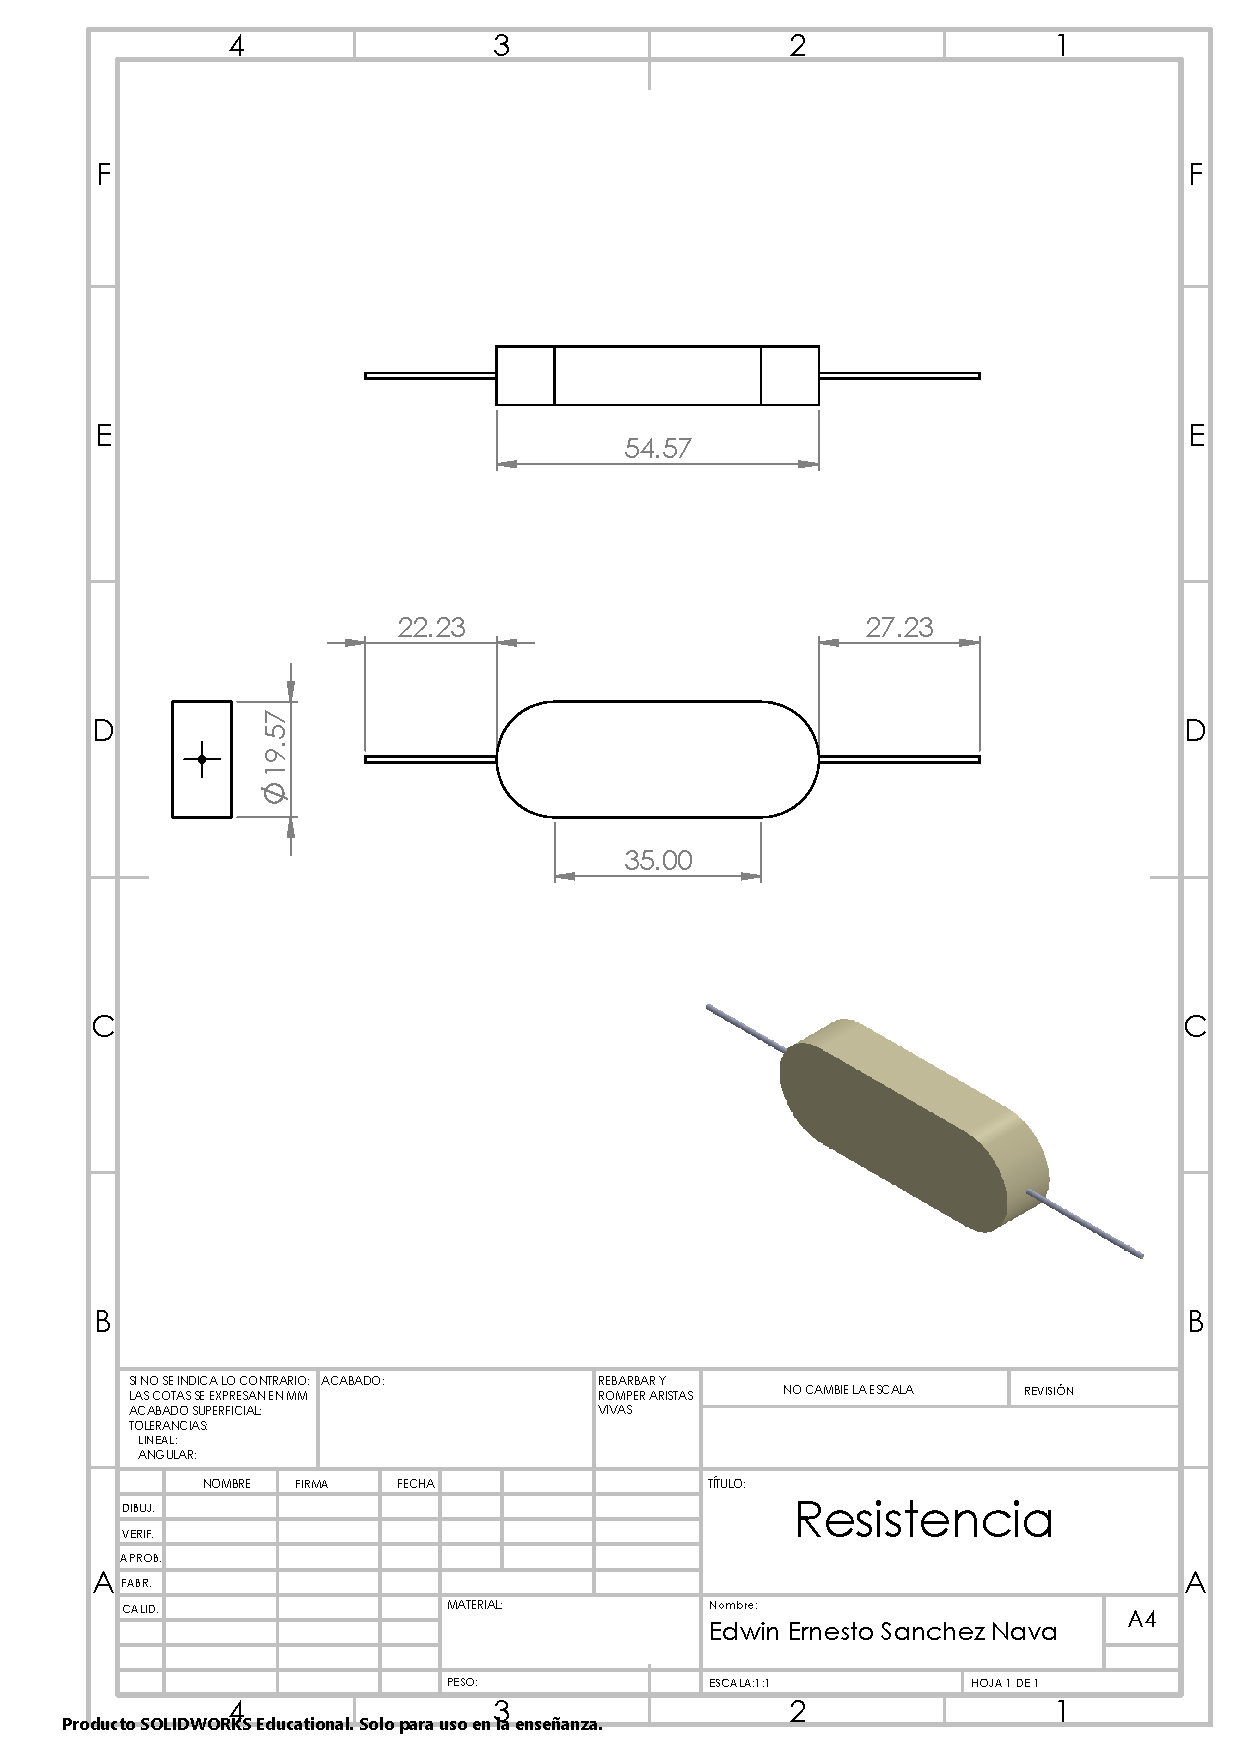
\includegraphics[trim = {1mm 1mm 1mm 1mm},clip,scale=0.3]{8/Img/resistencia.pdf}
        \caption{Cotas resistencia}
        \label{Cotas resistencia}
    \end{figure}
    %
    %
    \subsection{Diseño de la forma más económica de realizar el trabajo}
    
    % 
    % 
    \subsection{Normalización de los métodos, materiales, herramientas e instalaciones}
    
    % 
    % 
    \subsection{Determinación del tiempo estándar para que una persona competente realice el trabajo con marcha normal}
    
    % 
    % 
    % \subsection{Acrónimos y Abreviaciones}
    
    % Los acrónimos y abreviaciones deberán ser definidos únicamente la primera vez que aparecen en el texto, esto para que el lector entienda lo que significan.
    
    % \subsection{Ecuaciones}
    
    % Las ecuaciones son una excepción a las especificaciones prescritas de esta plantilla. 
    % Deberá determinar si su ecuación debe escribirse o no utilizando la fuente Adobe Devangari. 
    % Para crear ecuaciones multinivel, puede ser necesario tratar la ecuación como un gráfico e insertarla en el texto después de aplicar el estilo de la platilla.
    % Las ecuaciones serán enumeradas de manera consecutiva, y el número de ecuación, entre paréntesis, se colocan al ras de la derecha, utilizando una tabulación derecha.
    % 
    % \begin{equation}
    %     \label{eq1}
    %     x + y = z 
    % \end{equation}
    % 
    % Es importante asegurarse de que los símbolos de la ecuación sean definidos antes o inmediatamente después de la ecuación. Utilice “(1)”, en vez de “Eq. 1” al enumerar las ecuaciones, excepto al principio de una oración: “La ecuación (\ref{eq1}) es…”
    
    \section{Resultados y discusión}
    
    \subsection{Desarrollo de la Guía plan de emergencia}
    Con esta guía buscamos disminuir en su totalidad las emergencias de riesgo de incendio, así como el riesgo de accidentes en la institución Instituto Tecnológico de Querétaro capacitando al personal una vez al año para que en caso de emergencia se tome la mejor decisión para salvaguardar la integridad física de clientes internos y externos, así como de las instalaciones de la empresa.
    %
    %
    \begin{figure}[H]
        \centering
        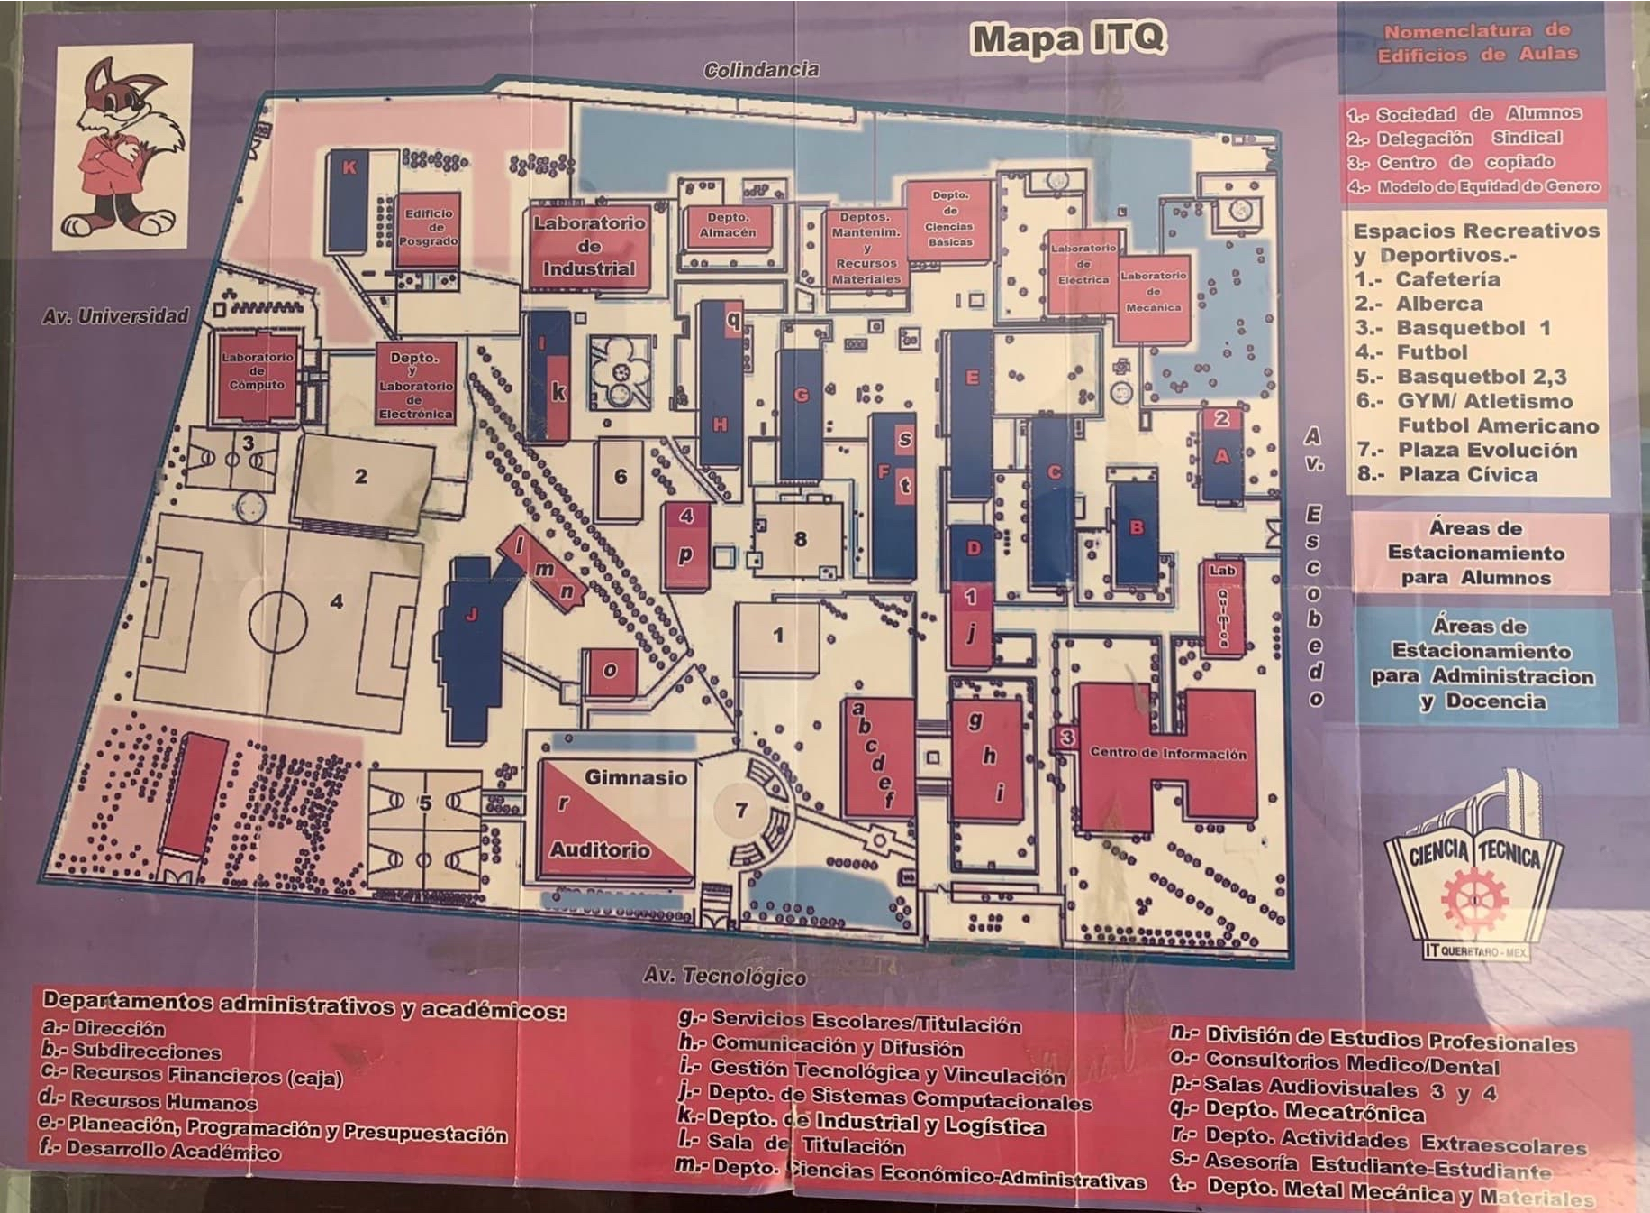
\includegraphics[trim = {1mm 1mm 1mm 1mm},clip,scale=0.3]{8/Img/Plano del ITQ.pdf}
        \caption{Tecnológico Nacional de México, Instituto Tecnológico de Querétaro, Av Tecnológico S/N, Centro Histórico, Centro, 76000, Querétaro, Qro., 4422274400 Ext. 4423}
        \label{Plano del ITQ}
    \end{figure}
    %
    %
    \begin{figure}[H]
        \centering
        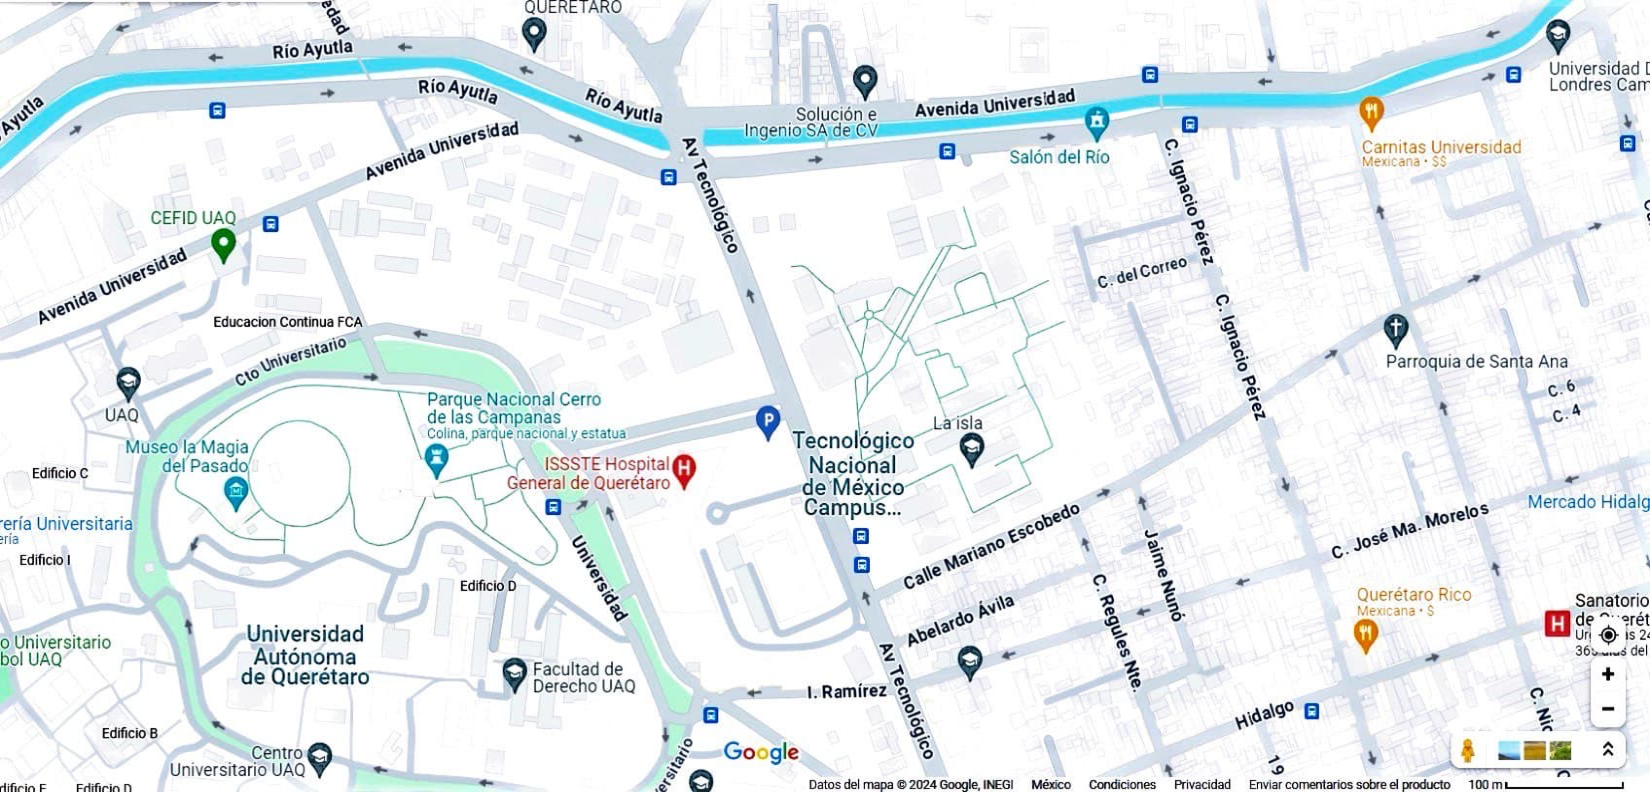
\includegraphics[trim = {1mm 1mm 1mm 1mm},clip,scale=0.3]{8/Img/Mapa Itq.pdf}
        \caption{Tecnológico Nacional de México, Instituto Tecnológico de Querétaro, Av Tecnológico S/N, Centro Histórico, Centro, 76000, Querétaro, Qro., 4422274400 Ext. 4423}
        \label{Mapa Itq}
    \end{figure}
    %
    %
    \begin{figure}[H]
        \centering
        \includegraphics[trim = {1mm 1mm 1mm 1mm},clip,scale=0.3]{8/Img/Plano edificio C.pdf}
        \caption{Plano del edificio donde se llevo a cabo el ensamble}
        \label{Edificio C}
    \end{figure}
    %
    %
    \begin{figure}[H]
        \centering
        \includegraphics[trim = {1mm 1mm 1mm 1mm},clip,scale=0.3]{8/Img/Cotas edificio C.pdf}
        \caption{Medidas del edificio C}
        \label{Cotas edifciio C}
    \end{figure}
    %
    %
    \subsubsection{Identificación del riesgo}
    Estamos comprometidos a mantener todos los días un programa interno de prevención de riesgos, así como una retroalimentación por parte de clientes internos y externos en los riesgos que se presentan en las actividades constantes por su parte invitamos a utilizar el equipo de trabajo.
    Evaluamos a cada riesgo interno por un rango para dar prioridad en las acciones véase Tabla
    %
    %
    \begin{figure}[H]
        \centering
        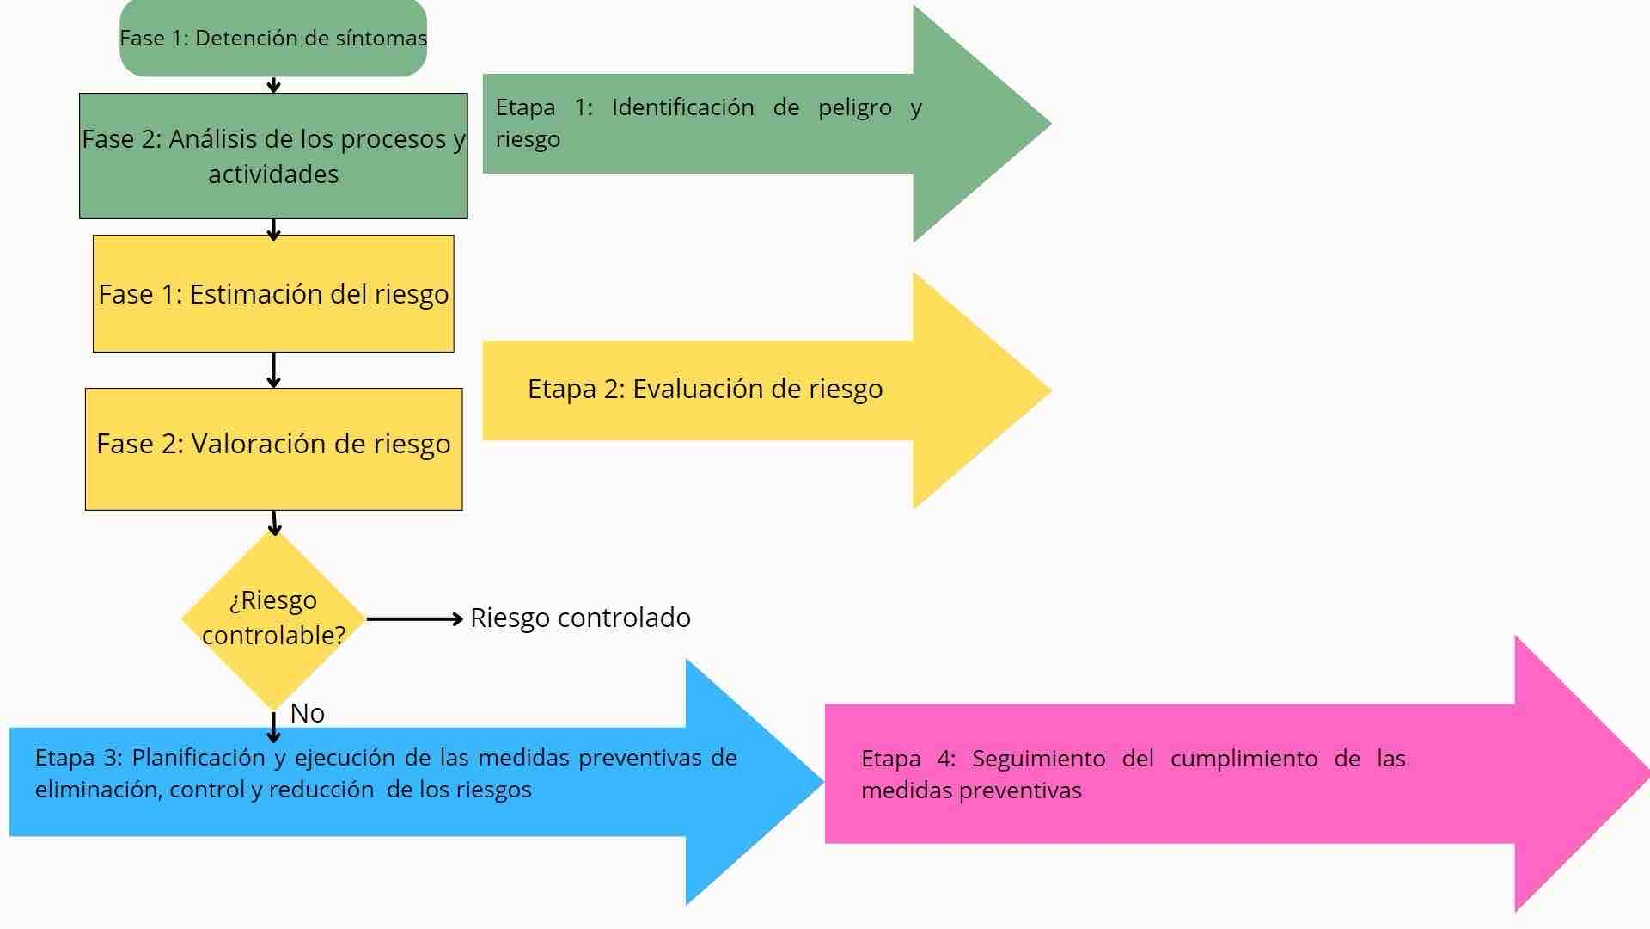
\includegraphics[trim = {1mm 1mm 1mm 1mm},clip,scale=0.3]{8/Img/Diagrama para la identiicacion de riesgos.pdf}
        \caption{Diagrama para la identificación de riesgos y acciones}
        \label{Diagrama para la identiicacion de riesgos}
    \end{figure}
    %
    %
    \subsubsection{Riesgos internos}
    
    El riesgo se define como la posibilidad de que algo suceda o no suceda en otras palabras es la proximidad de un daño. 
    El riesgo operativo interno lo definimos como la posibilidad de que sufre la empresa derivado de los fallos naturales en su propio funcionamiento.
    % 
    % 
    \begin{table}[h]
        \centering
        \caption{Riesgos con diferentes niveles y colores para distinguir la gravedad y acciones}
        \begin{tabular}{|c| c| c|}
        \hline
        \multicolumn{3}{|c|}{Riesgos}\\
        \hline
             Alto& 0.99 - 0.18 & Rojo  \\
        \hline     
             Medio& 0.17 - 0.05 & Amarillo \\
        \hline
             Bajo& 0.04 - 0.01 & Verde \\
        \hline
        \end{tabular}
        \label{tab:Riesgos}
    \end{table}
    % 
    % 
    \begin{figure}[H]
        \centering
        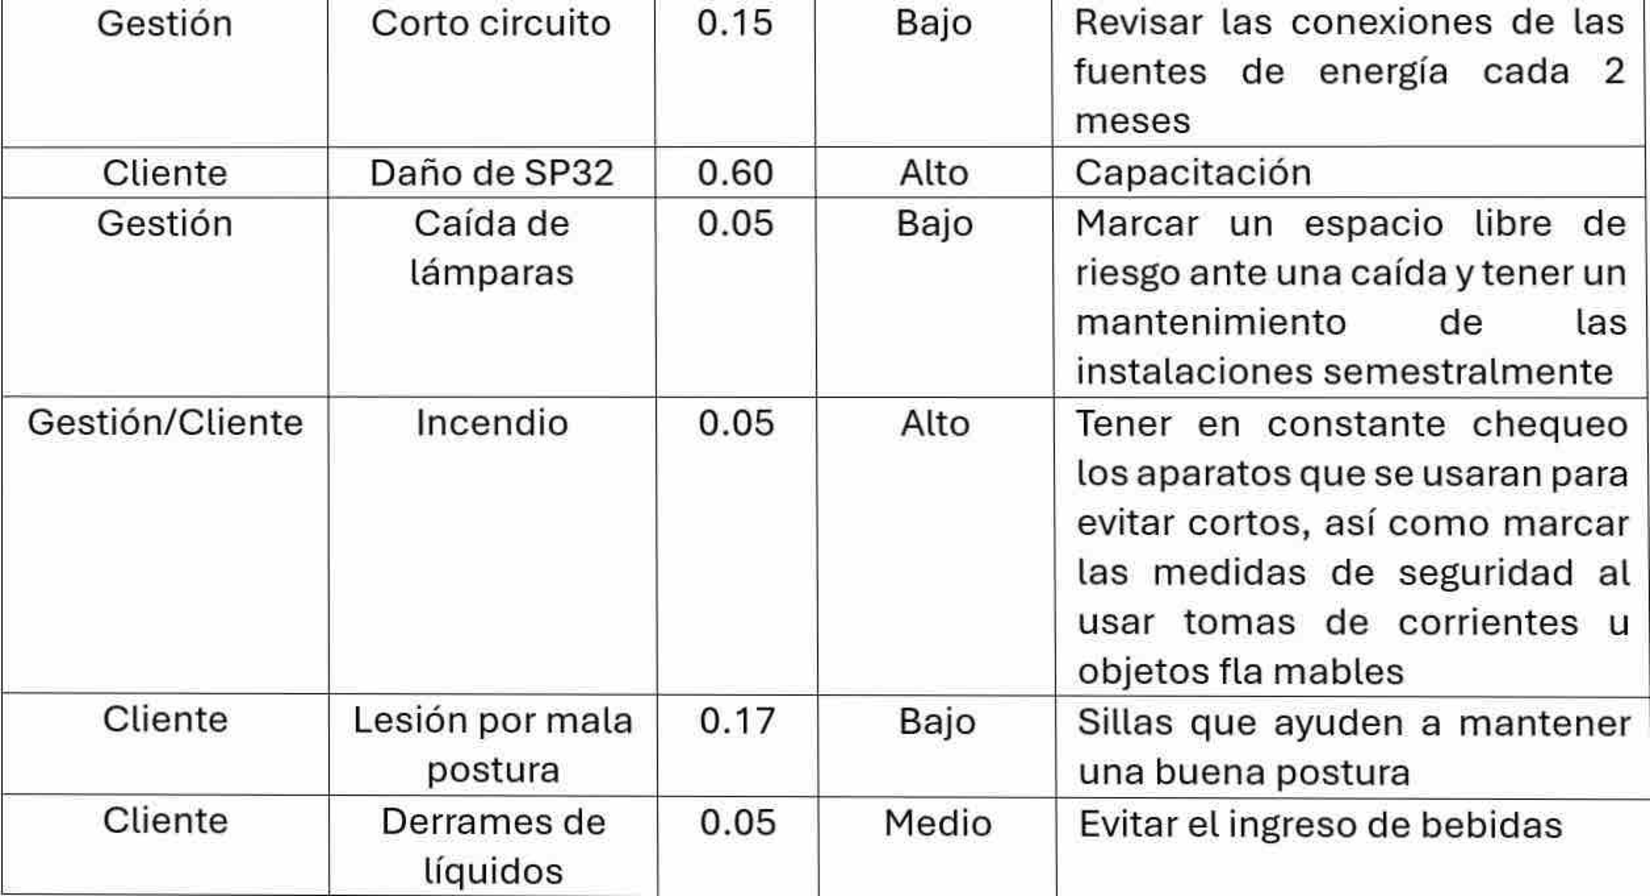
\includegraphics[trim = {1mm 1mm 1mm 1mm},clip,scale=0.3]{8/Img/Riesgos0.pdf}
        \caption{Descripción de los riesgos al realizar las actividades más comunes y de riesgo dentro de la empresa}
        \label{Riesgos internos}
    \end{figure}
    %
    %
    \subsubsection{Riesgos externos}
    
    \begin{figure}[H]
        \centering
        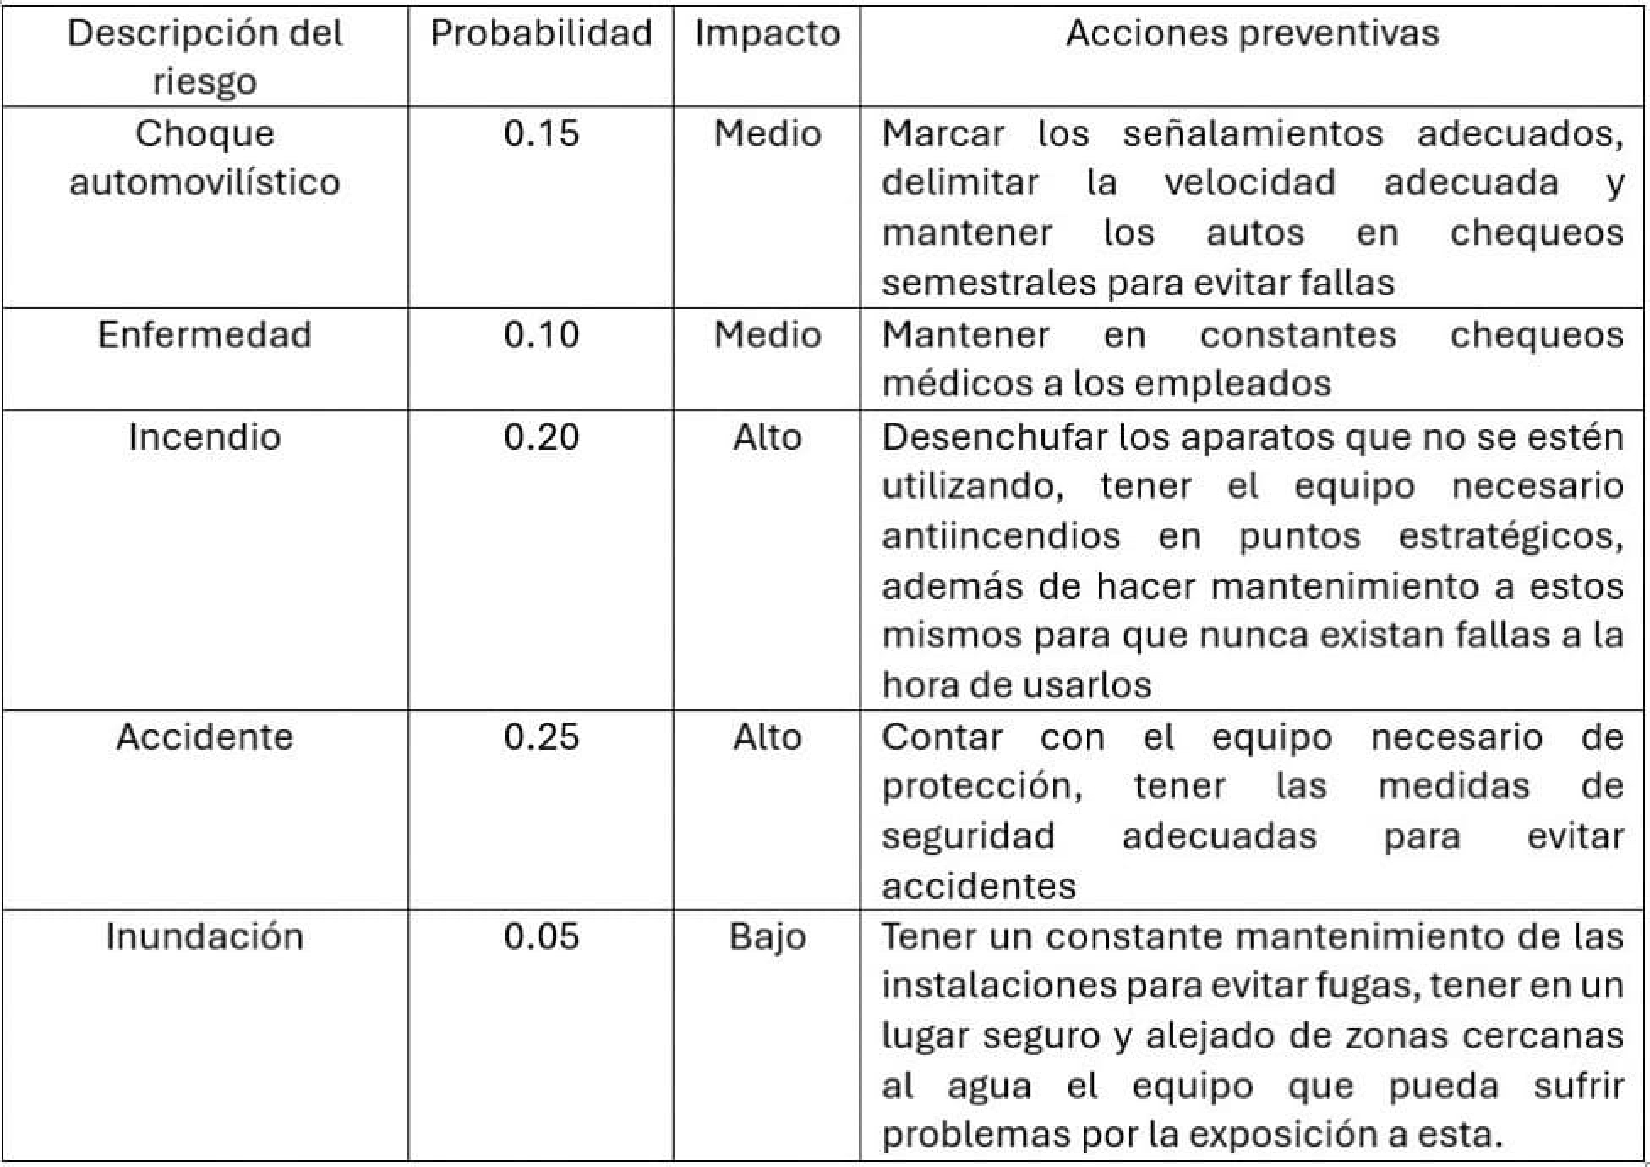
\includegraphics[trim = {1mm 1mm 1mm 1mm},clip,scale=0.3]{8/Img/Riesgos.pdf}
        \caption{Descripción de los riesgos externos}
        \label{Riesgos externos}
    \end{figure}
    %
    %
    \subsubsection{Programa de actividades de prevención y auxilio}
    
    Declaramos las diferentes acciones de lo que se piensa hacer cuando ocurra un riesgo interno u externo. 
    Las actividades de preparación y disposición que se hace anticipadamente en el ITP para evitar riesgos.
    % 
    % 
    \subsubsection{Plan de acción}
    
    Es el conjunto unitario de instrucciones que permite al ITQ realizar funciones diversas, como la resolución de problemas referentes a el manejo de riesgos internos y externos.
    % 
    % 
    % \begin{table}[H]
    %     \centering
    %     \caption{Descripción de las acciones anticipadas y correctivas ante un riesgo interno}
    %     \begin{tabular}{|p{5em}|p{10em}|p{11em}|p{10em}|}
    %         \hline
    %          RIESGO INTERNO& Acción Anticipada& Acción Correctiva& Indicador\\
    %          \hline
    %          Herida lacerada& Reemplazar las navajas y cuchillos por cutter con resorte. Utilizar en lo menos posible objetos punzo cortantes& Utilizar el material de los primeros auxilios y lavar la herida con agua oxigenada y vendar& Constancias de capacitación así como el registro de la disminución en el uso de curitas\\
    %          \hline
    %          Golpeo con martillo& Capacitación y descansos de 5 minutos cuando se este trabajando constantemente con el martillo& Aplicar pomada para golpes del botiquín de primeros auxilios& Menos reportes de golpes\\
    %          \hline
    %          Levantar super sacos& Capacitar con el uso adecuado de la faja y solicitar ayuda al momento de levantar materiales mayores a 30 kg& Tomar un descanso y tomar agua &Disminución del cansancio al final del día\\
    %          \hline
    %          Carga y descarga de camionetas& Capacitar con el uso adecuado de la faja y solicitar ayuda al momento de levantar materiales mayores a 30 kg& Utilizar más personal para evitar riesgos & Menor tiempo de carga y descarga en la camioneta\\
    %          \hline
    %          Chispa por cigarro& Señalamientos de no fumar a la entrada& Pedir de manera amable que apaguen el cigarro& Observar en el área de trabajo decremento de las colillas de cigarro\\
    %          \hline
    %          Corto circuito& Mantenimiento preventivo en los fusibles en el centro de carga& Bajar los interruptores del centro de carga& Obtención de un reporte técnico por lo menos una vez al año\\
    %          \hline
    %     \end{tabular}
    %     \label{tab:my_label}
    % \end{table}
    % 
    % 
    \begin{figure}[H]
        \centering
        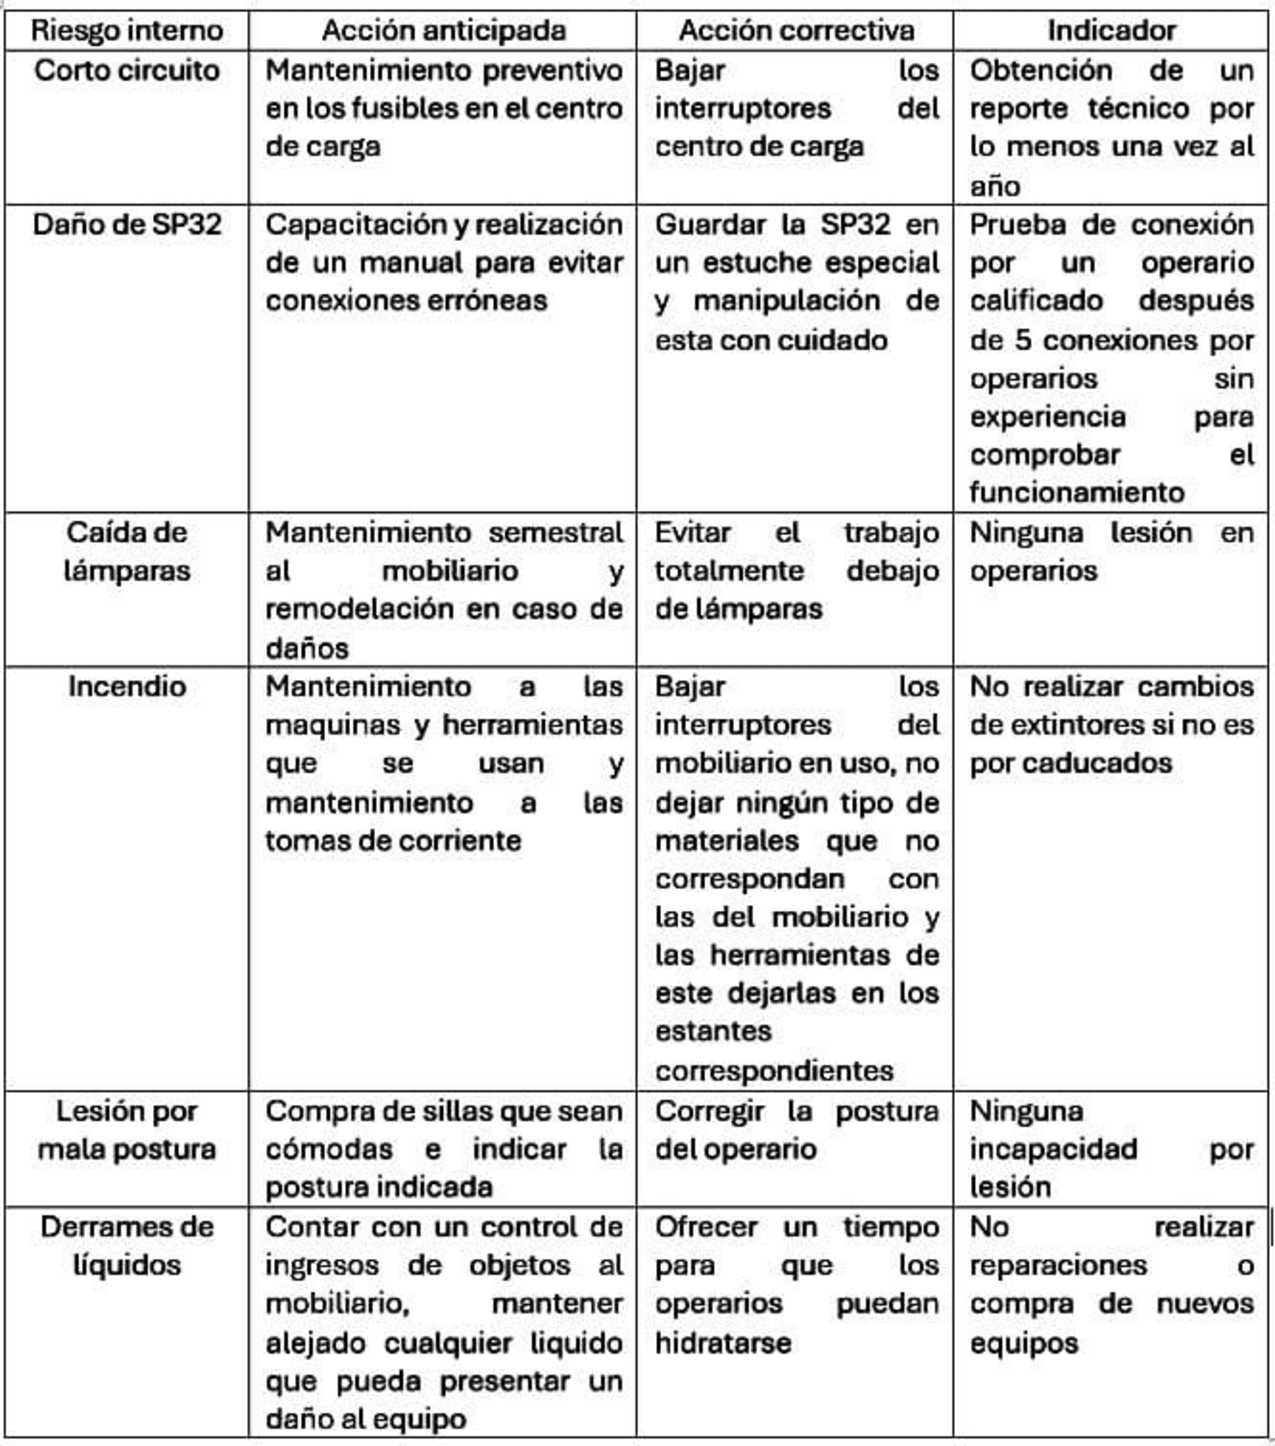
\includegraphics[trim = {1mm 1mm 1mm 1mm},clip,scale=0.3]{8/Img/Descripcion de las acciones anticipadas.pdf}
        \caption{Descripción de las acciones anticipadas y correctivas ante un riesgo interno}
        \label{DescripcionAntInterno}
    \end{figure}
    % 
    % 
    % \begin{table}[H]
    %     \centering
    %     \caption{Descripción de las acciones anticipadas y correctivas ante un riesgo externo e interno}
    %     \begin{tabular}{|p{5em}|p{10em}|p{11em}|p{10em}|}
    %          \hline
    %          RIESGO EXTERNO& Acción Anticipada& Acción Correctiva& Indicador\\
    %          \hline
    %          Desmayo del cliente& Tomar cursos de primeros auxilios por lo menos una vez al año a todo el personal& Contar con los conocimientos básicos de primeros auxilios& Realizar un simulacro que nos permita evaluar las acciones en el manejo del riesgo por desmayo\\
    %          \hline
    %          Incendio de algún vecino& Mantener los detectores de humo en lugares estratégicos y cambiar las pilas cada 2 meses& Llamar al 911 para informar del incendio y del posible riesgo en el negocio&  Llevar un registro de los cambios de las pilas en los detectores de humo\\
    %          \hline
    %          Incendio de camioneta& Mantener en mantenimiento los sensores de temperatura y con un extintor& Accionar el extintor conforme a lo establecido por el departamento de bomberos y llamar al 911& Revisar el tablero de la camioneta que no indique falta de agua o alta temperatura \\
    %          \hline
    %          Incendio por pirotecnia& Vigilar en los días festivos y mojar el material& Llamar a emergencias y tratar de sofocar el fuego& Hacer un llamado a los vecinos a ser cuidadosos\\
    %          \hline
    %          Choque en la avenida& Delimitar y poner conos de señalamiento& Llamar a emergencias y si es que hay daños a personas, aplicar primeros auxilios en caso de ser necesario& Llevar un registro de las horas pico para evitar hacer maniobras\\
    %          \hline
    %     \end{tabular}
    %     \label{tab:Acciones}
    % \end{table}
    % 
    % 
    \begin{figure}[H]
        \centering
        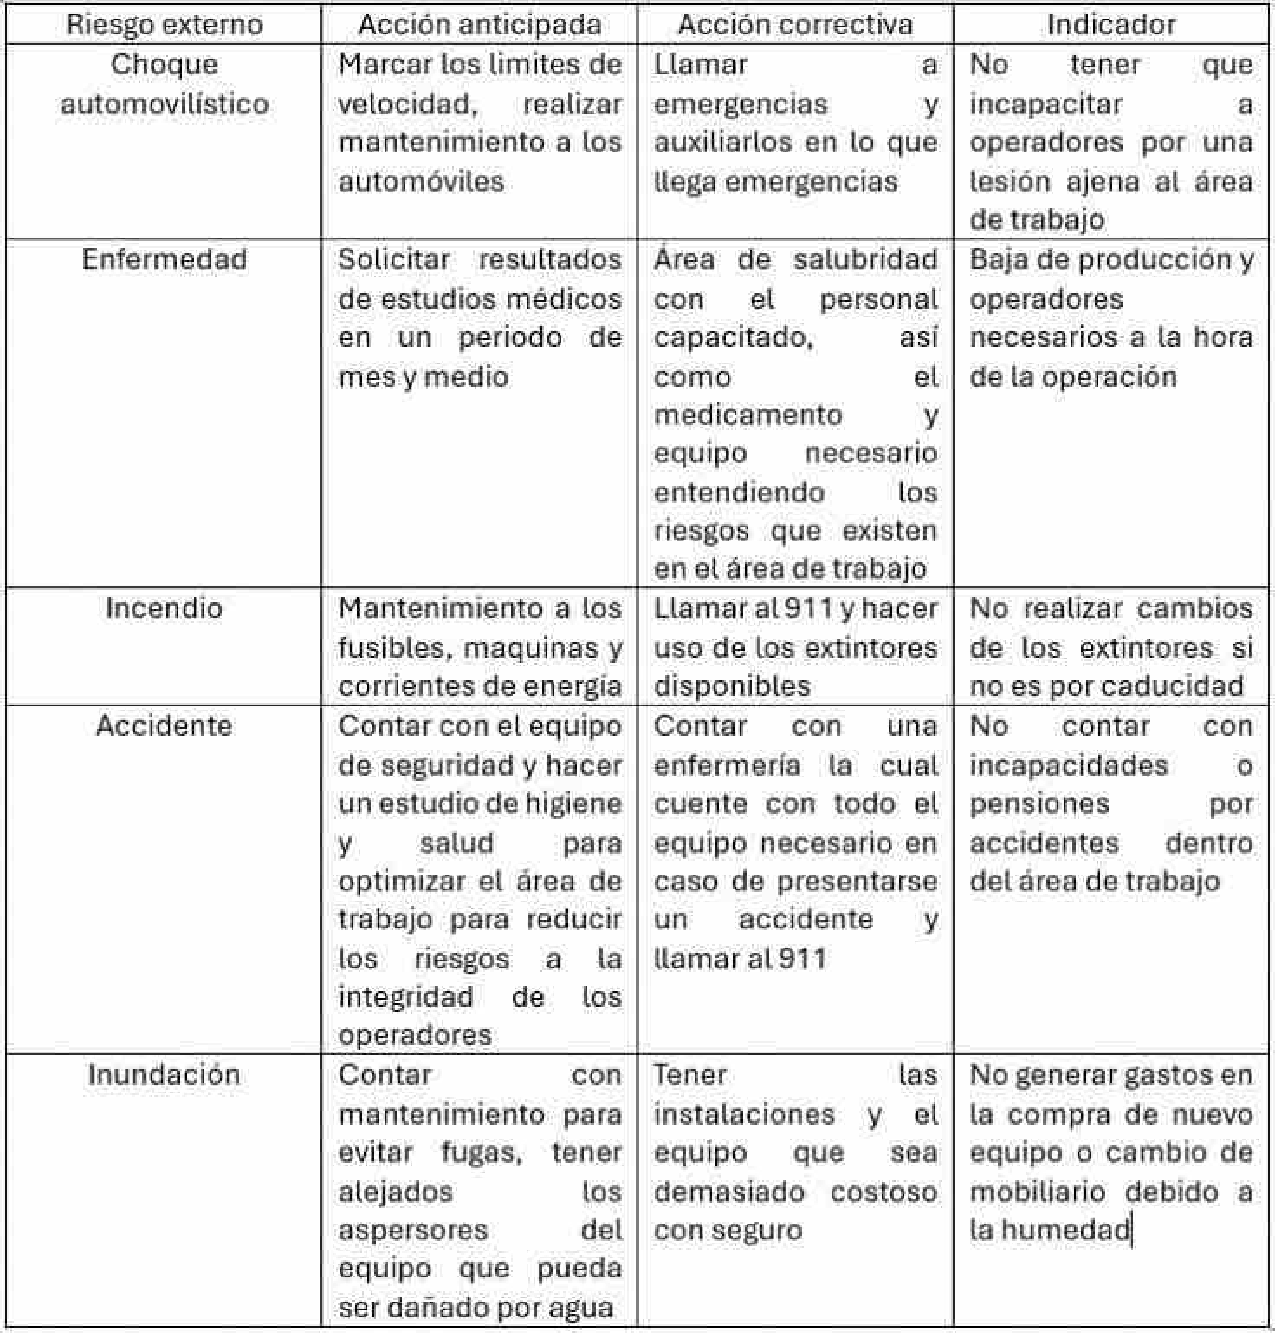
\includegraphics[trim = {1mm 1mm 1mm 1mm},clip,scale=0.3]{8/Img/Descripcion de acciones anticipadas.pdf}
        \caption{Descripción de las acciones anticipadas y correctivas ante un riesgo externo}
        \label{DescripcionAntExterno}
    \end{figure}
    % 
    % 
    % Cada estrategia metodológica se establece acorde a cada objetivo, y por tanto deberá ser desglosada precisada y ordenada claramente. En consecuencia cada objetivo que se presentó en forma de verbo en infinitivo deberá determinar una estrategia en forma de adverbio. Ej. Desarrollar…Desarrollo. Son las actividades ordenadas que tienen como finalidad la prueba de la hipótesis. 
    
    % \begin{itemize}
    %     \item Se debe establecer que se habrá de hacer, como, conque, y donde para obtener la información que permita probar la hipótesis.  
    %     \item Se debe desglosar de acuerdo a los objetivos específicos. 
    %     \item Se debe establecer una estrategia metodológica por cada objetivo específico. De manera simplista se podría decir que se cambia el verbo en infinitivo por su respectivo adverbio.
    %     \item En cada objetivo se debe describir que método, que materiales y que equipo se usará para conseguirlo.
    %     \item Se deben tener referencias Figura \ref{fig:lcd-16x2}.
    % \end{itemize}
    % 
    % 
    % \begin{figure}[H]
    %     \centering
    %     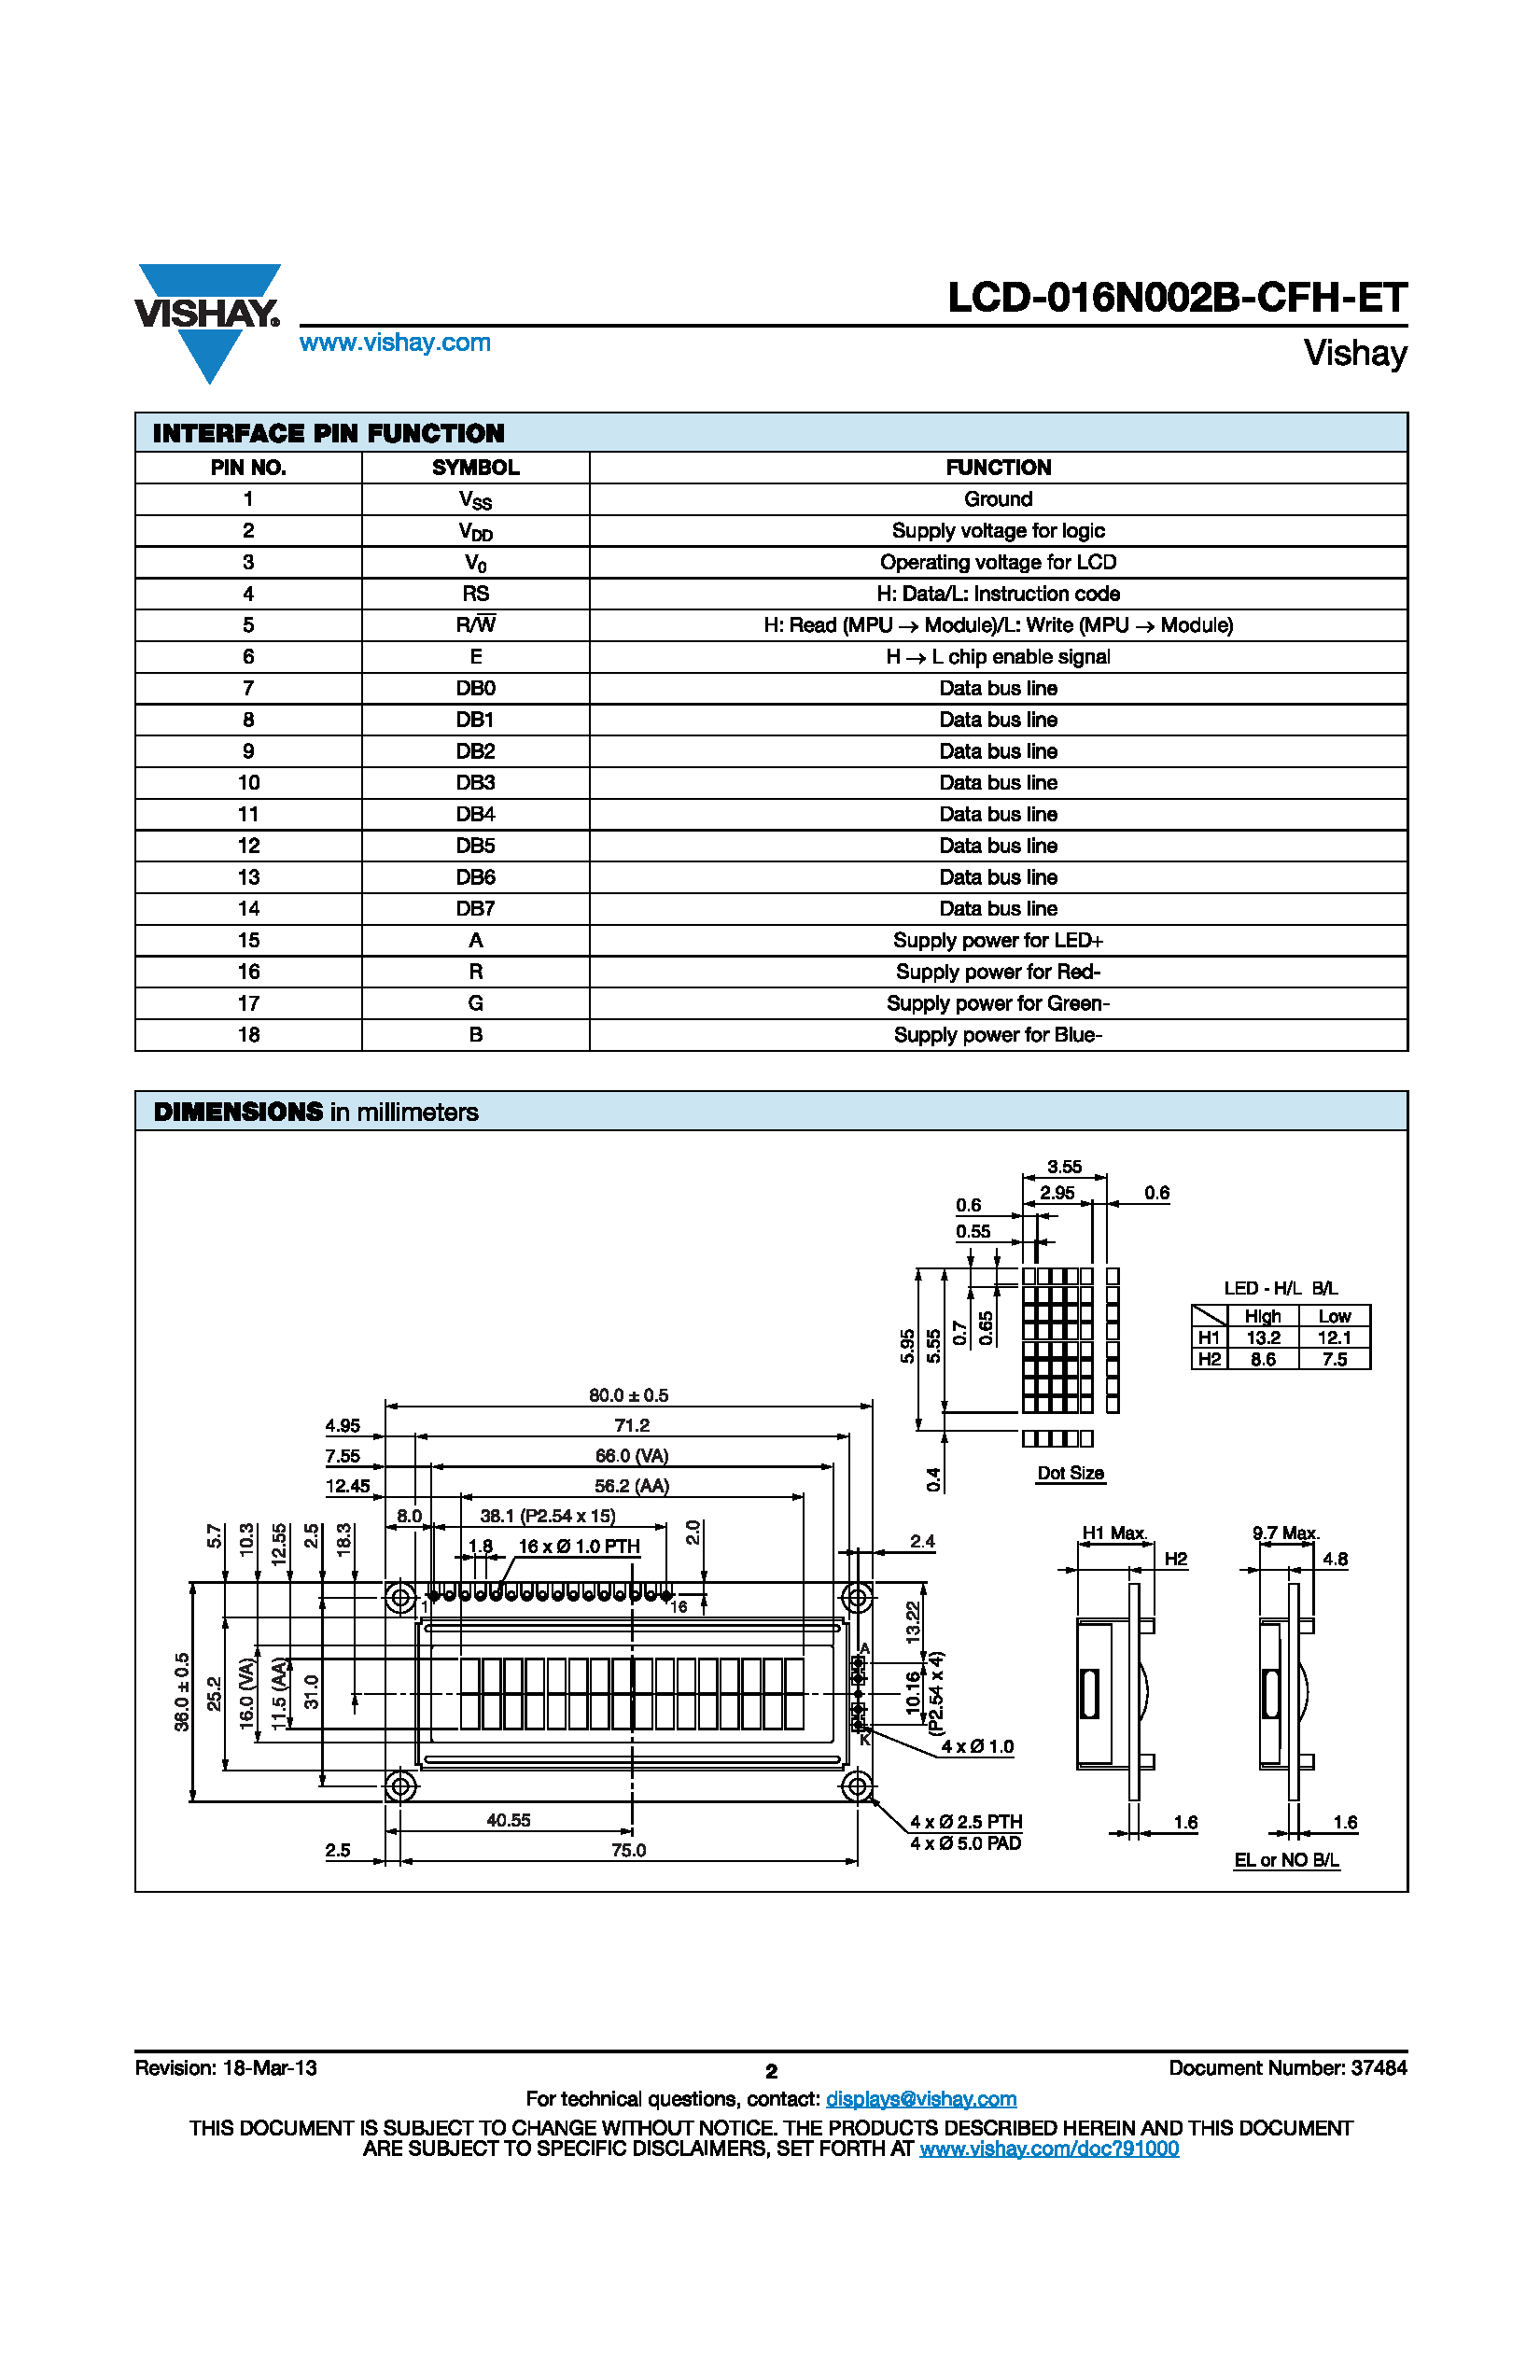
\includegraphics[trim = {30mm 65mm 90mm 250mm},clip,scale=0.5]{6/Img/lcd-16x2.pdf}
    %     \caption{Esquema LCD de 16x2}
    %     \label{fig:lcd-16x2}
    % \end{figure}
    % 
    % 
    % \begin{figure}[H]
    %     \centering
    %     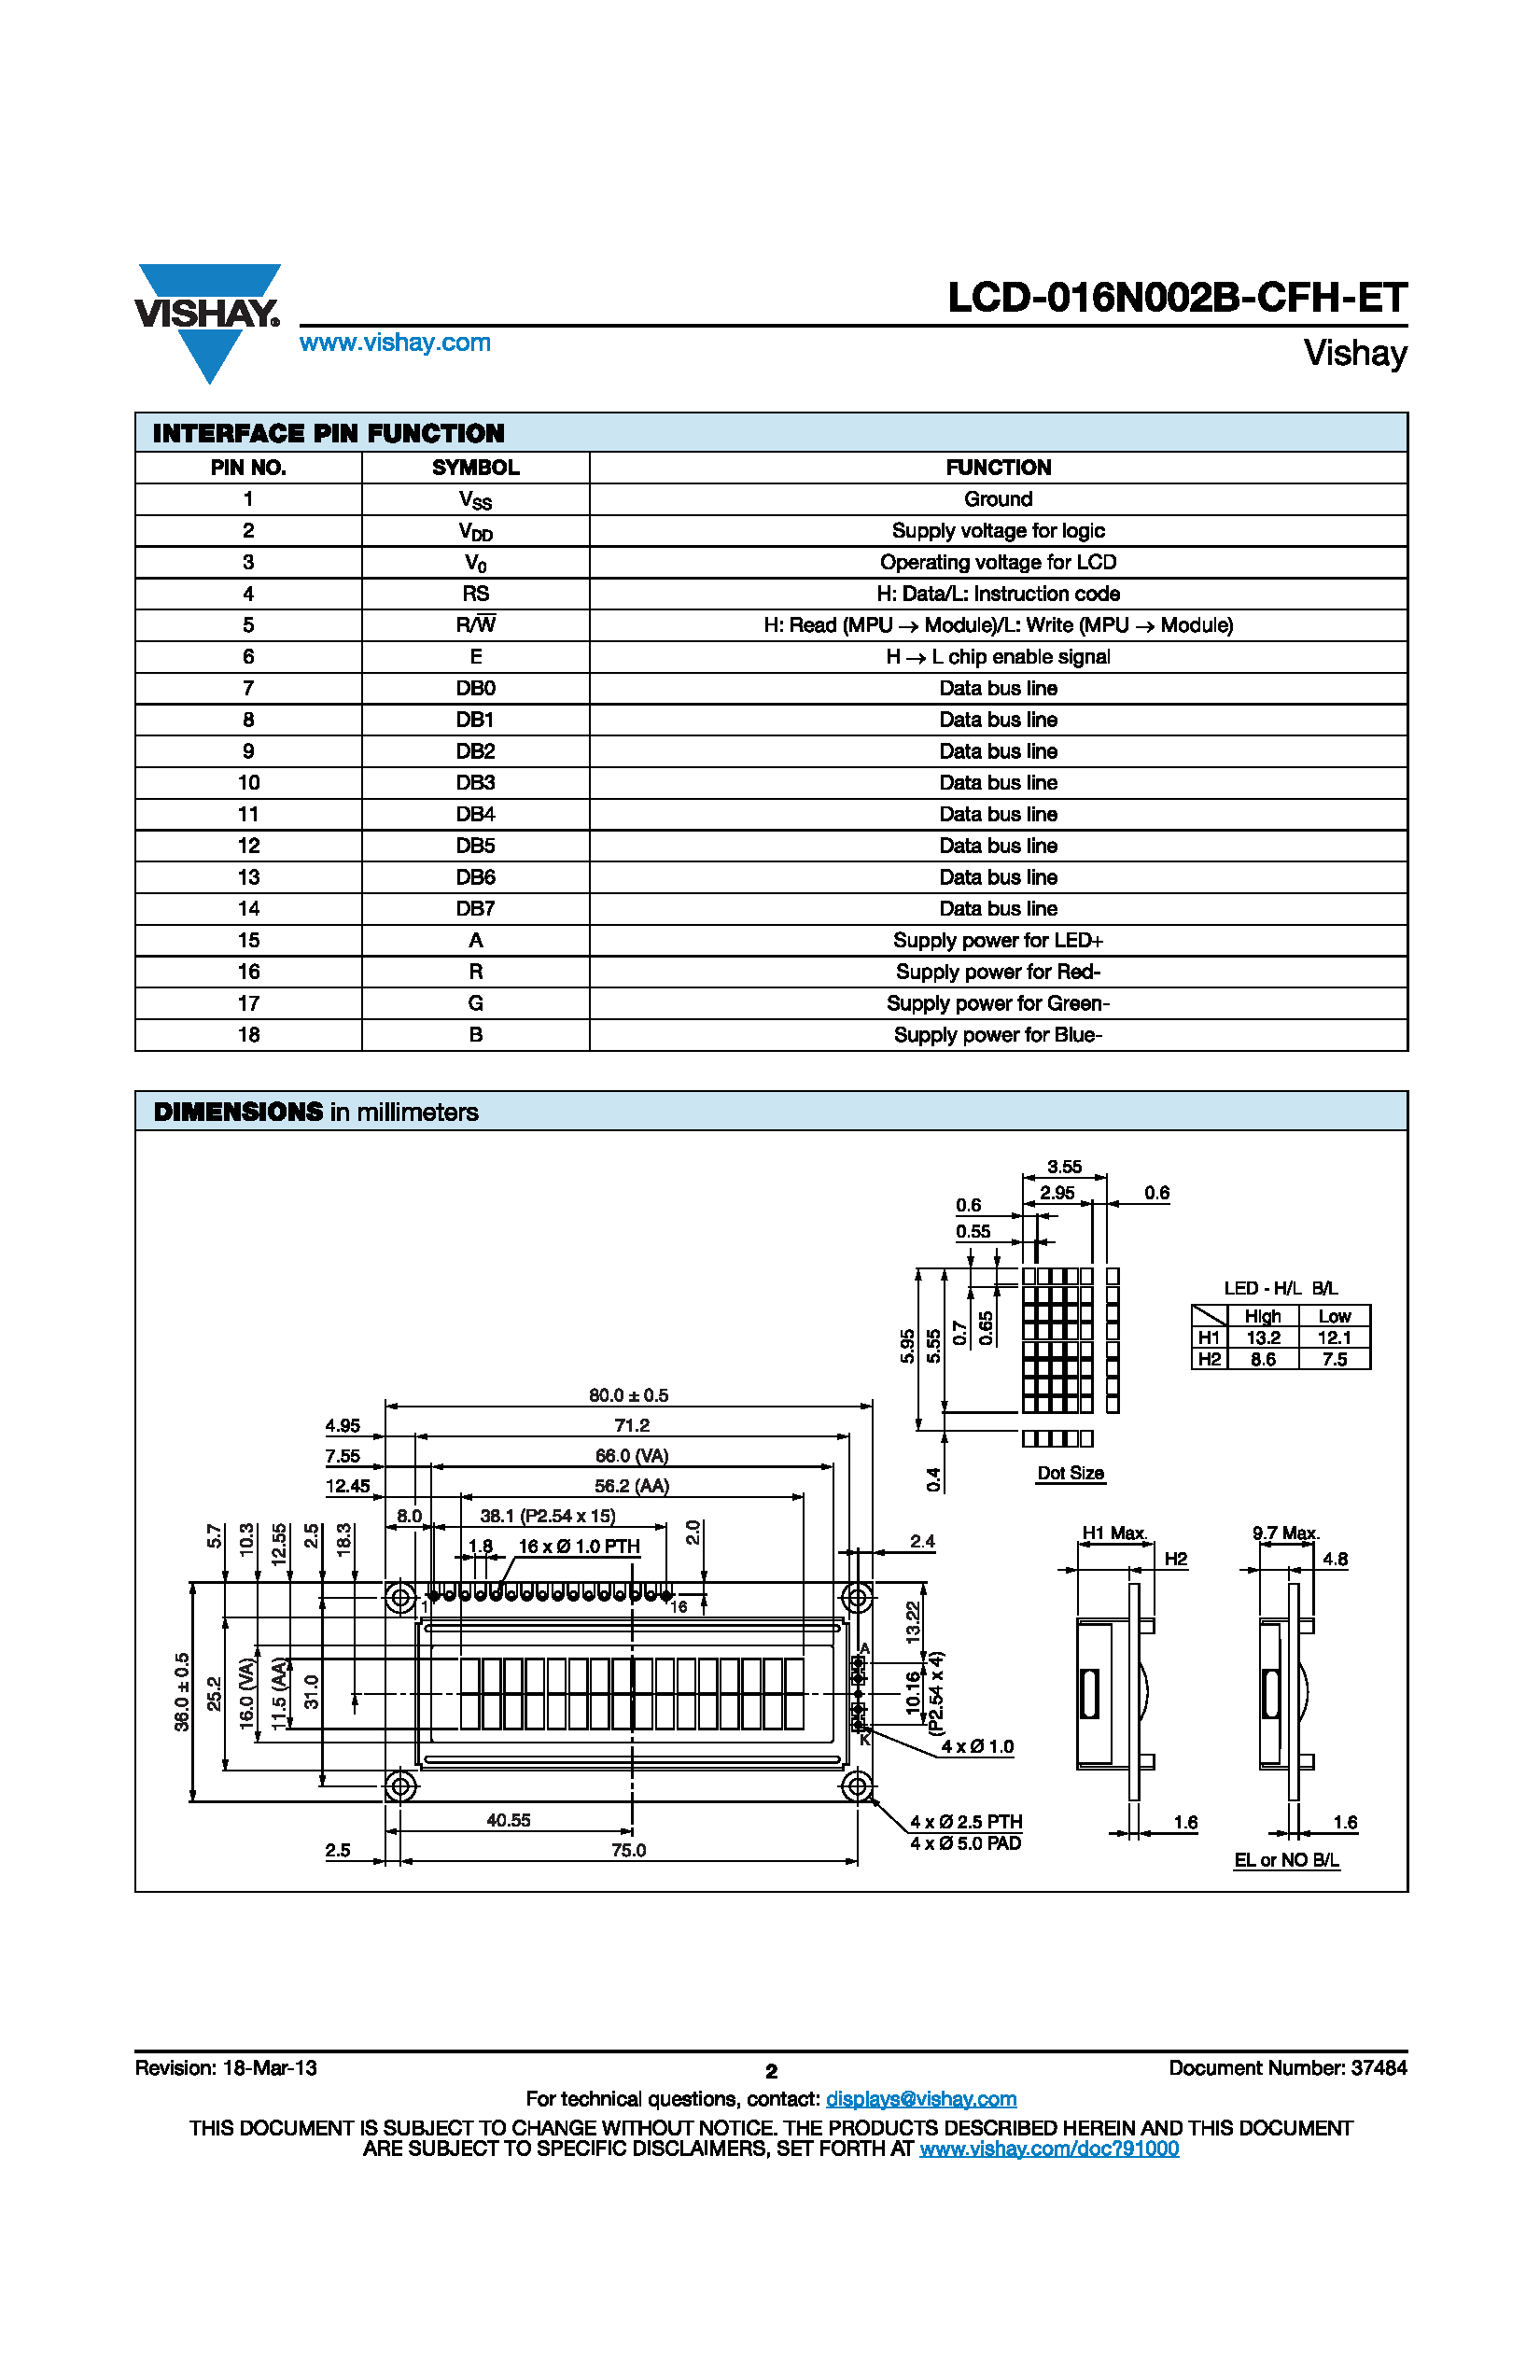
\includegraphics[trim = {30mm 250mm 90mm 20mm},clip,scale=0.5]{6/Img/lcd-16x2.pdf}
    %     \caption{Esquema LCD de 16x2}
    %     \label{fig:lcd}
    % \end{figure}
    % 
    % 
    % \subsection{Prepara tu documento}
    
    % Antes de que comiences a utilizar esta plantilla, es recomendable que prepare la información que contendrá en un archivo aparte. 
    % Ten preparadas tus gráficas, así como también las tablas aparte, para que sea más fácil integrarlo. 
    % Se recomienda fuertemente el uso de \textbf{formato Enhanced Metafile (.emf) para imágenes y gráficas} de resolución óptima. 
    % Finalmente, completa y organiza el contenido antes de darle el formato de esta plantilla. 
    % 
    % 
    \subsubsection{Identificación de capacidades}
    
    \begin{table}[H]
        \centering
        \caption{Recursos en materia de seguridad}
        \begin{tabular}{c c c}
        \hline
        \multicolumn{3}{c}{Inventario de recursos en materia de seguridad}\\
        \hline
             No.& Recurso & Cantidad  \\
        \hline
             1& Extintor & 2  \\
        \hline
             2& Botiquín & 3  \\
        \hline
             3& Detector de humo & 0 \\
        \hline
             4& Lampara de emergencia & 0 \\
        \hline     
        \end{tabular}
        \label{tab:inventario}
    \end{table}
    % 
    % 
    \subsubsection{Plano de localización de recursos}
    %
    %
    \begin{figure}[H]
        \centering
        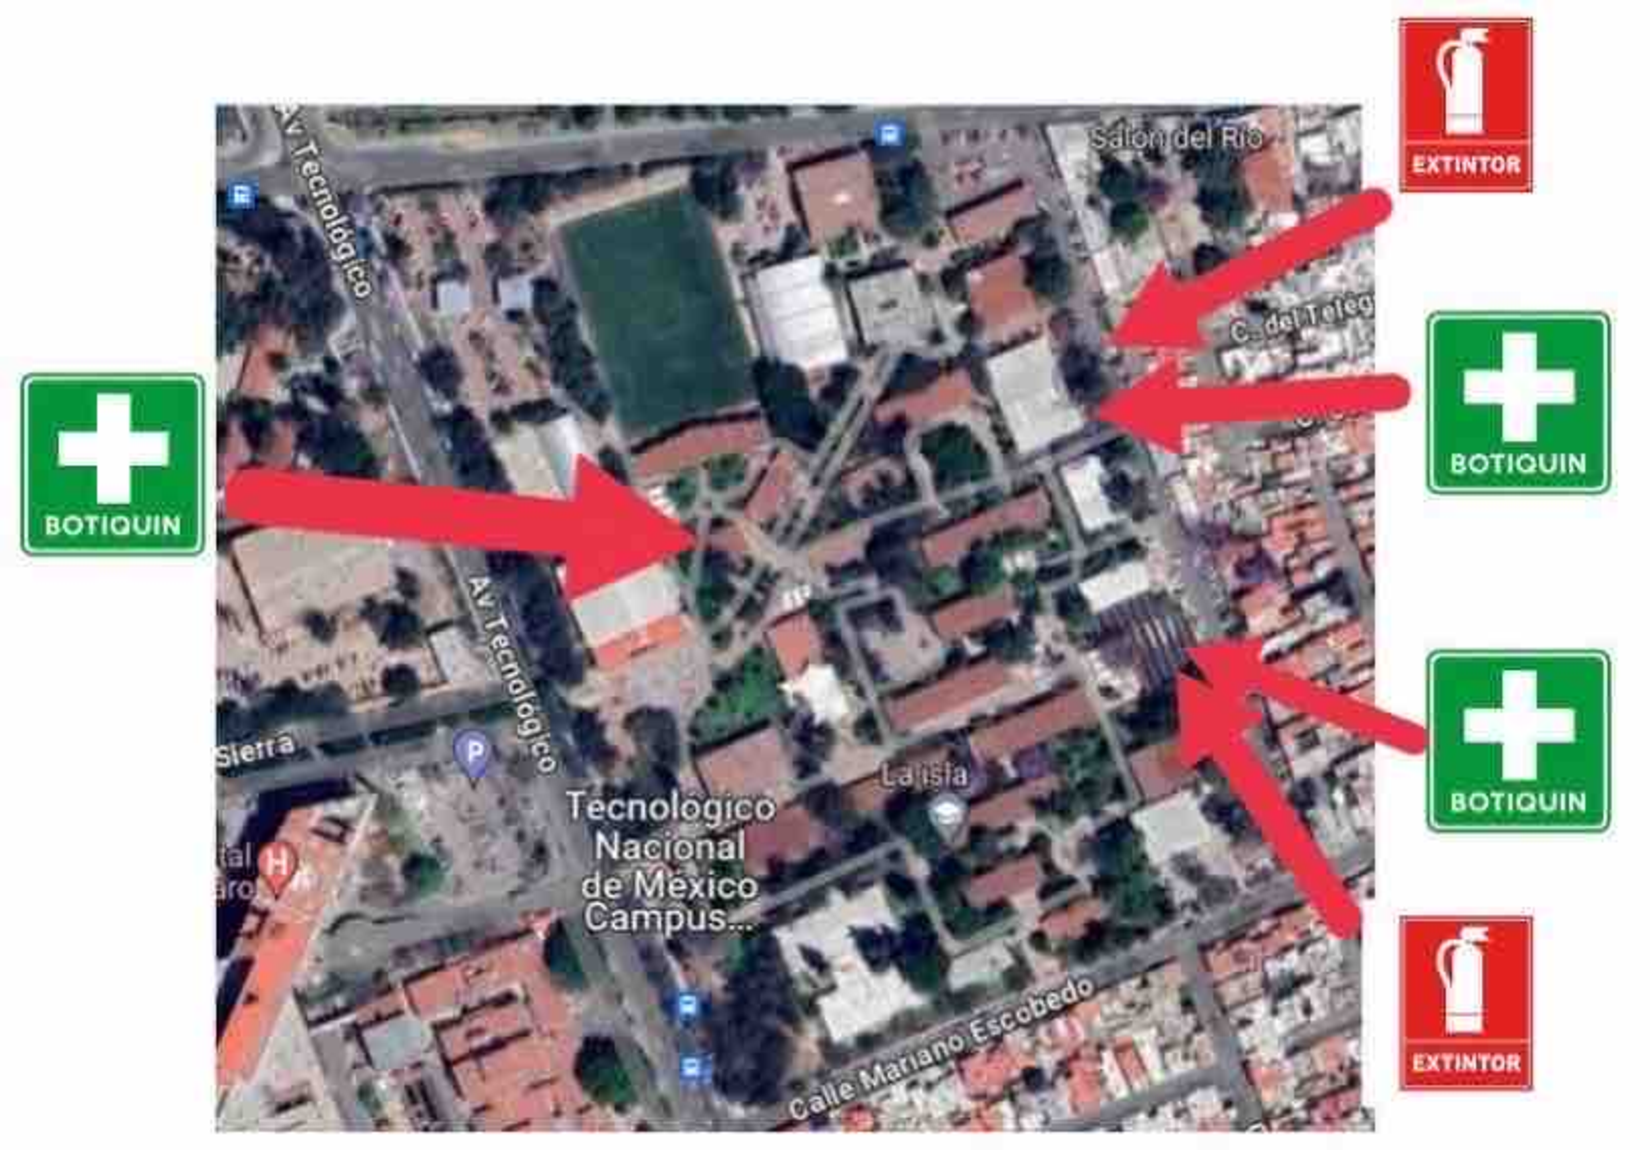
\includegraphics[trim = {1mm 1mm 1mm 1mm},clip,scale=0.3]{8/Img/Plano de los recursos en materia de seguridad.pdf}
        \caption{Plano del establecimiento de los recursos en materia de seguridad}
        \label{Plano de los recursos en materia de seguridad}
    \end{figure}
    % 
    %
    \subsubsection{ Identificación de apoyos externos}
    
    % 
    \begin{figure}[H]
        \centering
        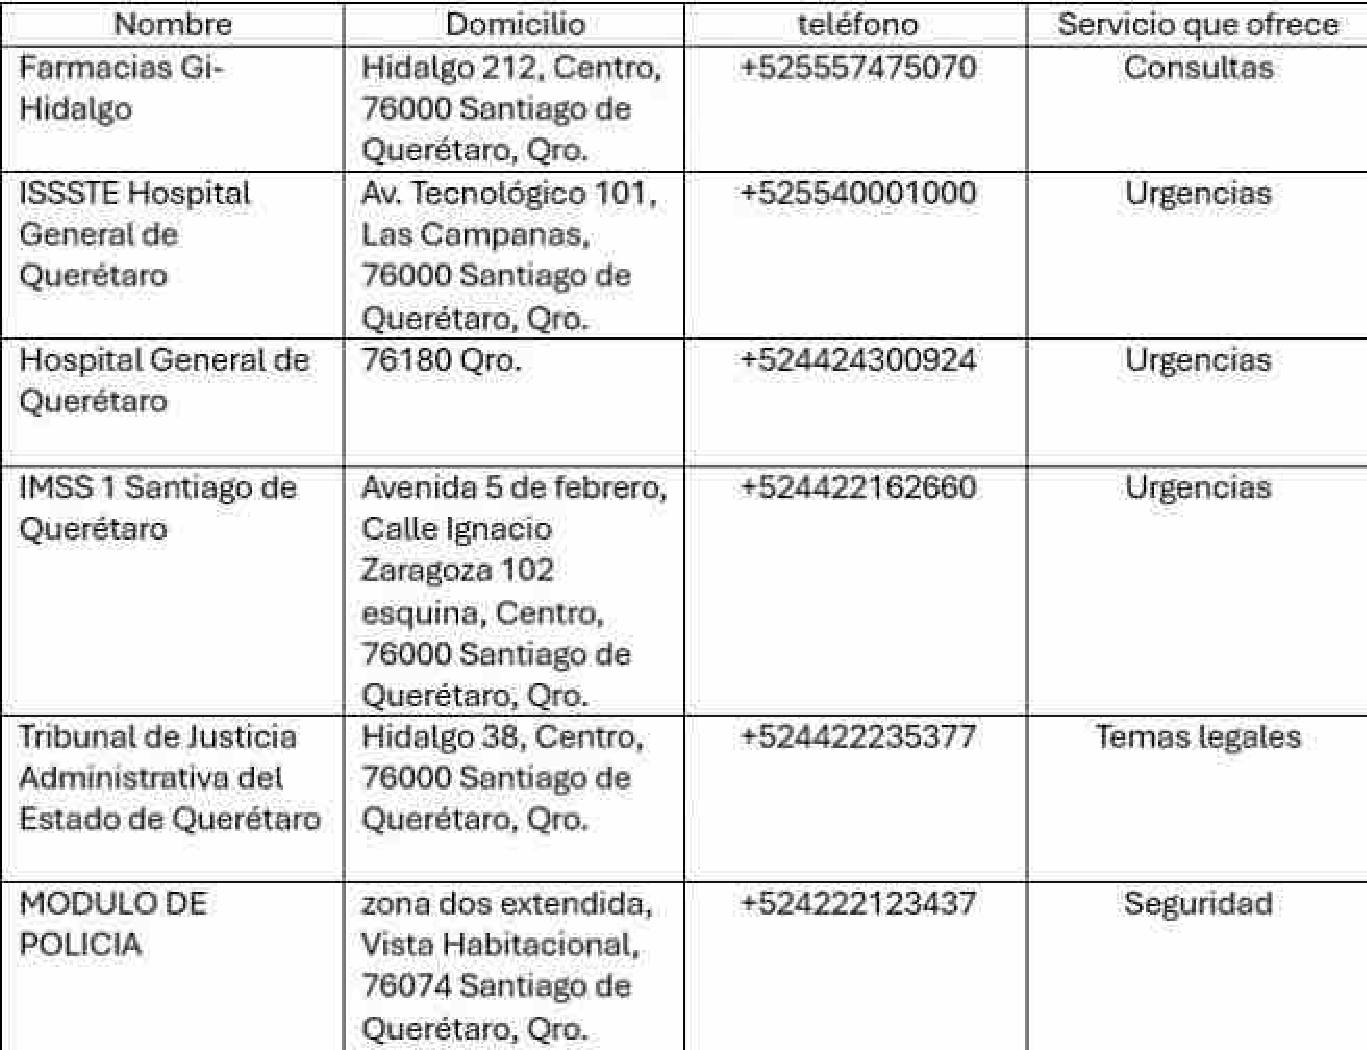
\includegraphics[trim = {1mm 1mm 1mm 1mm},clip,scale=0.3]{8/Img/Apoyos exteriores.pdf}
        \caption{ Lugares que servirán de apoyo en un situación de emergencia.}
        \label{Apoyos Exteriores}
    \end{figure}
    % 
    % }
    \subsubsection{Identificación de puntos de reunión}
    %
    \begin{figure}[H]
        \centering
        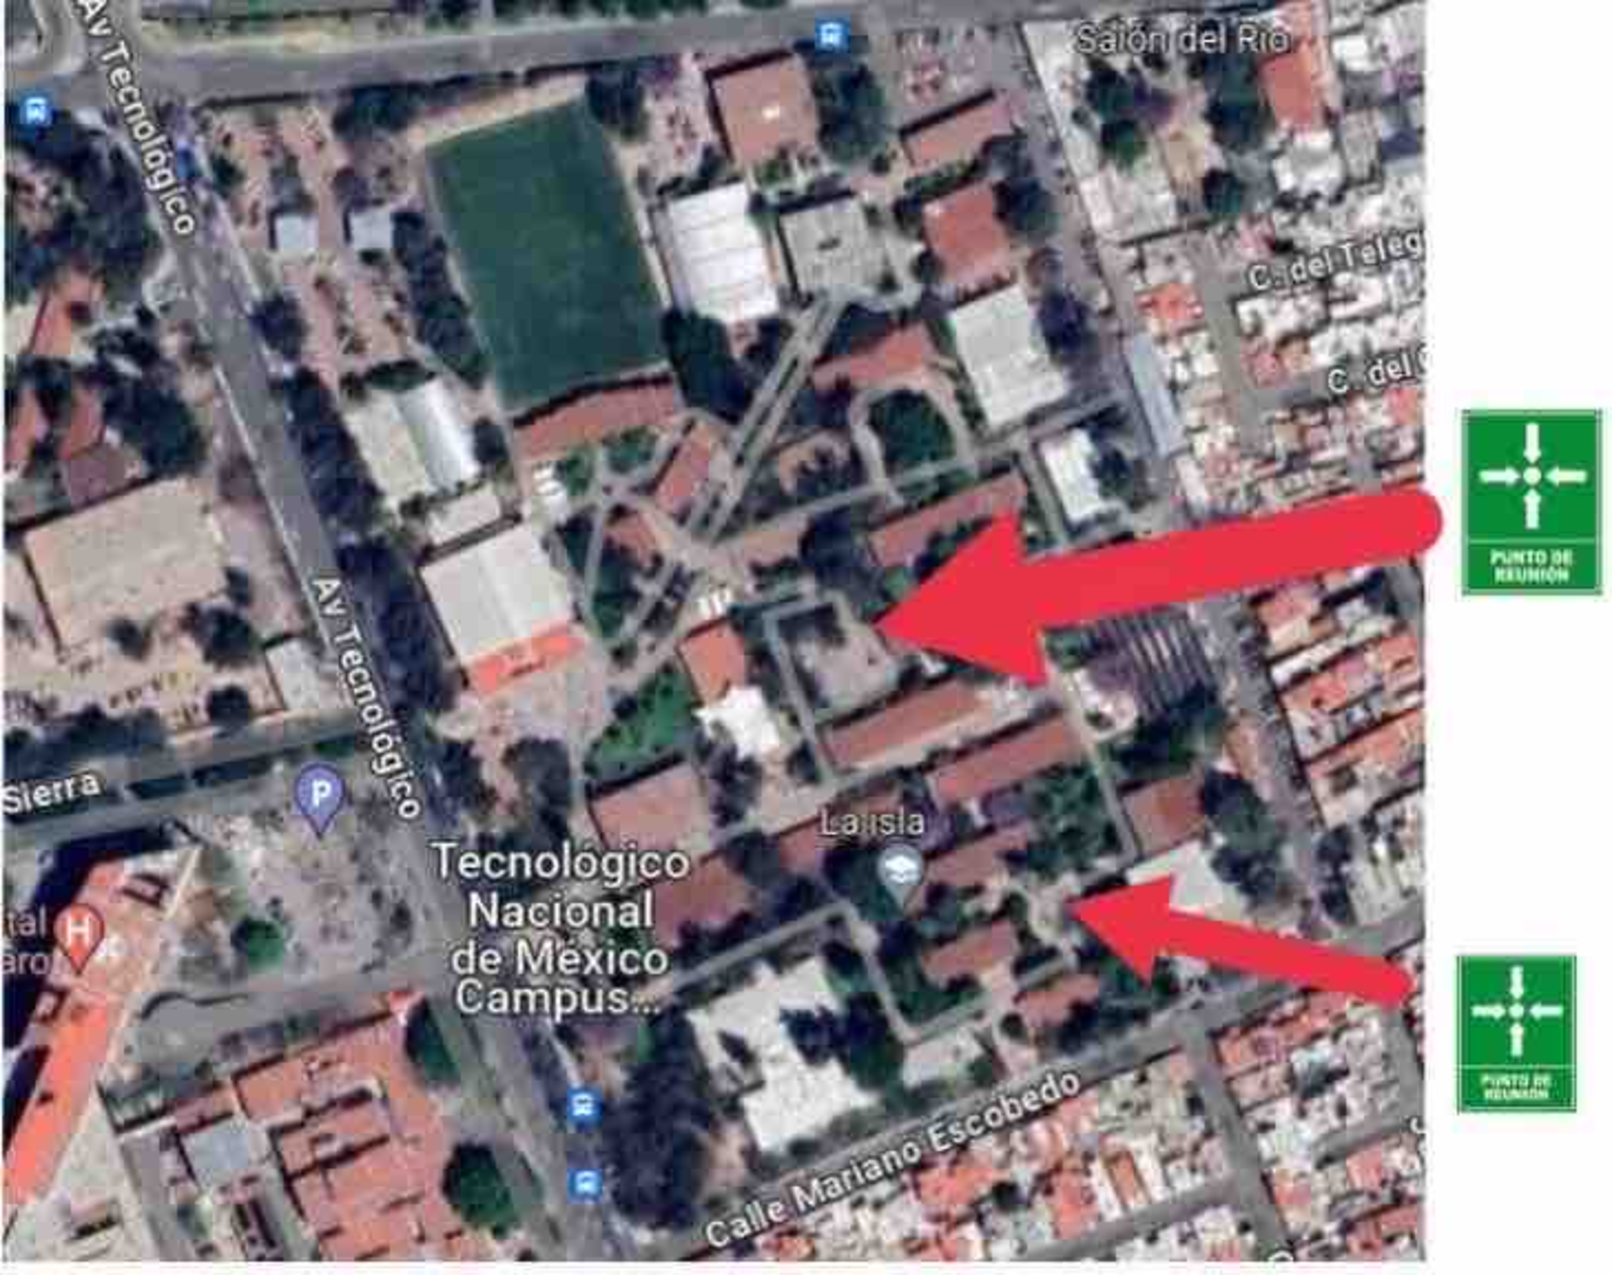
\includegraphics[trim = {1mm 1mm 1mm 1mm},clip,scale=0.3]{8/Img/Puntos de reunion.pdf}
        \caption{Zona segura en caso de una evacuación de emergencia.}
        \label{Puntos de reuinion}
    \end{figure}
    % 
    % 
    \subsubsection{Brigada de evacuación}
    
    % 
    % 
    \subsubsection{Directorio de telefónicos de emergencia}
    
    Listado telefónico de instituciones de atención de emergencias y otras instituciones que intervengan para el seguimiento y control de las mismas.
    
    \begin{figure}[H]
        \centering
        
\includegraphics[scale=0.5]{8/Img/911.pdf}
        \caption{Números de emergencia en posible riesgo}
        \label{Numeros de emergencia}
    \end{figure}
    % 
    % 
    \begin{figure}[H]
        \centering
        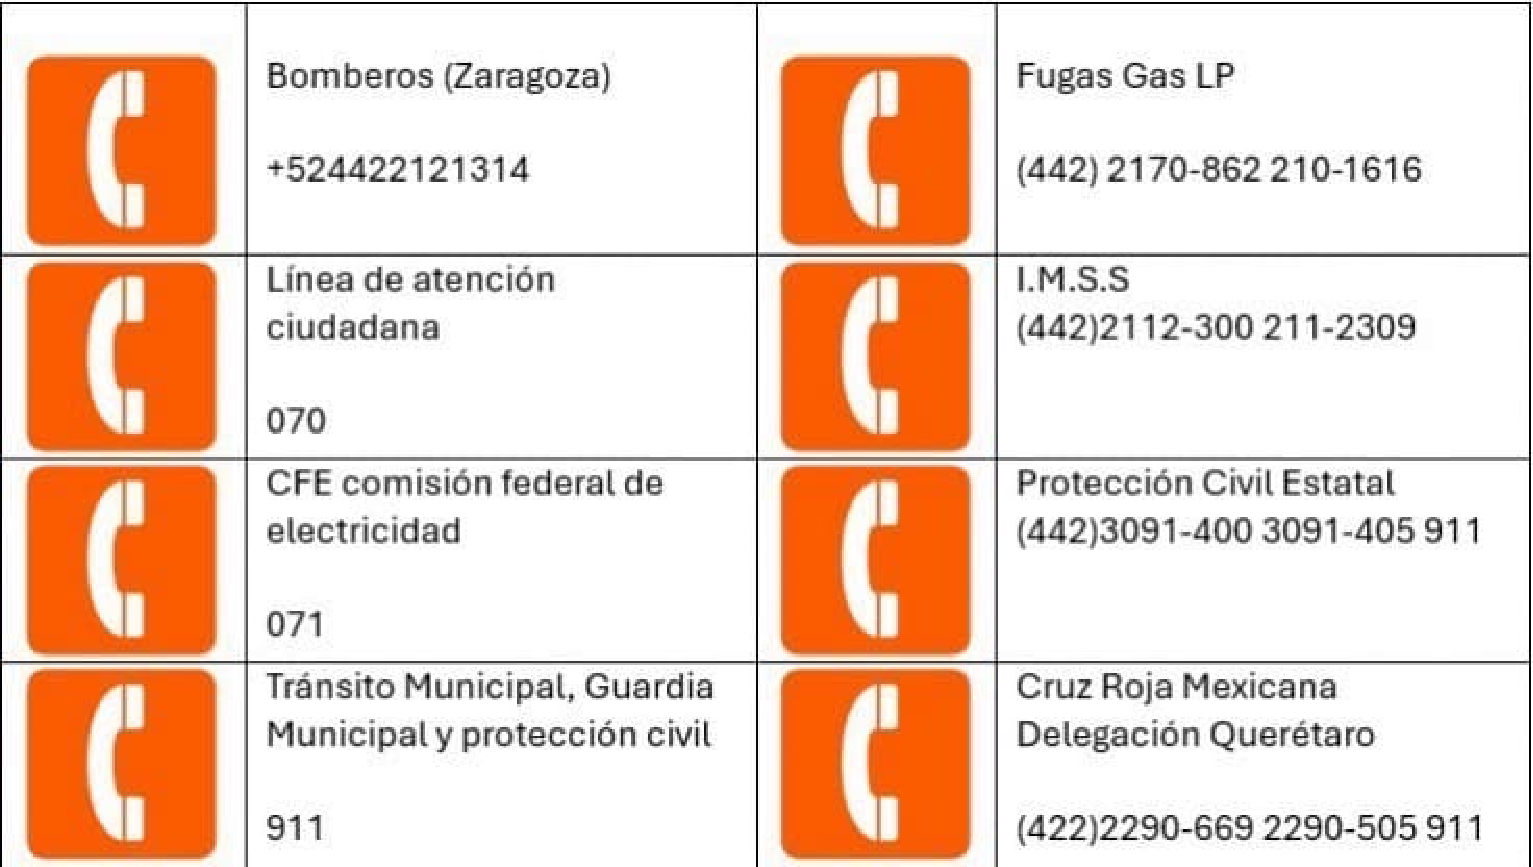
\includegraphics[scale=0.3]{8/Img/Directorio.pdf}
        \caption{Números de emergencia de emergencia más próximos a la ubicación el posible riesgo}
        \label{Directorio}
    \end{figure}
    % 
    % 
    \subsection{Análisis de los métodos, materiales, herramientas e instalación utilizada en la ejecución del ensamble de un circuito electrónico}
    
    \subsubsection{Verificación}
    A partir de la planificación se tomo de referencia para llevar a cabo un orden de la realización del ensamble a partir de etapas, sin embargo nada salio como lo planeado, el primer paso que era la realización de una guía para que el operario pudiera realizar el ensamble,este paso se cumplió, la obtención de los materiales seria el segundo aunque al inicio se tenia planteado que nosotros no gastáramos y solo tomáramos prestado los materiales del profesor eso tuvo que cambiar después que un par de compañeros terminaran dañando 2 diferentes ESP32 lo cual provoco que nos retrasáramos de gran manera debido a que tuvimos que esperar a que llegaran y alguno tuvimos que cambiar nuestros manuales.
    % 
    % 
    \subsubsection{Desarrollo del sistema de tiempos predeterminado}
    Véase tabla \ref{Diagrama Bimanual}
    % 
    %  
    \subsubsection{Desarrollo del muestreo del trabajo}
    % 
    % 
    \subsubsection{Corrección por balanceo de procesos}
    % 
    % 
    \subsubsection{Datos estándar continuos y discretos}
    % 
    % 
    \subsection{Diseño de la forma más económica de realizar el trabajo}
    Después de hacer el ensamble y hacer el análisis de los tiempos estándar y tiempos ciclos se hizo un análisis para llevar a cabo una normalización de los materiales con el fin de encontrar la forma mas económica de hacer el trabajo, para el análisis se cuenta con la siguiente tabla \ref{Diseño para hacer mas economico el trabajo}
    Con esta tabla podemos comparar la diferencia de precios, de primera impresión puede parecer que la suma de los materiales para el nuevo ensamble puede ser mayor al viejo ensamble, sin embargo lo que buscamos es anticiparnos a los contratiempos que podemos encontrar los cuales si no tenemos previstos con anticipación pueden resultar mas costosos y generar mas gastos ante la urgencia de querer terminar el ensamble pues compraremos materiales disponibles en vez de comprar los materiales necesarios.
    
    % 
    % 
    \subsection{Normalización de los métodos, materiales, herramientas e instalaciones}
    
    % 
    % 
    \subsection{Determinación del tiempo estándar para que una persona competente realice el trabajo con marcha normal}
    Véase tabla \ref{Tabla de unidades TMU}
    % 
    % 
    0Antes de que comiences a utilizar esta plantilla, es recomendable que prepare la información que contendrá en un archivo aparte. 
    Ten preparadas tus gráficas, así como también las tablas aparte, para que sea más fácil integrarlo. 
    Se recomienda fuertemente el uso de \textbf{formato Enhanced Metafile (.emf) para imágenes y gráficas} de resolución óptima. 
    Finalmente, completa y organiza el contenido antes de darle el formato de esta plantilla. 
    
    \subsection{Acrónimos y Abreviaciones}
    
    Los acrónimos y abreviaciones deberán ser definidos únicamente la primera vez que aparecen en el texto, esto para que el lector entienda lo que significan.
    
    \subsection{Ecuaciones}
    
    %Las ecuaciones son una excepción a las especificaciones prescritas de esta plantilla. 
    %Deberá determinar si su ecuación debe escribirse o no utilizando la f%uente Adobe Devangari. 
    %Para crear ecuaciones multinivel, puede ser necesario tratar la ecuación como un gráfico e insertarla en el texto después de aplicar el estilo de la platilla.
    %Las ecuaciones serán enumeradas de manera consecutiva, y el número de ecuación, entre paréntesis, se colocan al ras de la derecha, utilizando una tabulación derecha. 
    
    %\begin{equation}
       % \label{eq1}
       % x + y = z 
    %\end{equation}
    
    %Es importante asegurarse de que los símbolos de la ecuación sean definidos antes o inmediatamente después de la ecuación. Utilice “(1)”, en vez de “Eq. 1” al enumerar las ecuaciones, excepto al principio de una oración: “La ecuación (\ref{eq1}) es…”
    
    \subsection{Distribución uniforme discreta}
    La media de la variable aleatoria discreta (X) es:
    \begin{equation}
         \mu_x=\dfrac{b+a}{2}
    \end{equation}
    
    La desviación estándar de X es:
    \begin{equation}
         \sigma_x=\sqrt{\dfrac{(b-a+1)^2-1}{12}}
    \end{equation}
    
    
    \section{Resultados y discusión}
    
    \begin{figure}[H]
        \centering
        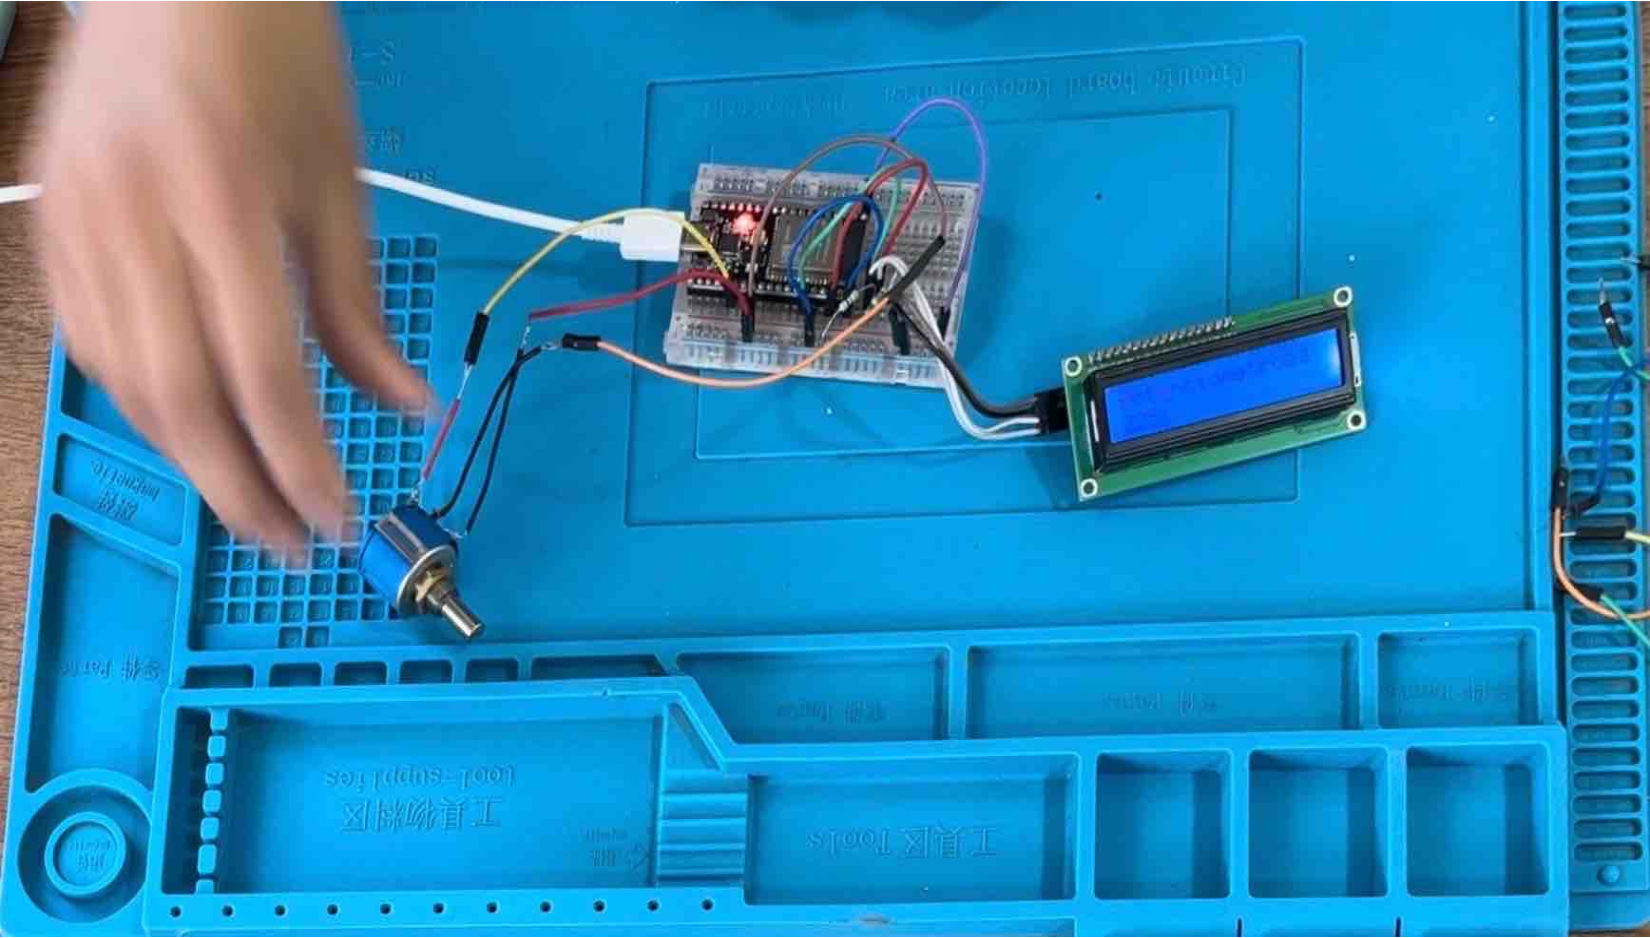
\includegraphics[trim = {0mm 0mm 0mm 0mm},clip,scale=0.2]{8/Img/Evidencia 1.pdf}
        \caption{Evidencia 1}
        \label{Evidencia 1}
    \end{figure}
    
    \begin{figure}[H]
        \centering
        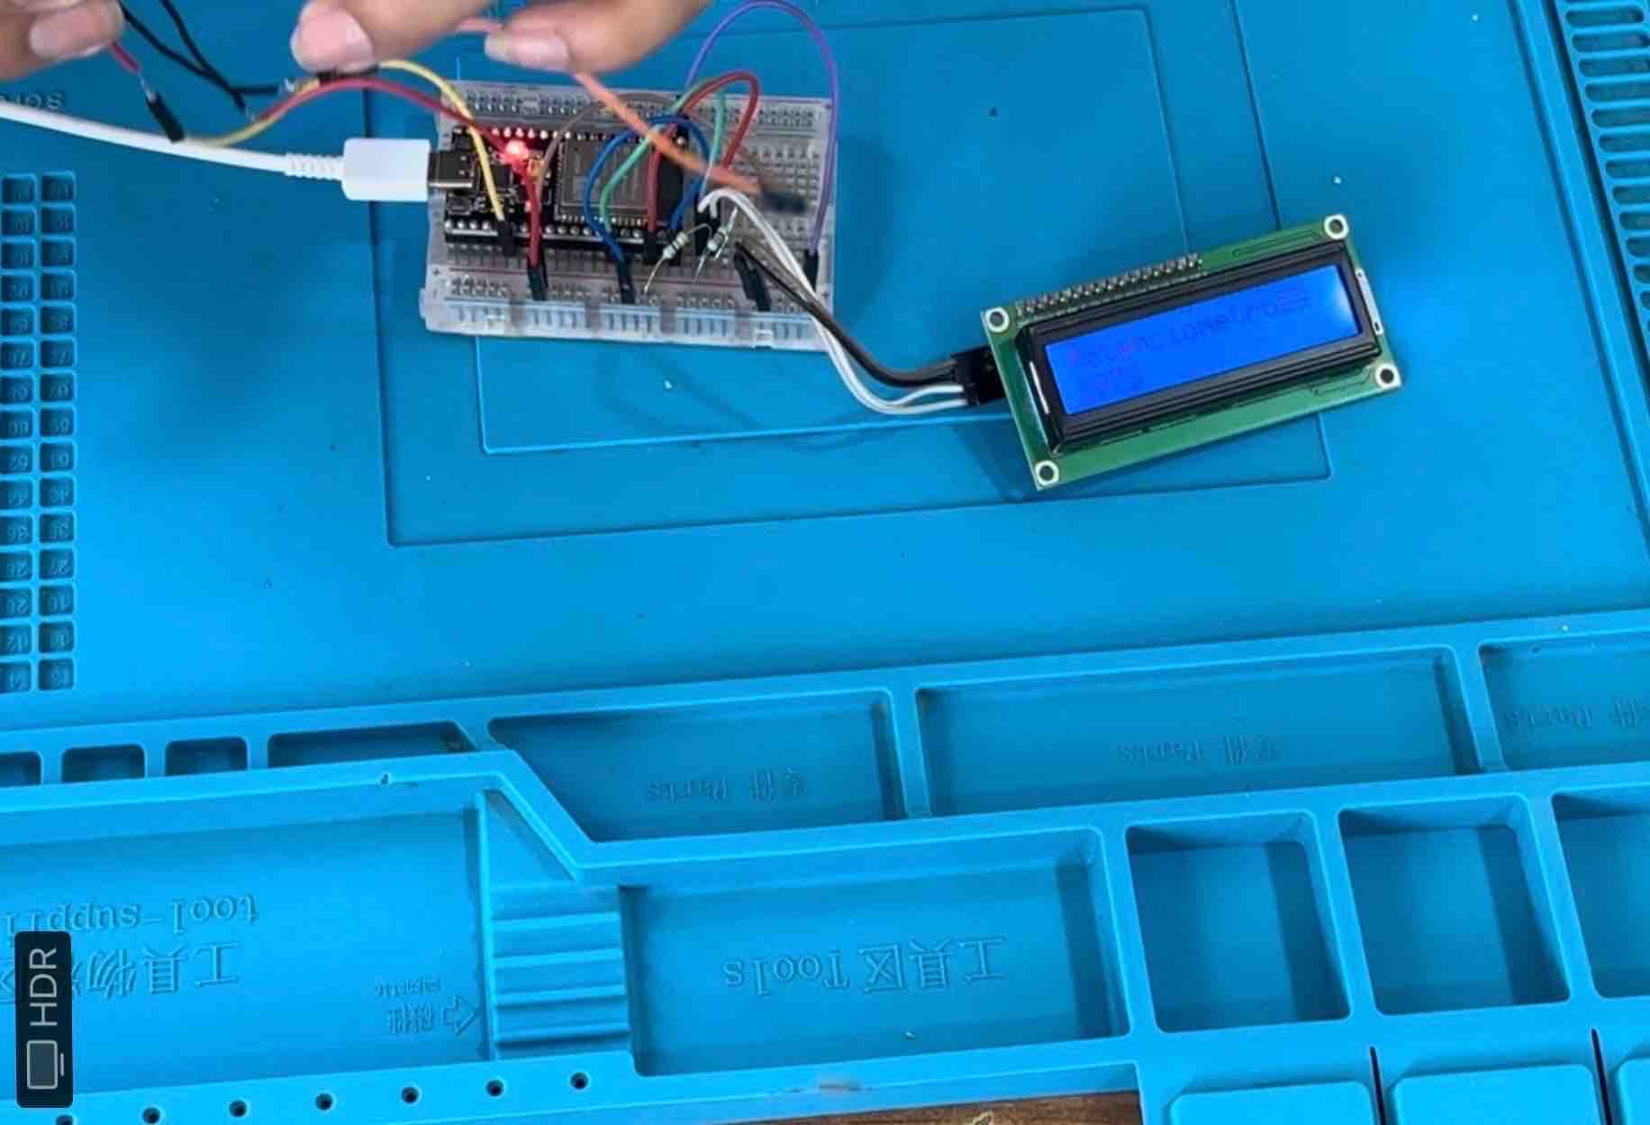
\includegraphics[trim = {0mm 0mm 0mm 0mm},clip,scale=0.2]{8/Img/Evidencia 2.pdf}
        \caption{Evidencia 2}
        \label{Evidencia 2}
    \end{figure}
    
    \begin{figure}[H]
        \centering
        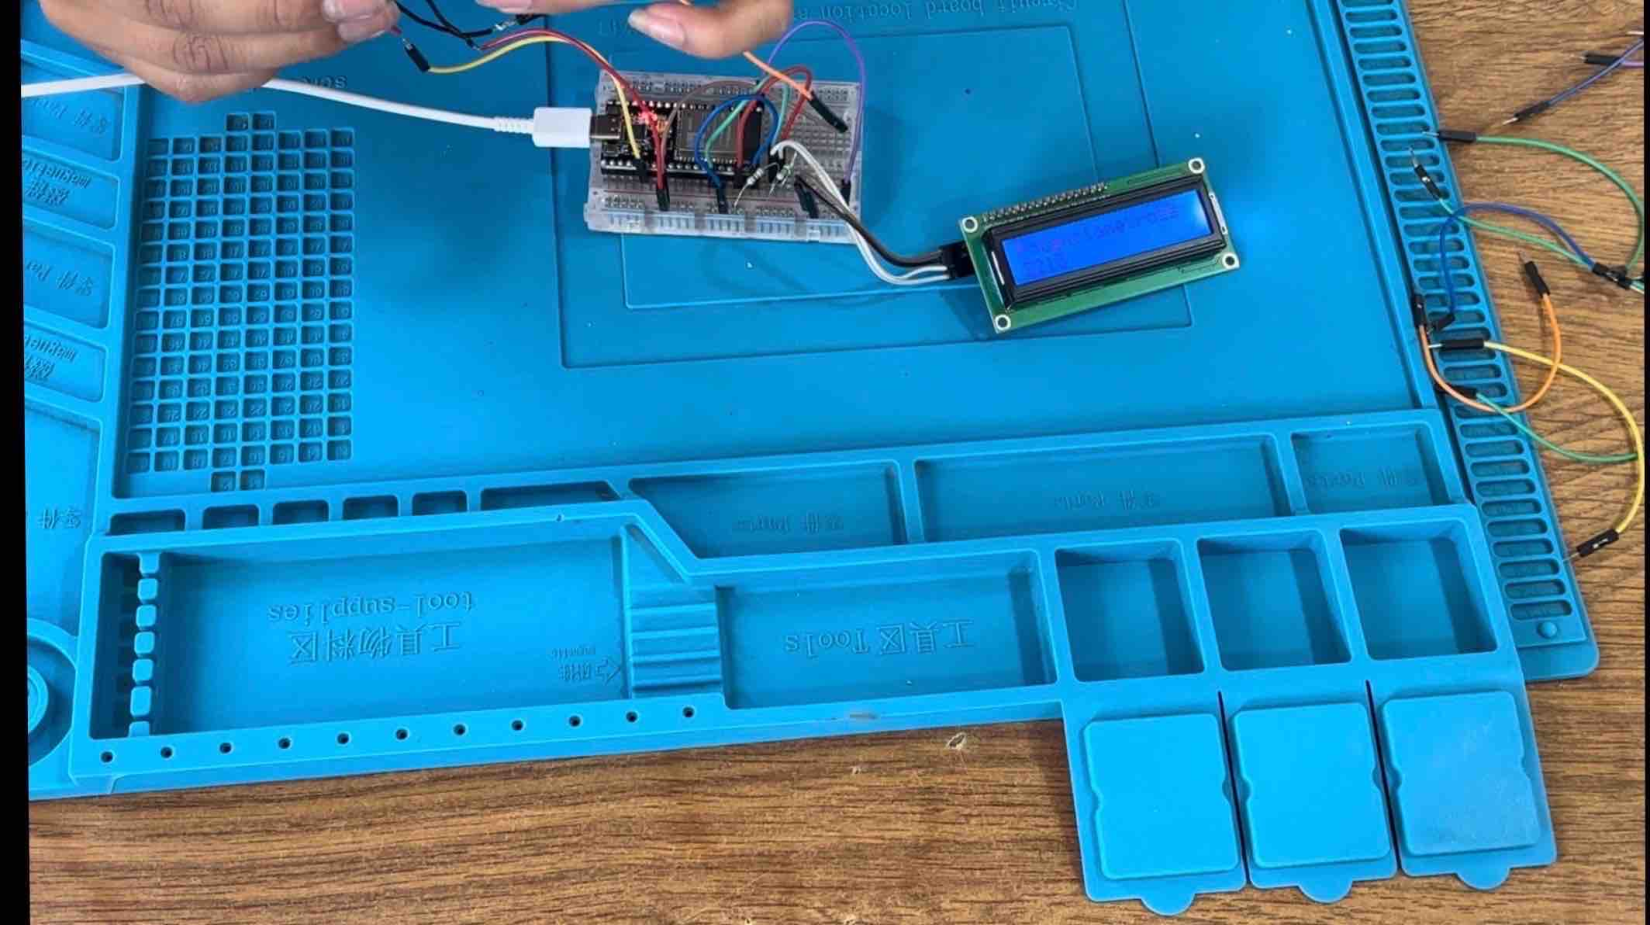
\includegraphics[trim = {0mm 0mm 0mm 0mm},clip,scale=0.2]{8/Img/Evidencia 3.pdf}
        \caption{Evidencia 3}
        \label{Evidencia 3}
    \end{figure}
    
    \begin{figure}[H]
        \centering
        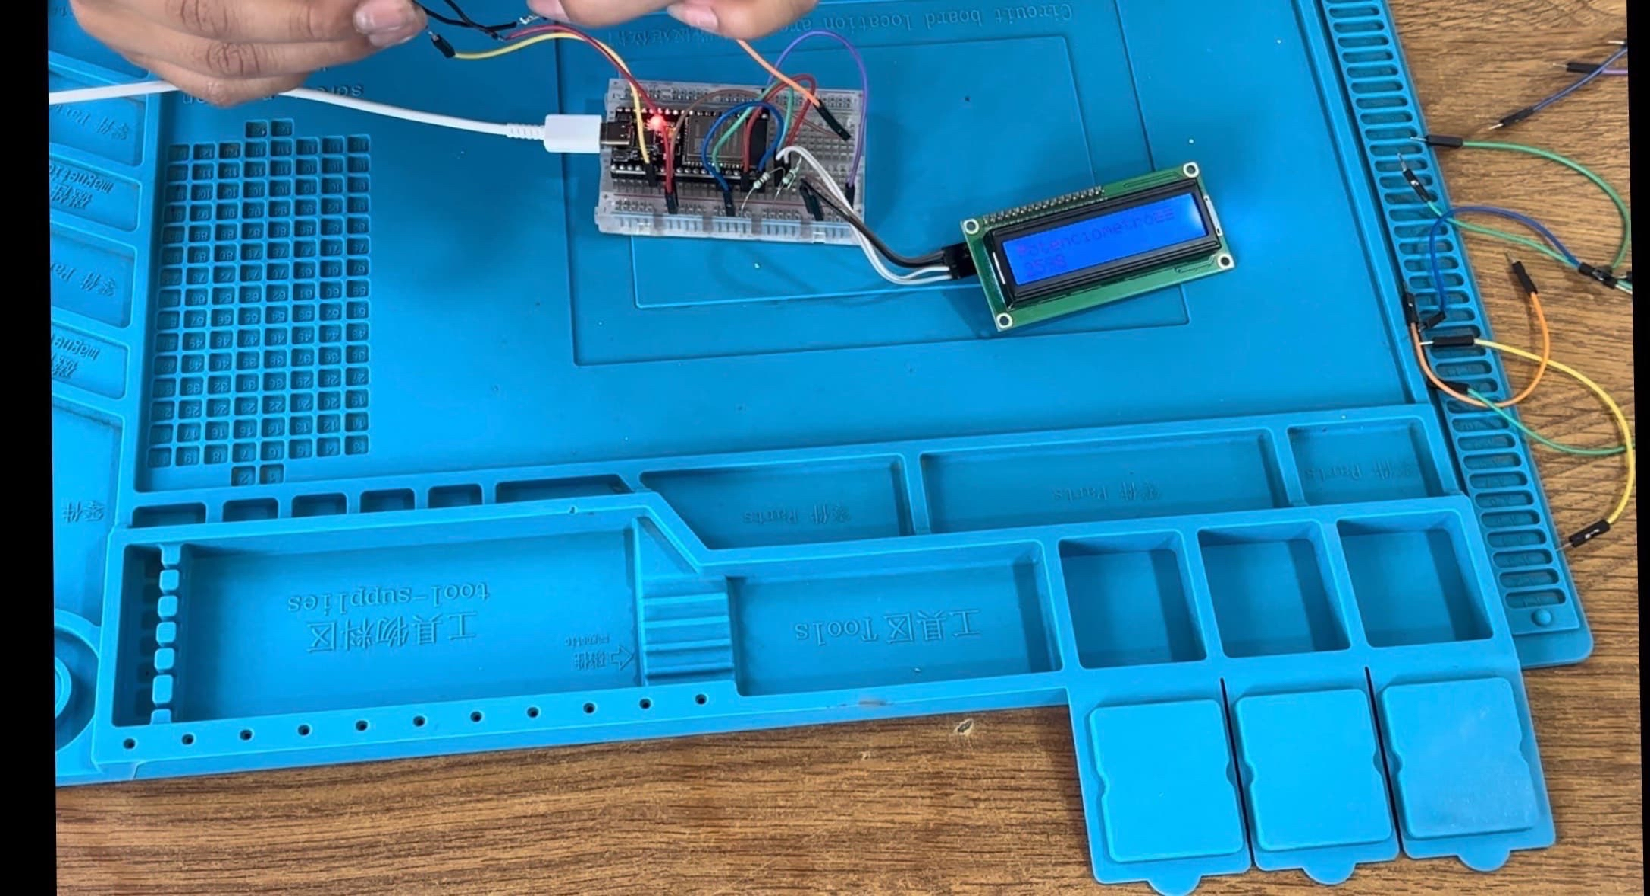
\includegraphics[trim = {0mm 0mm 0mm 0mm},clip,scale=0.2]{8/Img/Evidencia 4.pdf}
        \caption{Evidencia 4}
        \label{Evidencia 4}
    \end{figure}
    
    
    
    %Antes de comenzar a preparar tu artículo, es importante que lea primero la guía del autor, la cual incluye los temas o apartados que son necesarios para tener tu trabajo completo.
    %Una vez completada la edición del texto, el documento está listo para el uso de esta plantilla. En este archivo recién creado, resalte todo el contenido e importe el archivo de texto preparado. Ahora esta listo para estilizar su documento.
    %En esta sección se deben presentar todo lo obtenido de la sección 2, incluidas deducciones o efectos del desarrollo. También se podrán incluir subsecciones numeradas de la siguiente forma:
    \begin{figure}[H]
        \centering
        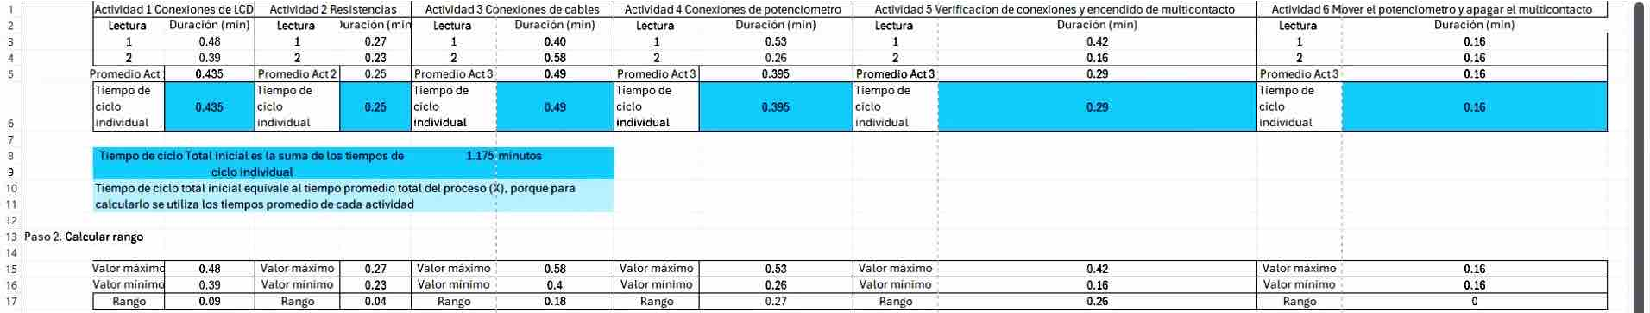
\includegraphics[trim = {0mm 0mm 0mm 0mm},clip,scale=0.3]{8/Img/Tiempos estandar.pdf}
        \caption{Tabla de tiempos estándar}
        \label{Tiempos estándar}
    \end{figure}
    
    Después de realizar las 2 muestras tomando vídeo del operario podemos obtener la tabla de tiempos estándar dividiendo la operación en actividades para poder llevar acabo la obtención de los tiempos estándar y en base a esto poder estandarizar la operación para hacer mas eficiente el trabajo, esto va de la mano del estudio de movimientos y tiempos ya que al ver los tiempos podemos hacer un análisis para eliminar los movimientos que creemos innecesarios y posteriormente mejorar los tiempos de la operación lo cual nos ayudara disminuir costos 
    
    
    
    \section{Conclusiones}
    
    Se describe aquí el alcance del trabajo, logros obtenidos y perspectivas para el futuro de este. Se sugiere colocar información cuantitativa obtenida.
    
    \section{Agradecimientos}
    
    Es importante darles su debido reconocimiento a los laboratorios, instituciones, organizaciones, entre otros que han sido participes para la culminación de este trabajo. También es importante mencionar, fondos, proyectos, becas, entre otros que se le han otorgado al o los autores para realizar el trabajo de investigación. Ejemplo: “Los autores agradecen al Concejo Nacional de Ciencia y Tecnología por los recursos otorgados…”
    
    \section*{Referencias}
    Para esta platilla, se solicita al autor enumerar las citas de manera consecutiva entre corchetes 
    La puntuación de la oración que sigues sería  
    Refiérase simplemente al número de referencia, como en , no utilice “Ref. [3]” o “referencia [3]” excepto al principio de una oración: “La referencia [3] fue la primera…”
    Enumere las notas al pie por separado en superíndices. Coloque la nota de pie de en la parte inferior de la columna en la que se citó. No coloque notas al pie en la lista de referencias. Utilice letras para las notas al pie de la tabla.
    A menos de que haya tres autores o más; no utilice “et al.”. Los trabajos que no hayan sido publicados, incluso si han sido presentados para su publicación, deben ser citados como “inéditos”. Los trabajos que han sido aceptados para su publicación deben de citarse como “en prensa”. Poner en mayúscula sólo la primera palabra de un título, excepto los nombres propios y los símbolos de elemento. 
    Otros ejemplos 
    Véase el archivo adjunto 
    
    % Ejemplo
    %  @Article{article,
    % 	author = "Author1 LastName1 and Author2 LastName2 and Author3 LastName3",
    % 	title = "Article Title",
    % 	volume = "30",
    % 	number = "30",
    % 	pages = "10127-10134",
    % 	year = "2013",
    % 	doi = "10.3389/fnins.2013.12345",
    % 	URL = "http://www.frontiersin.org/Journal/10.3389/fnins.2013.12345/abstract",
    % 	journal = "Frontiers in Neuroscience"
    % }
    
    % @book{book,
    %   author    = {Author Name}, 
    %   title     = {The title of the work},
    %   publisher = {The name of the publisher},
    %   address   = {The city},
    %   year      = 1993,
    % }
    
    % @incollection{chapter,
    %   author       = {Bauthor Surname}, 
    %   title        = {The title of the work},
    %   editor       = {Editor Name},
    %   booktitle    = {The title of the book},
    %   publisher    = {The name of the publisher},
    %   address      = {The city},
    %   year         = 2002,
    %   pages        = {201-213},
    % }
    
    % @InProceedings{conference,
    %   author = {Cauthor Name and Dauthor Surname and Fauthor LastName},
    %   title = {The title of the work},
    %   booktitle = {The title of the conference proceedings},
    %   year = 1996,
    %   publisher = {The name of the publisher},
    %   editor = {Editor Name1 and Editor Name2},
    %   pages = {41-50},
    % }
    
    % @book{cho,
    %   author       = {Gauthor Name1}, 
    %   title        = {The title of the work},
    %   publisher = {Country code and patent number},
    %   address      = {Patent Country},
    %   year = 2013
    % }
    
    % @book{patent,
    %   author    = {Hauthor Surname1}, 
    %   title     = {The title of the work},
    %   publisher = {Patent number},
    %   address   = {Patent country},
    %   year      = 2010,
    % }
    
    % % please use misc for datasets
    % @misc{dataset, 
    % 	author = "Author1 LastName1 and Author2 LastName2 and Author3 LastName3",
    % 	title = "Data Title",
    % 	year = "2011",
    % 	doi = "10.000/55555",
    % 	URL = "http://www.frontiersin.org/",
    % }
    
    % 
    % 
    %%%%%%%%%%%%%%%%%%%%%%%%%%%%%%%%%%
    \appendix
    %%%%%%%%%%%%%%%%%%%%%%%%%%%%%%%%%%
    % 
    % 
    \centering{\section[\appendixautorefname{}]{APÉNDICE}}
    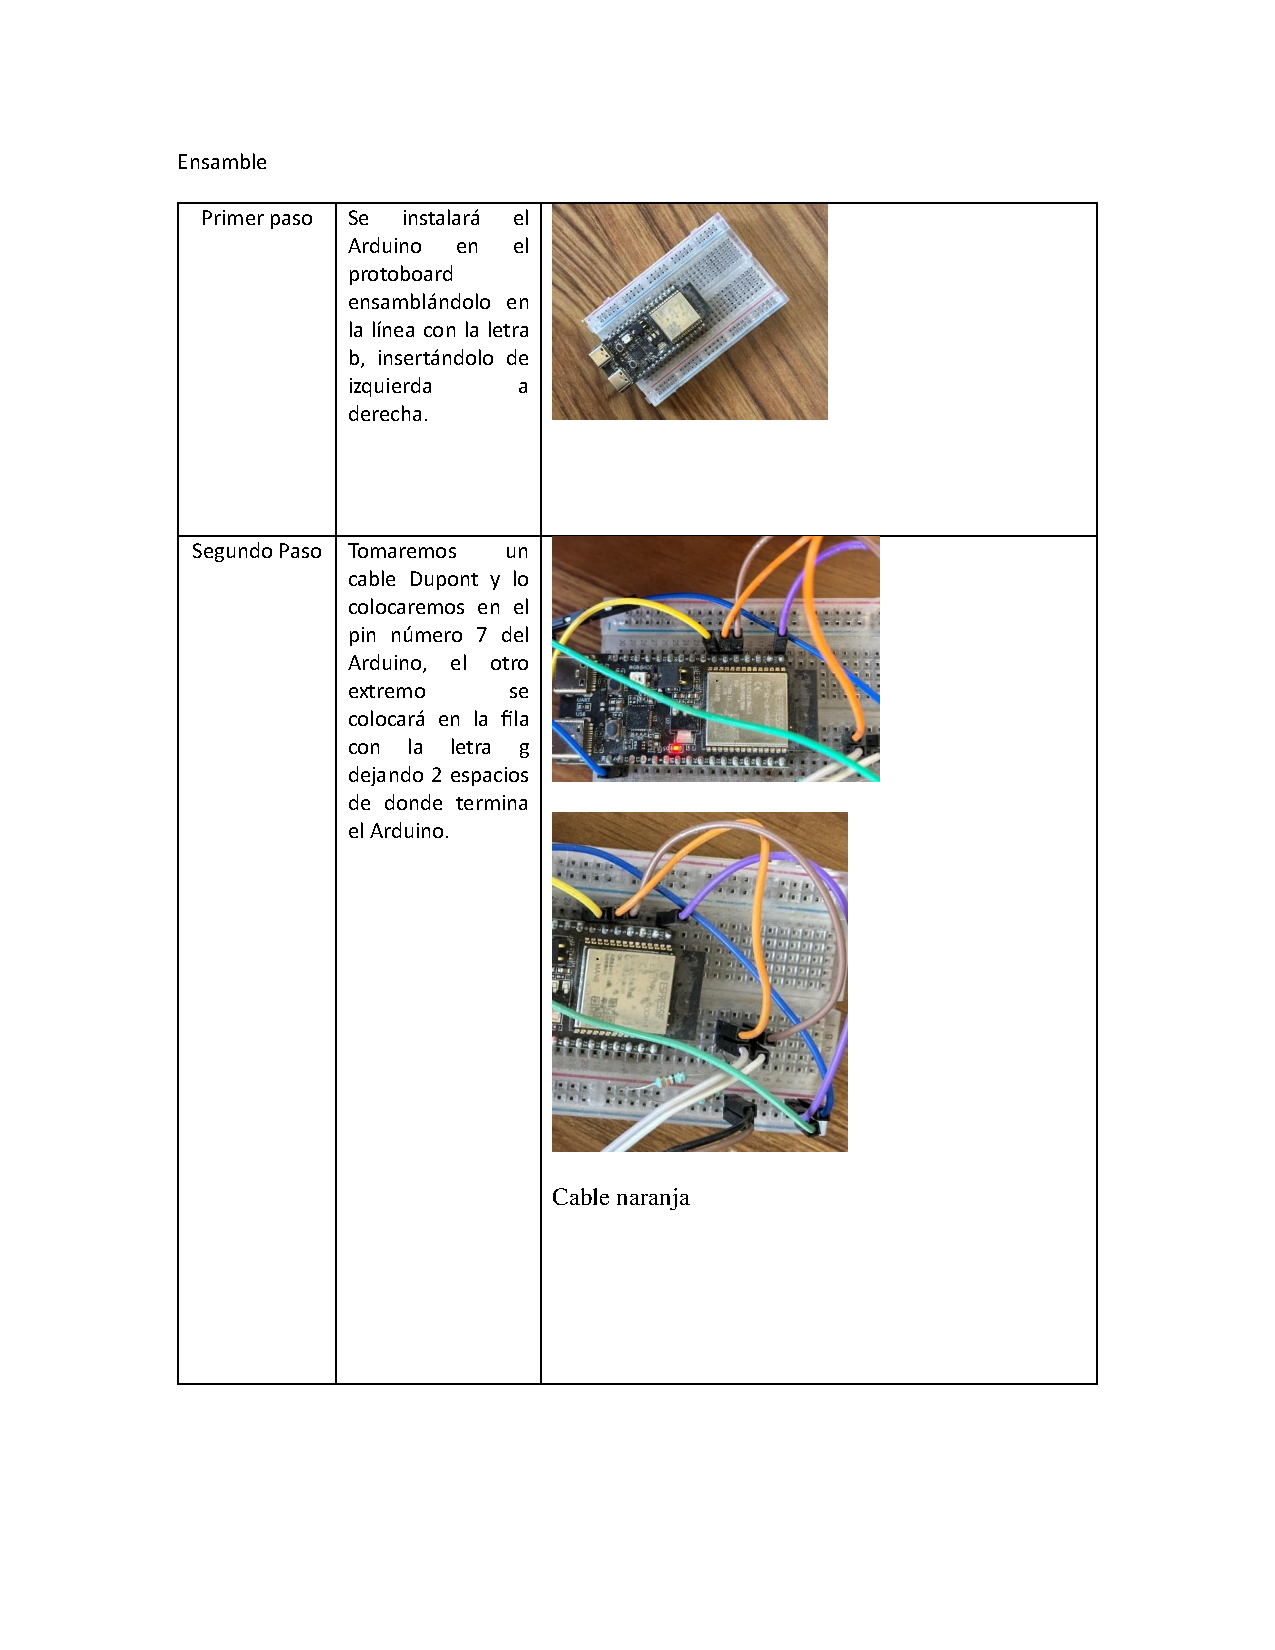
\includepdf[pages=-]{8/Img/Ensamble.pdf}
    \label{Ensamble}
    %%%%%%%%%%%%%%%%%%%%%%%%%%%%%%%%%%%%%%%%
    % 
    % 
    \centering{\section[\appendixautorefname{}]{APÉNDICE}}
    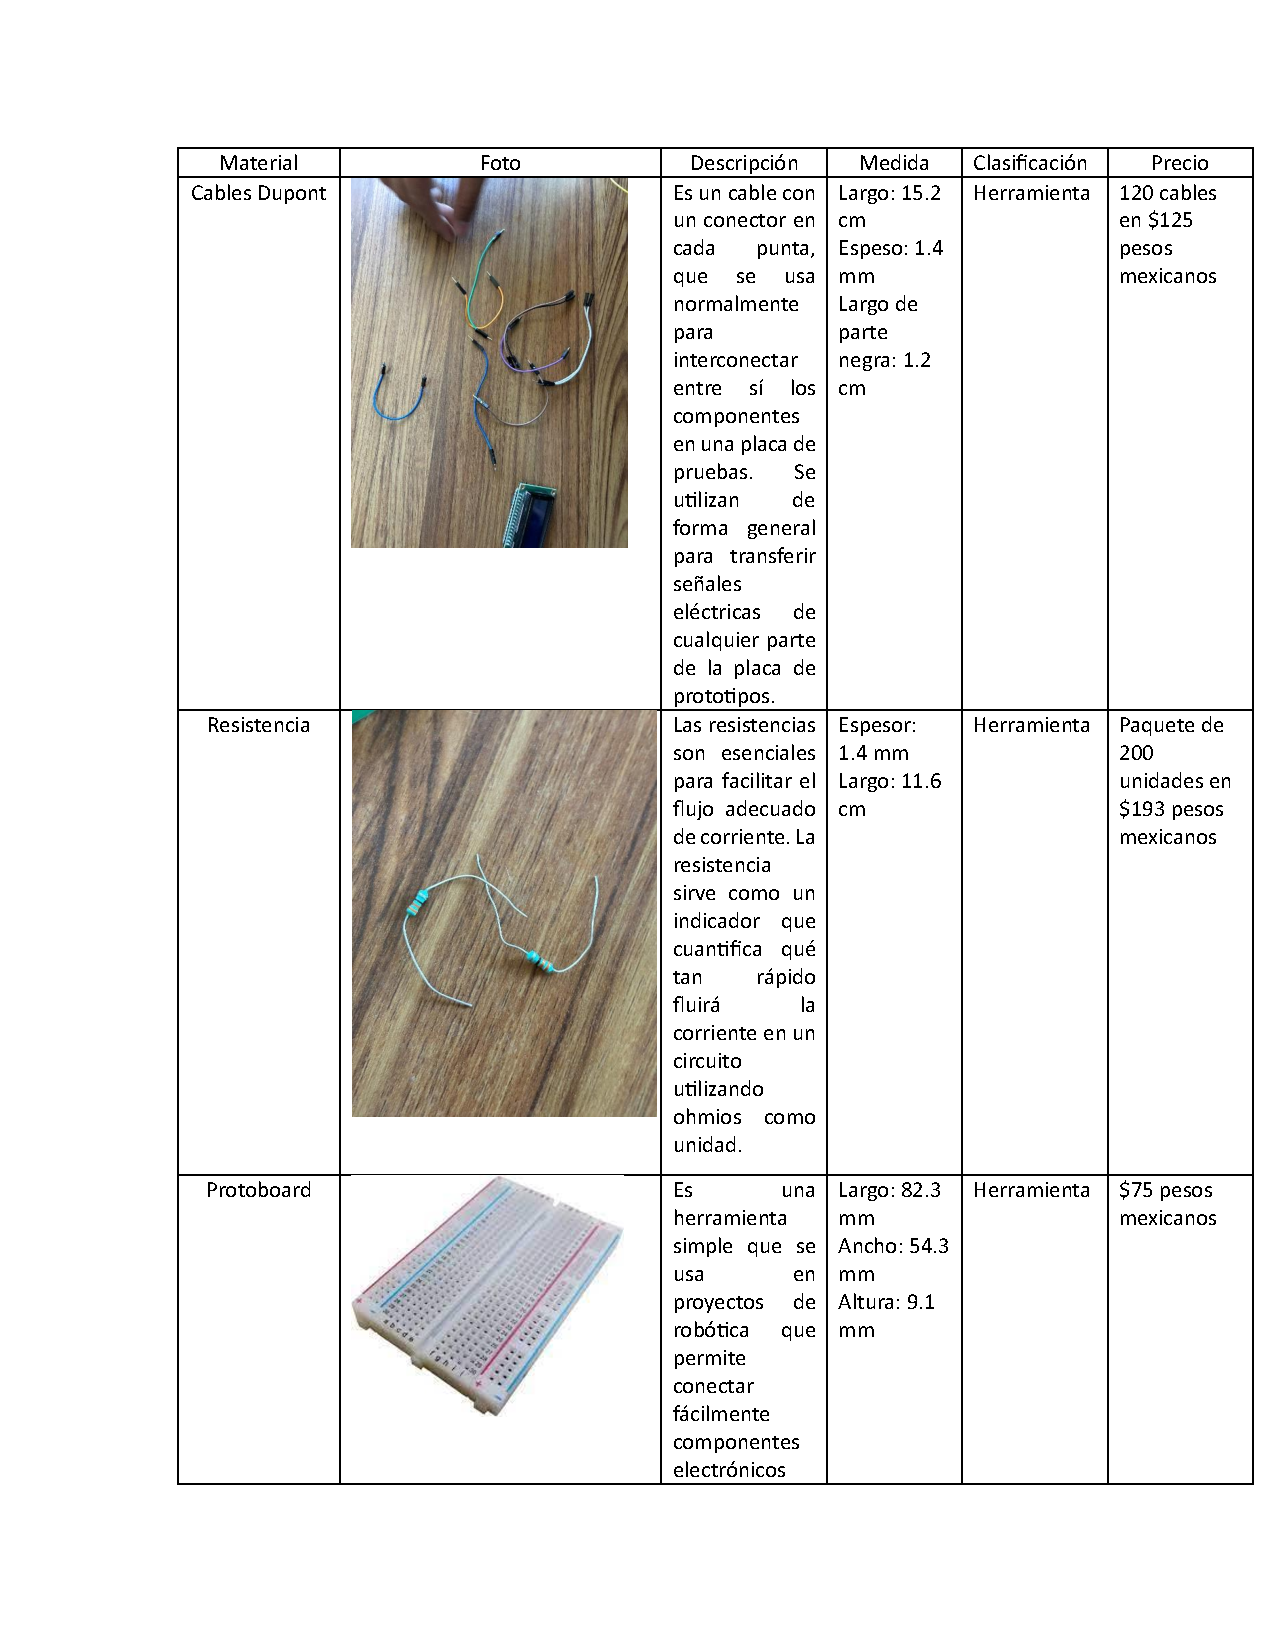
\includepdf[pages=-]{8/Img/Material.pdf}
    \label{Material}
    %%%%%%%%%%%%%%%%%%%%%%%%%%%%%%%%%%%%%%%%
    % 
    % 
    \centering{\section[\appendixautorefname{}]{APÉNDICE}}
    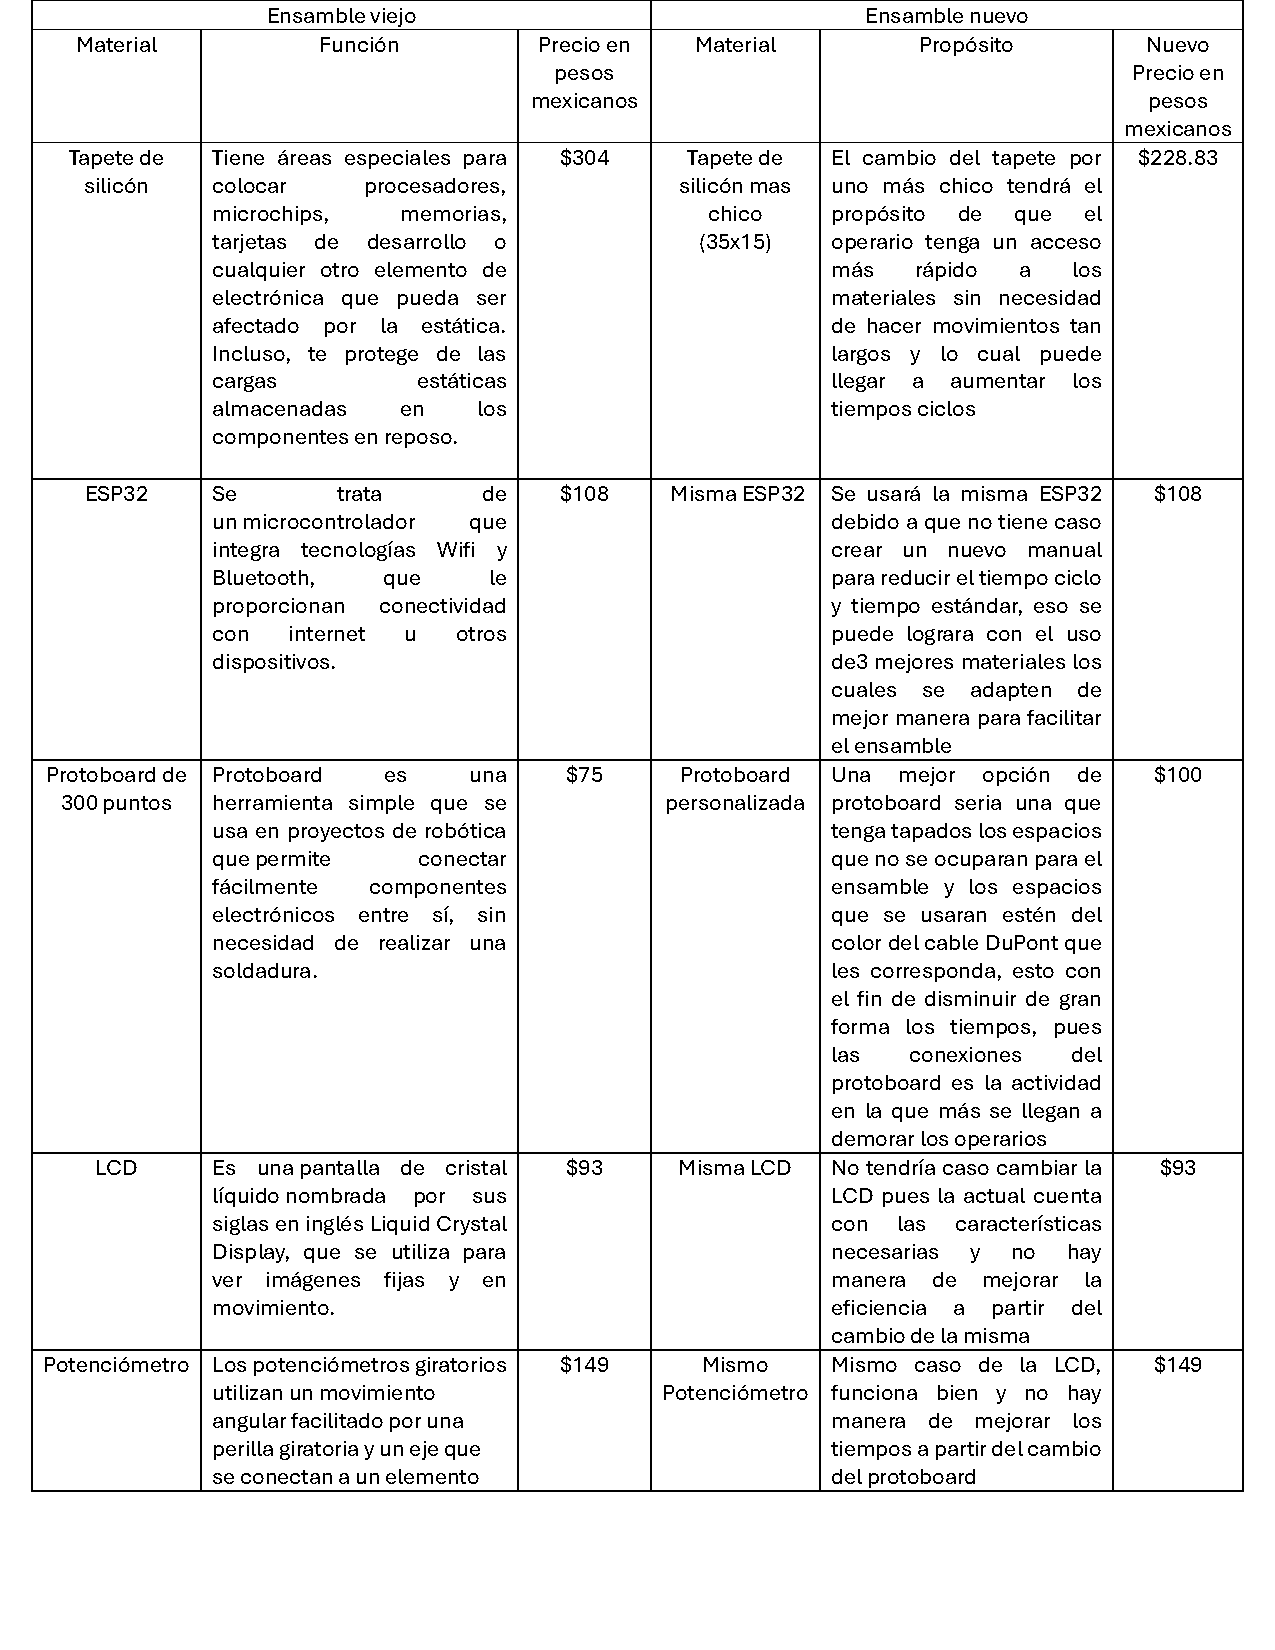
\includepdf[pages=-]{8/Img/Diseño de la forma más económica de realizar el trabajo}
    \label{Diseño para hacer mas economico el trabajo}
    %%%%%%%%%%%%%%%%%%%%%%%%%%%%%%%%%%%%%%%%
    % 
    % 
    \centering{\section[\appendixautorefname{}]{APÉNDICE}}
    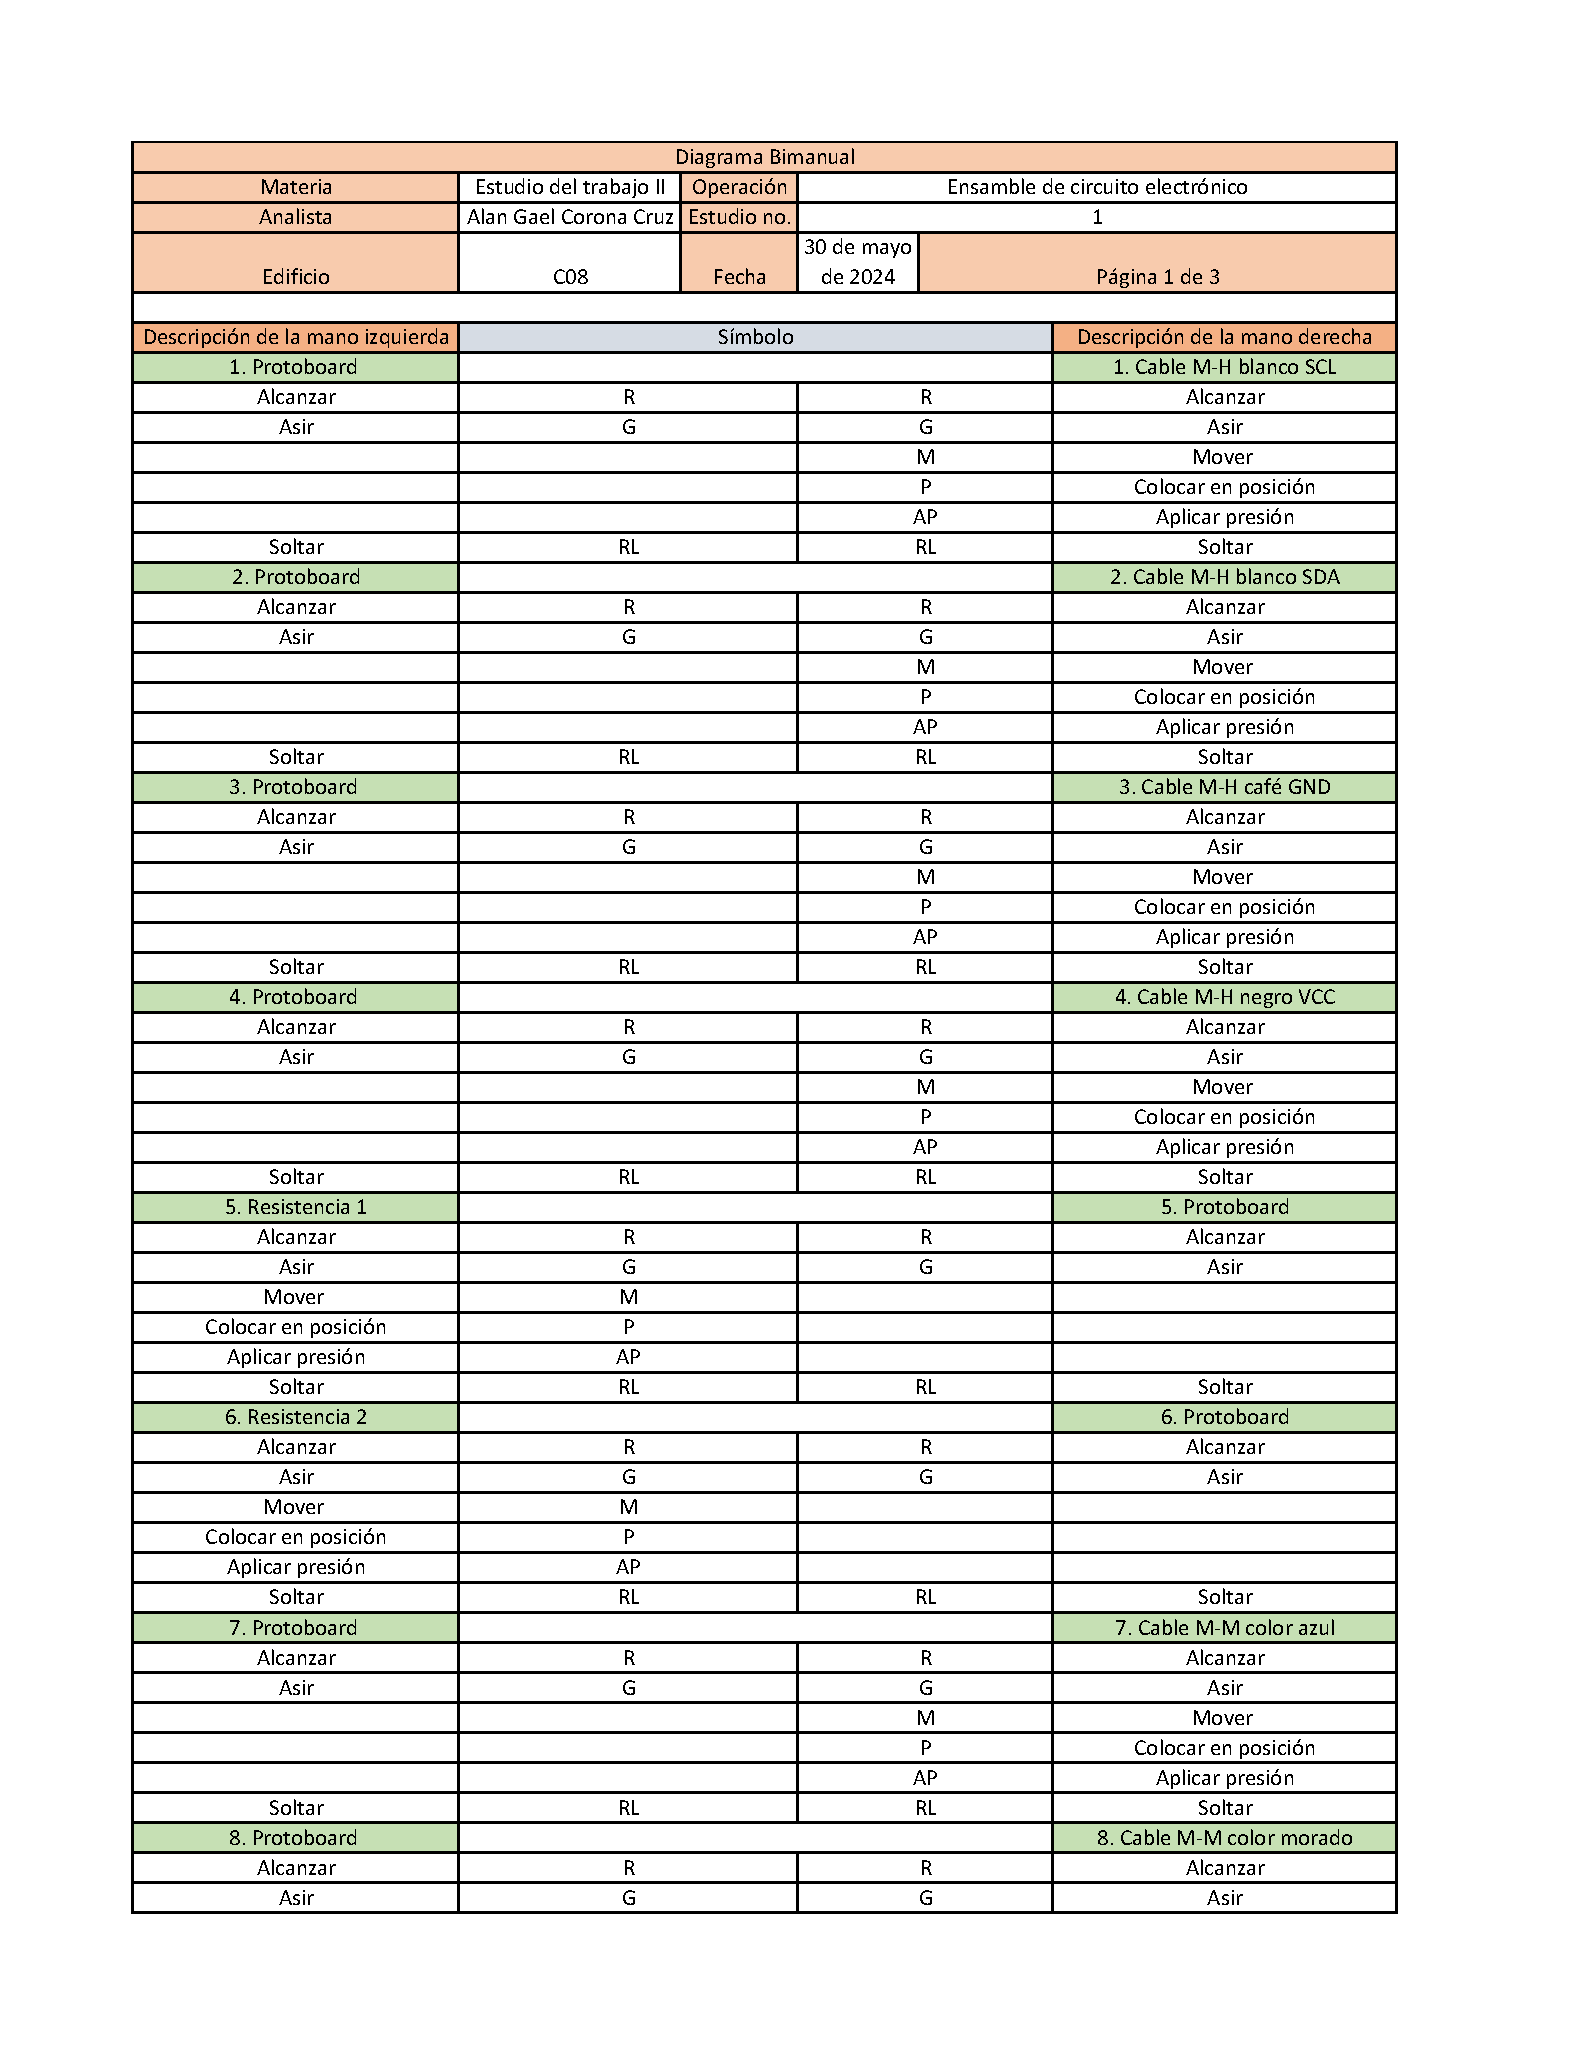
\includepdf[pages=-]{8/Img/diagramaBimanual}
    \label{Diagrama Bimanual}
    %%%%%%%%%%%%%%%%%%%%%%%%%%%%%%%%%%%%%%%%
    % 
    % 
    \centering{\section[\appendixautorefname{}]{APÉNDICE}}
    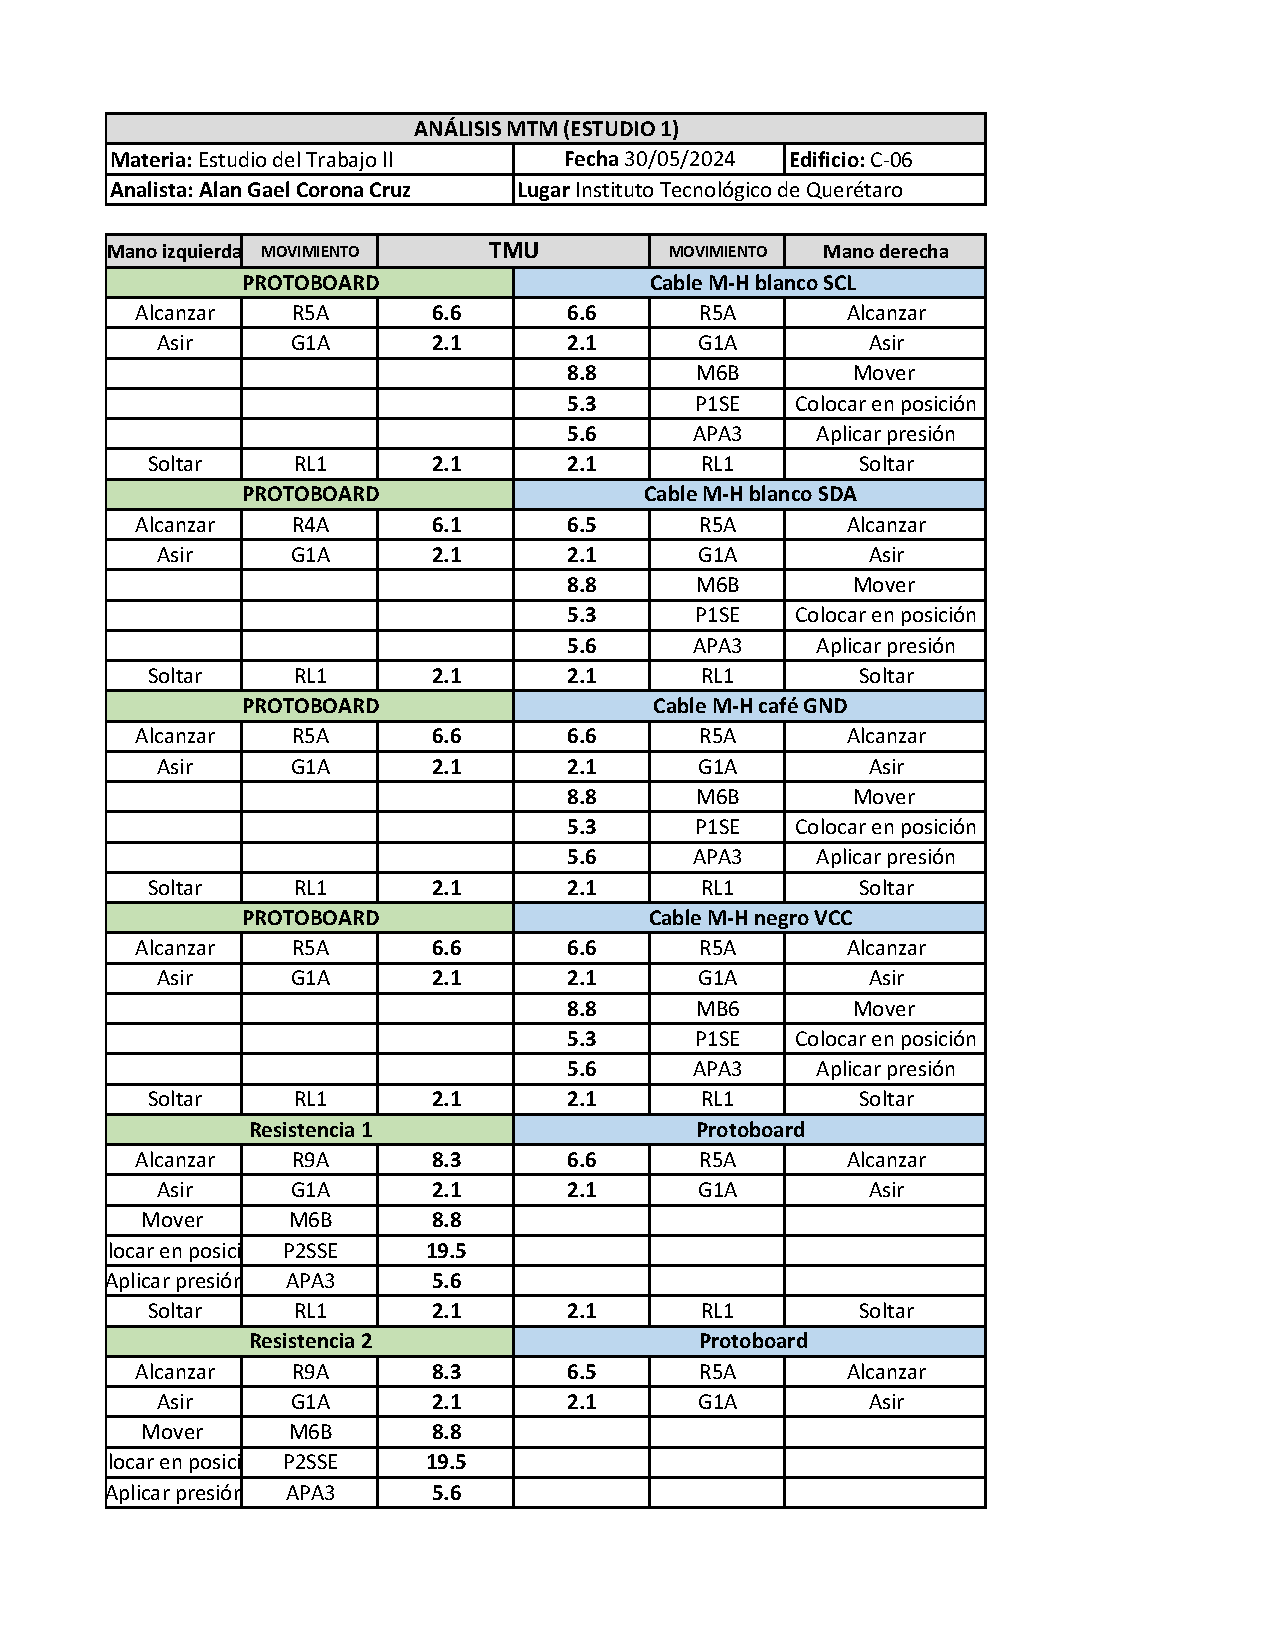
\includepdf[pages=-]{8/Img/UnidadesTmu}
    \label{Tabla de unidades TMU}
    %%%%%%%%%%%%%%%%%%%%%%%%%%%%%%%%%%%%%%%%
    \newpage
    \bibliographystyle{ieeetr}
    \bibliography{8/referencias}